\documentclass{tietreport}

% Essential packages
\usepackage{graphicx}
\usepackage{float}
\usepackage{amsmath}
\usepackage{amssymb}
\usepackage{booktabs}
\usepackage{tabularx}
\usepackage[hidelinks]{hyperref}
\hypersetup{
    hidelinks,
    colorlinks=false,
    pdfborder={0 0 0},
    linkbordercolor={1 1 1},
    citebordercolor={1 1 1},
    urlbordercolor={1 1 1},
    filebordercolor={1 1 1},
    menubordercolor={1 1 1},
    runbordercolor={1 1 1}
}
\usepackage{listings}
\usepackage{xcolor}

\definecolor{codegreen}{rgb}{0,0.6,0}
\definecolor{codegray}{rgb}{0.5,0.5,0.5}
\definecolor{codepurple}{rgb}{0.58,0,0.82}
\definecolor{backcolour}{rgb}{0.97,0.98,0.99}
\definecolor{codeblue}{rgb}{0.13,0.29,0.53}

\lstdefinestyle{pystyle}{
    backgroundcolor=\color{backcolour},   
    commentstyle=\color{codegreen}\itshape,
    keywordstyle=\color{codeblue}\bfseries,
    numberstyle=\tiny\color{codegray},
    stringstyle=\color{codepurple},
    basicstyle=\ttfamily\footnotesize,
    breakatwhitespace=false,         
    breaklines=true,                 
    captionpos=b,                    
    keepspaces=true,                 
    numbers=left,                    
    numbersep=6pt,                  
    showspaces=false,                
    showstringspaces=false,
    showtabs=false,                  
    tabsize=2,
    frame=single,
    rulecolor=\color{black!20},
    xleftmargin=12pt,
    framexleftmargin=10pt,
    aboveskip=8pt,
    belowskip=6pt,
    language=Python
}
\lstset{style=pystyle}

\setlength{\headheight}{15pt}

% Bibliography configuration
\usepackage[
  date=year,
  style=alphabetic,
  backend=bibtex,
  sorting=nty,
  maxnames=5,
  minnames=3,
  maxalphanames=4,
  minalphanames=3,
  backref=true,
  doi=false,
  isbn=false,
  url=false,
  eprint=false
]{biblatex}
\addbibresource{references.bib}

%% ==================================================
%% CUSTOMIZE THESE FIELDS FOR YOUR PROJECT
%% ==================================================

% Course/Lab header
\TitlePageHeader{%
  UCS503P - Software Engineering Project%
}

% Main project title
\ProjectTitle{%
  Cardio AI: Explainable Heart Disease Prediction%
}

% Subtitle or project description
\ProjectSubTitle{%
  Using CNN-LSTM Attention Network with Grad-CAM Interpretability%
}

% Student information (up to 4 students)
\author{%
  \texttt{1024170434} Dhruv Singla \\
  \texttt{1024170451} Srishti%
}

% Group number, degree, year, program
\TitlePageSubText{%
  Group: BE Third Year, CSE%
}

% Faculty advisor/guide name
\AdvisorName{%
  Dr. Nisha Thakur%
}

% Evaluation period and department info
\TitlePageFooterText{{%
    \large End Semester Evaluation \\[0.2cm]
    \bfseries Computer Science and Engineering Department%
  } \\[0.15cm]
  Thapar Institute of Engineering and Technology, Patiala%
}

%% ==================================================

\begin{document}

% Generate title page
\maketitle

% Table of contents (auto-generated from chapters)
\tableofcontents

% =========================================================================
% ===== CHAPTER 1: INTRODUCTION =====
% =========================================================================

\chapter{Introduction}
\label{chap:intro}

\section{Background and Context}

Cardiovascular disease remains the leading cause of mortality globally, accounting for an estimated 17.9 million deaths each year. This staggering clinical burden necessitates advanced, automated, non-invasive early-prediction systems. While deep learning models can predict heart disease from routine clinical measurements---such as blood pressure, cholesterol levels, resting ECG parameters, and exercise stress test metrics---their inherent ``black box'' nature poses a significant barrier to clinical adoption. Regulatory bodies (including the FDA and European medical regulatory frameworks) and medical ethics demand interpretable, auditable, and defensible predictions. 

This project, \textbf{Cardio AI}, aims to bridge this critical gap by prioritizing clinical transparency. Our objective is to translate complex deep neural network confidence scores into actionable, human-readable clinical narratives, empowering physicians to understand, verify, and trust AI-assisted diagnoses.

\subsection{Problem Statement}

While standard classification tasks can achieve high accuracy on clinical datasets, the primary challenge addressed by this project is shifting the focus from simple heart disease classification to \textbf{clinical transparency}---making deep learning explainable rather than an opaque black box. Current challenges in AI-driven heart disease prediction include:
\begin{itemize}
    \item \textbf{Black-Box Predictions:} Deep learning models, while highly accurate, offer no clinical reasoning or transparent decision pathways, leading to physician reluctance.
    \item \textbf{Feature Opacity:} The cardiovascular domain involves heterogeneous clinical features (e.g., numerical vitals, categorical ECG types, binary indicators). Understanding which specific physiological parameters drive a patient's risk score is non-trivial.
    \item \textbf{Operational Constraints \& Overfitting Risks:} Many theoretical models fail in practice due to overfitting on limited datasets (such as the UCI Cleveland dataset). Robust systems must deliver immediate value and incorporate strategies to fail fast through rapid iteration.
    \item \textbf{Lack of Visual Evidence:} Clinicians lack interactive visual artifacts (such as heatmaps or feature importance charts) that map model confidence directly back to patient physiology.
    \item \textbf{Absence of Longitudinal Tracking:} Existing diagnostic tools rarely support patient-history-aware predictions or longitudinal trend analysis across repeated assessments.
\end{itemize}

\section{Project Objectives}

To address these challenges, we have defined the following core SMART (Specific, Measurable, Achievable, Relevant, Time-bound) objectives:
\begin{enumerate}
    \item \textbf{Develop an Explainable Deep Learning Model:} Architect and train a hybrid CNN-LSTM-Attention model on the UCI Cleveland Heart Disease dataset. This model incorporates multiple Explainable AI (XAI) methods, specifically Grad-CAM, Attention weights, and SHAP (Shapley Additive exPlanations), to decode the model's internal reasoning.
    \item \textbf{Deliver an Interactive Clinical Dashboard:} Create a responsive, premium Single Page Application (SPA) using HTML5, CSS3, Bootstrap 5, and JavaScript. This dashboard allows clinicians to input physiological parameters and visualize predictions via Plotly.js interactive charts.
    \item \textbf{Automate Clinical Reporting:} Generate automated PDF reports featuring AI-driven narrative summaries, feature-by-feature clinical interpretations, and guideline-referenced evaluations.
    \item \textbf{Implement Patient Management Architecture:} Design a robust backend using Flask (Python) and a relational database (MySQL) to securely track longitudinal patient records and audit histories.
    \item \textbf{Rigorous Software Quality and Test Validation:} Execute comprehensive unit, integration, and end-to-end software test suites validating system functionality, boundary integrity, and XAI concordance.
\end{enumerate}


% =========================================================================
% ===== CHAPTER 2: METHODOLOGY & DESIGN =====
% =========================================================================

\chapter{Methodology and Design}
\label{chap:methodology}

\section{System Architecture and Design Methodology}
\label{sec:system_methodology}

To address the clinical opacity of black-box machine learning in cardiovascular care, Cardio AI is designed around a multi-tier, service-oriented architecture. The system unites deep spatiotemporal feature representation with multi-method explainability consensus and evidence-based clinical guideline decision support.

\subsection{Design Methodology and Core Objectives}

The engineering methodology focuses on four core principles:
\begin{itemize}
    \setlength{\itemsep}{1pt}\setlength{\parskip}{0pt}
    \item \textbf{Spatiotemporal Feature Representation:} Converting 1D tabular patient vitals into 2D polar image representations via Gramian Angular Summation Fields (GASF), preserving non-linear pairwise interactions without artificial spatial assumptions.
    \item \textbf{Hybrid Neural Modeling:} Combining 2D Convolutional Neural Networks (CNN) for spatial biomarker pattern extraction with Bidirectional LSTM for sequential dependencies and Hierarchical Self-Attention for diagnostic weighting.
    \item \textbf{Multi-Method Explainability Consensus:} Eliminating single-algorithm bias by computing Grad-CAM, Kernel SHAP, and Self-Attention concurrently, validating alignment via Spearman rank correlation and top-4 Jaccard feature overlap.
    \item \textbf{Evidence-Based Clinical Guidance:} Coupling predictions with ACC/AHA 2017 clinical guidelines to synthesize automated natural language patient narratives and structured cardiology recommendations.
\end{itemize}

\subsection{Clinical Telemetry and Preprocessing Methodology}

The data foundation utilizes the benchmark UCI Cleveland Heart Disease dataset (303 patient records across 13 physiological parameters):
\begin{itemize}
    \setlength{\itemsep}{1pt}\setlength{\parskip}{0pt}
    \item \textbf{Demographics and Hemodynamics:} Age (29--77 years), biological sex, resting systolic blood pressure (94--200 mmHg), and serum cholesterol (126--564 mg/dL).
    \item \textbf{Metabolic, Electrical, and Stress Vitals:} Fasting blood sugar ($>120$ mg/dL), resting ECG status, maximum exercise heart rate (71--202 bpm), exercise angina, ST depression (0.0--6.2 mm), and peak ST slope.
    \item \textbf{Invasive Imaging Biomarkers:} Major vessels colored by fluoroscopy (0--3) and thallium scintigraphy defect status (normal, fixed, or reversible defect).
\end{itemize}

The preprocessing pipeline implements four robust safeguards:
\begin{itemize}
    \setlength{\itemsep}{1pt}\setlength{\parskip}{0pt}
    \item \textbf{Imputation:} Median imputation for continuous variables and mode imputation for categorical attributes to preserve sample size without bias.
    \item \textbf{Bounded Rescaling:} MinMax scaling of all numerical values to the range between -1 and 1 for stable polar trigonometric encoding.
    \item \textbf{Categorical Expansion:} One-hot encoding multi-class categorical features, expanding the clinical feature space from 13 raw vitals to 28 orthogonal representations.
    \item \textbf{Stratified Class Balancing:} Applying Synthetic Minority Over-sampling Technique (SMOTE) strictly to training partitions within 5-fold cross-validation, protecting test partitions from data leakage.
\end{itemize}

\subsection{Spatiotemporal 2D GASF Transformation Design}

Standard convolutional networks require 2D spatial structures. To apply 2D convolutions to 1D tabular records without assuming artificial feature ordering, normalized clinical features are mapped into polar coordinates. Pairwise trigonometric cosine summation generates a 28 by 28 Gramian Angular Summation Field tensor. The diagonal elements preserve individual feature amplitudes, while off-diagonal elements capture non-linear, cross-vital correlations across the entire patient profile.

\subsection{Hybrid Deep Learning Architecture Design}

The predictive neural engine is structured into four functional stages:
\begin{enumerate}
    \setlength{\itemsep}{1pt}\setlength{\parskip}{0pt}
    \item \textbf{Spatial Convolutional Branch (2D CNN):} Two sequential convolutional blocks (32 and 64 filters with 3 by 3 kernels, Batch Normalization, Spatial Dropout of 0.20, and Max-Pooling) extract localized spatial patterns from the 28 by 28 GASF tensor.
    \item \textbf{Sequential Recurrent Branch (Bidirectional LSTM):} The resulting feature map is reshaped into an ordered sequence of 49 spatial tokens with 64 channels each. A Bidirectional LSTM layer (64 units per direction, 128 total) models sequential cross-feature transitions and progressive cardiovascular deterioration patterns.
    \item \textbf{Hierarchical Self-Attention Mechanism:} An additive self-attention layer scores the recurrent hidden states against a learned query vector, producing an attention-weighted context vector that dynamically highlights the most decisive diagnostic biomarkers.
    \item \textbf{Classification Head:} A fully connected layer with L2 regularization, dropout of 0.30, and a Sigmoid activation unit outputs a calibrated posterior probability of heart disease presence. The network is trained using Binary Cross-Entropy loss and the Adam optimizer with early stopping and learning rate scheduling.
\end{enumerate}

\subsection{Multi-Method Explainable AI (XAI) Consensus Design}

To ensure clinical interpretability and satisfy medical validation standards, Cardio AI combines three distinct explanation paradigms:
\begin{itemize}
    \setlength{\itemsep}{1pt}\setlength{\parskip}{0pt}
    \item \textbf{2D Grad-CAM:} Computes gradients of the predicted risk class with respect to the final convolutional feature maps, highlighting localized spatial feature intersections that drive risk.
    \item \textbf{Kernel SHAP:} Calculates additive Shapley values based on cooperative game theory, determining the positive or negative contribution of each clinical feature relative to the population baseline.
    \item \textbf{Intrinsic Self-Attention:} Directly extracts normalized attention weights from the neural network forward pass without post-hoc surrogate approximations.
\end{itemize}
The system validates explanation concordance using Spearman rank correlation and the Jaccard similarity index across the top-4 features. When both metrics meet target thresholds (Spearman correlation of at least 0.60 and Jaccard overlap of at least 0.50), the prediction receives a High Clinician Confidence verification badge.

\subsection{Evidence-Based Clinical Decision Support Design}

To ground predictive scores in medical practice, the system incorporates an evidence-based clinical rule engine:
\begin{itemize}
    \setlength{\itemsep}{1pt}\setlength{\parskip}{0pt}
    \item \textbf{Decoupled Clinical Guidelines:} Declarative thresholds from the 2017 ACC/AHA guidelines (Stage 2 Hypertension at 140 mmHg or higher, Dyslipidemia at 240 mg/dL or higher, Myocardial Ischemia at ST depression 1.0 mm or higher, and Chronotropic Incompetence below 85 percent of max heart rate) are maintained in an external JSON schema.
    \item \textbf{Automated Narrative Synthesis:} The engine links patient vitals with top consensus XAI drivers, decomposing findings into primary risk drivers and secondary observations, and automatically generates natural language diagnostic summaries and cardiology referral recommendations.
\end{itemize}

\subsection{System Decomposition and Multi-Tier Architecture}

The Cardio AI platform is organized into four decoupled tiers:
\begin{enumerate}
    \setlength{\itemsep}{1pt}\setlength{\parskip}{0pt}
    \item \textbf{Presentation Tier:} A responsive Single Page Application built with HTML5, CSS3 glassmorphism, Bootstrap 5, Three.js and Vanta.js 3D backgrounds, Plotly.js interactive charts, and Web Audio API synthesized acoustic feedback.
    \item \textbf{Middleware Tier:} A Python Flask REST API managing payload validation, inference execution, consensus scoring, and automated ReportLab PDF report generation.
    \item \textbf{Inference Tier:} A high-performance machine learning runtime executing vectorized GASF projection, neural inference, and parallel XAI generation.
    \item \textbf{Persistence Tier:} A relational MySQL database maintaining patient demographics, historical clinical records, AI diagnoses, and audit logs.
\end{enumerate}


\clearpage
\clearpage
\section{System Modeling and Project Diagrams}
\label{sec:system_modeling}

To provide a comprehensive blueprint of the Cardio AI system, several architectural and behavioral models were developed across the 20-week engineering lifecycle.

\subsection{Project Scheduling and Timeline (Gantt Chart)}

Project implementation followed a structured 20-week schedule organized into five concurrent development tracks (Literature Review, Data Engineering, Neural Modeling, Explainability and Clinical Guidelines, and Web Integration). Figure~\ref{fig:gantt} illustrates the project timeline, major milestones, and assessment reviews.

\begin{figure}[H]
    \centering
    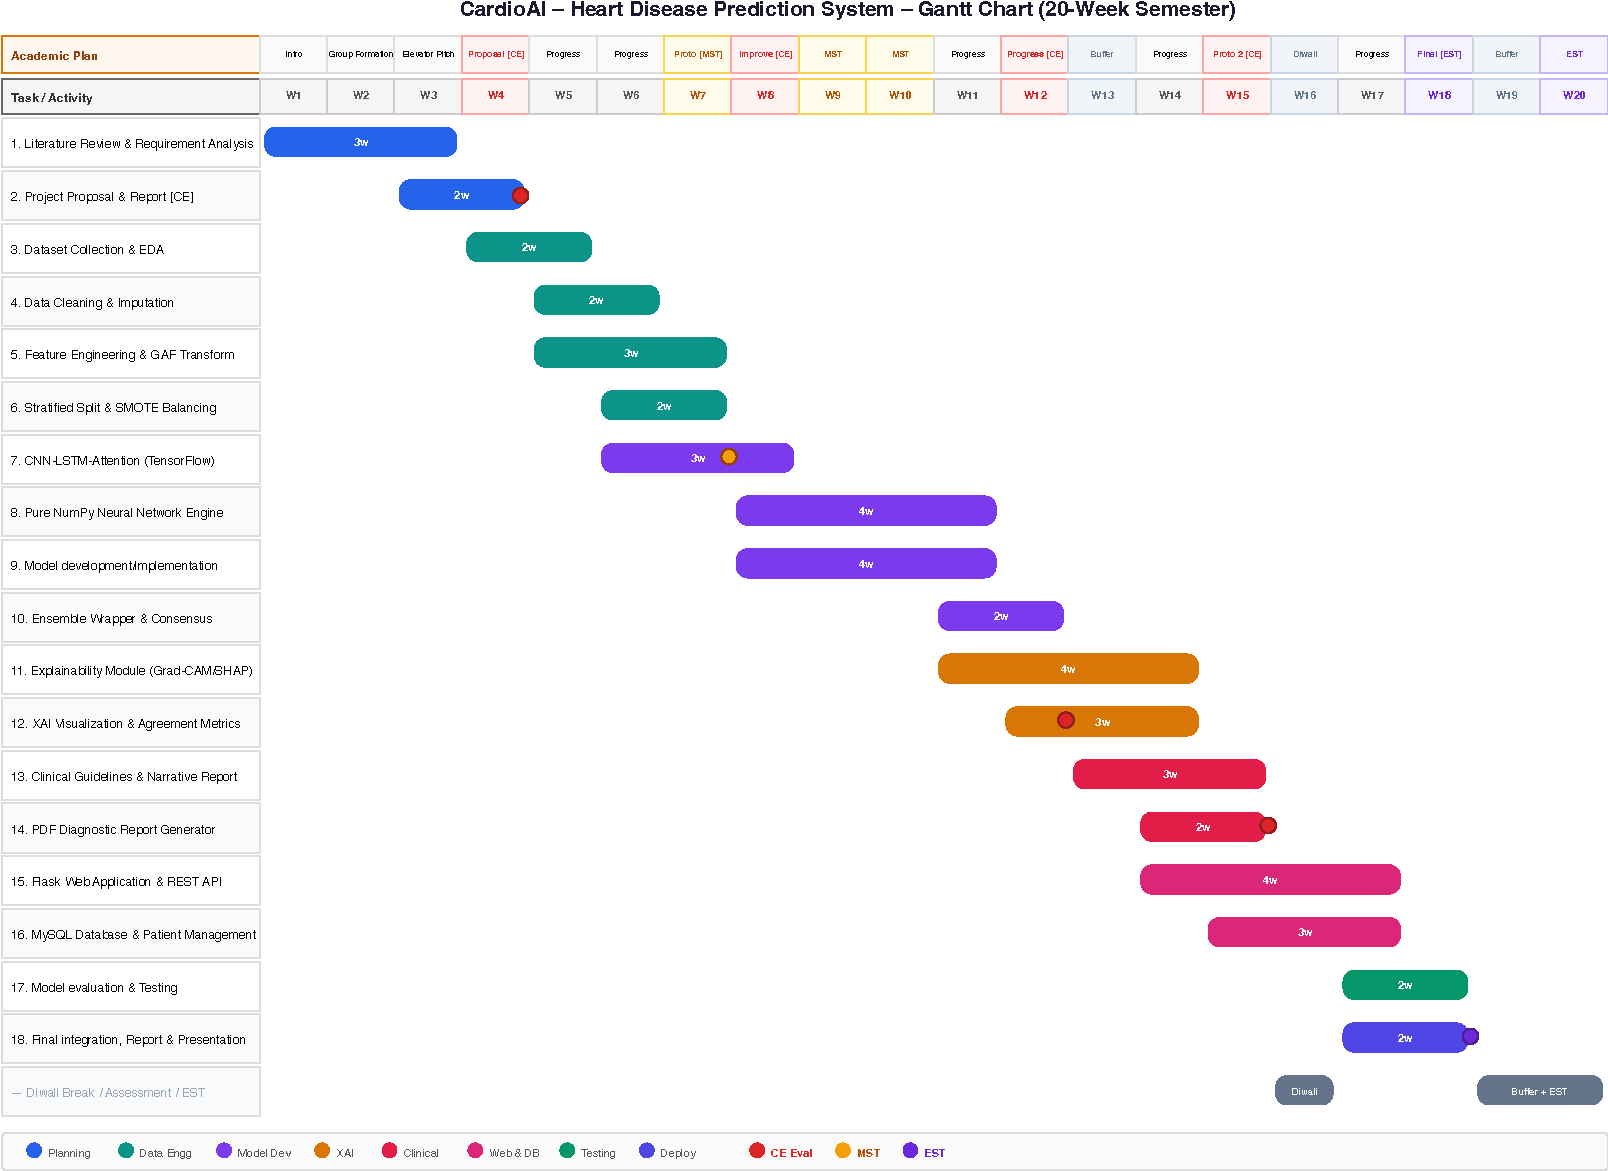
\includegraphics[width=\textwidth,height=0.62\textheight,keepaspectratio]{diagrams/ganttchart.pdf}
    \caption{Project Scheduling and Timeline (Gantt Chart)}
    \label{fig:gantt}
\end{figure}
\clearpage
\subsection{UML Use Case Diagram}
\begin{figure}[H]
    \centering
    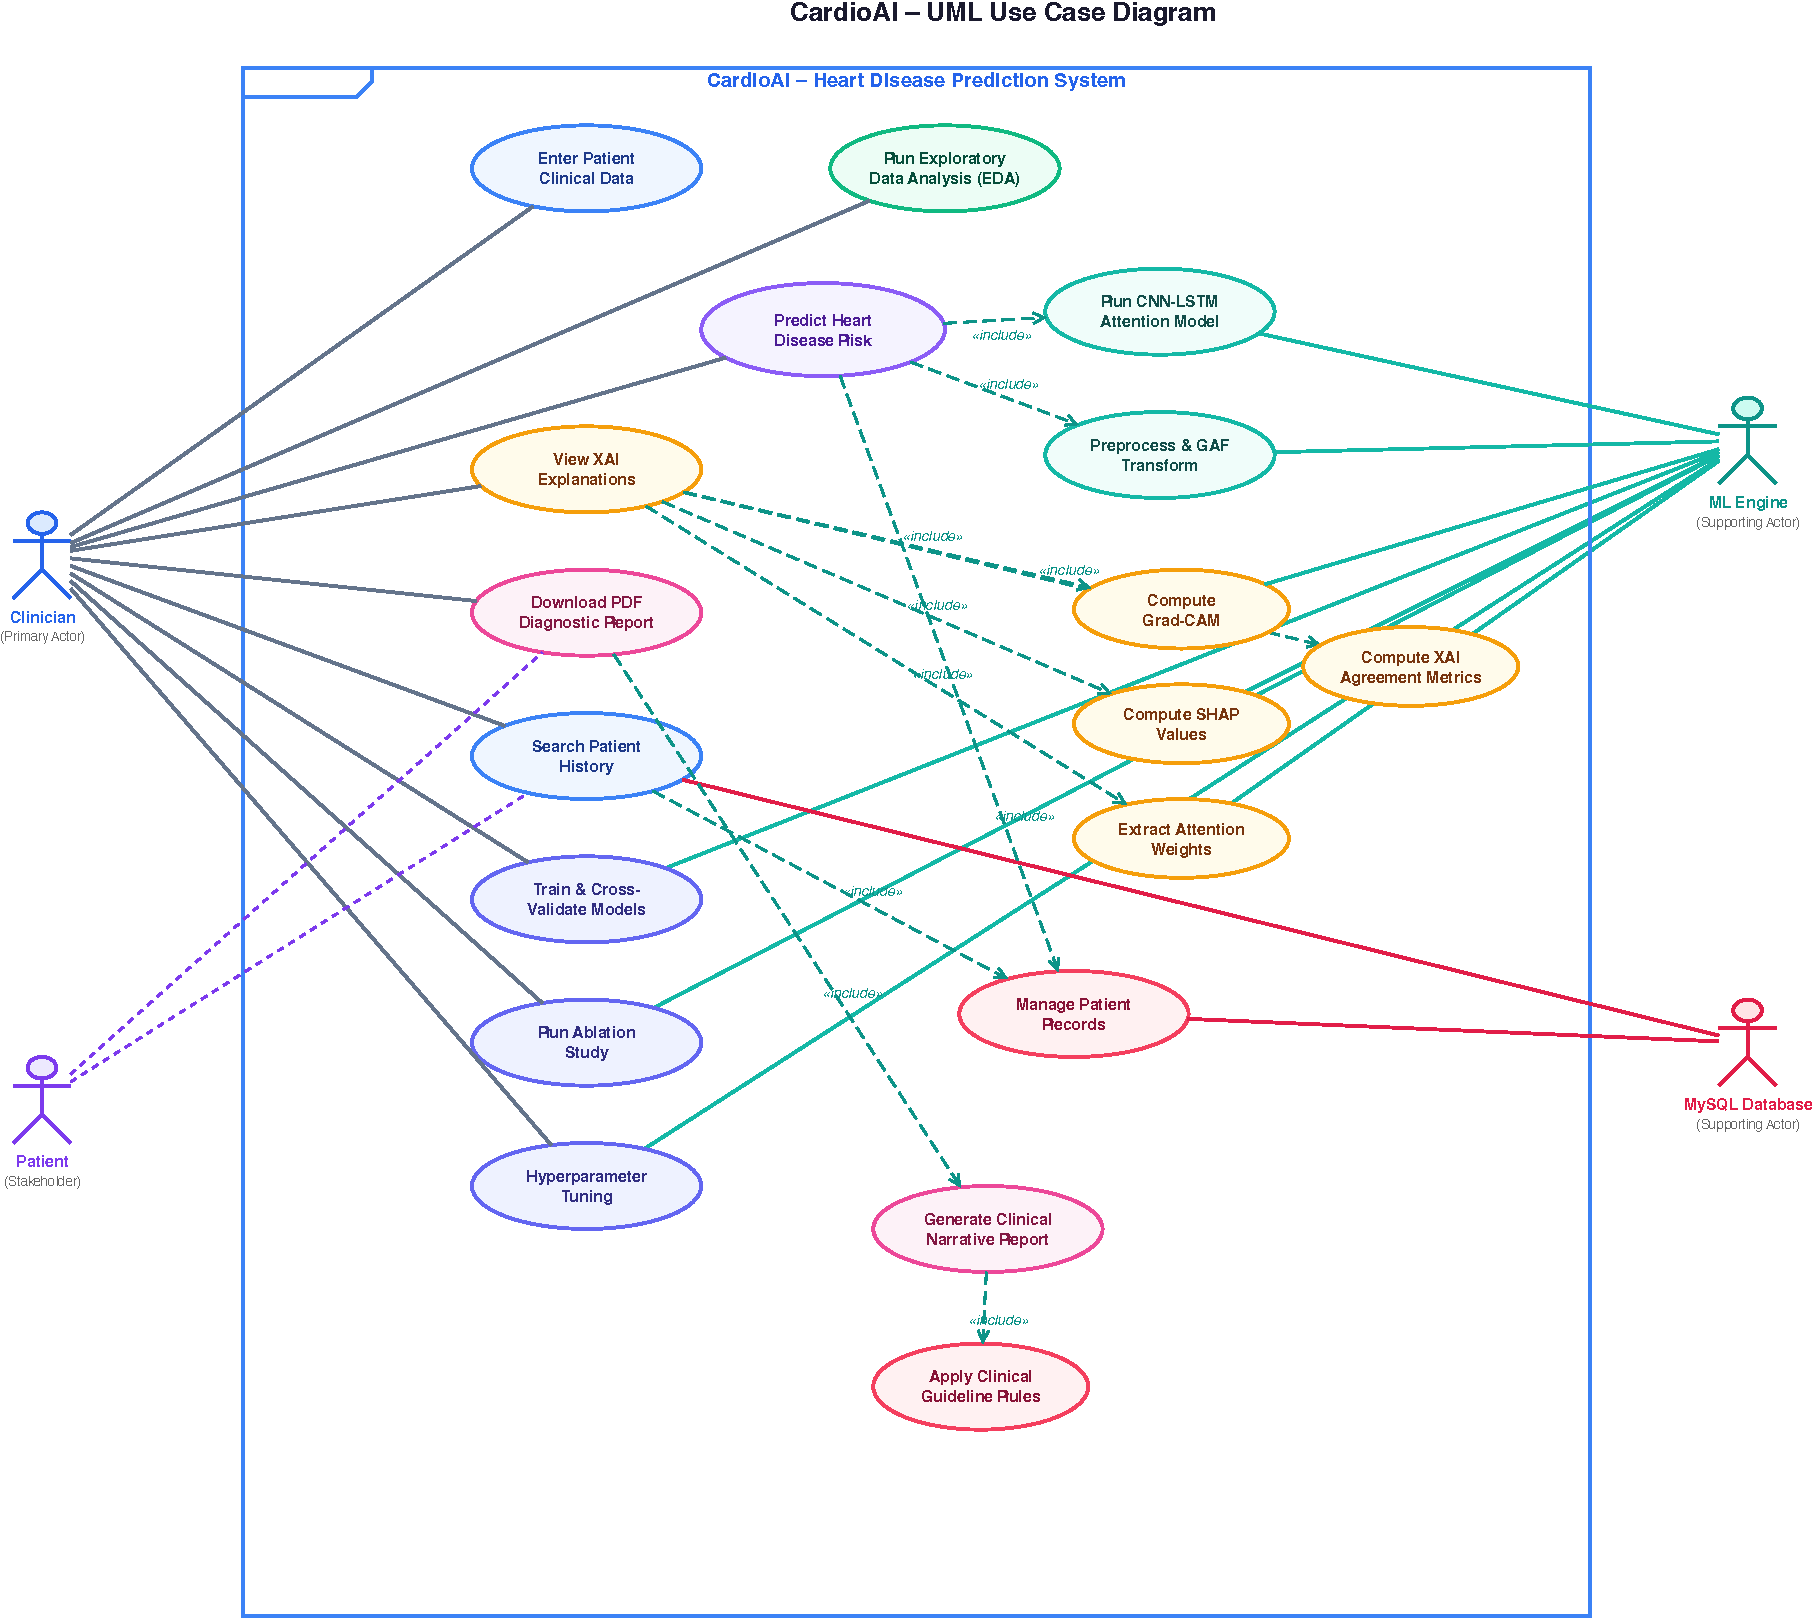
\includegraphics[width=\textwidth,height=0.82\textheight,keepaspectratio]{diagrams/use case diagram.pdf}
    \caption{UML Use Case Diagram identifying system boundaries and primary actors.}
    \label{fig:usecase}
\end{figure}

\subsection{Use Case Specifications}
The following sections detail the specific use case templates that define the interactions between actors and the Cardio AI system.

\begin{figure}[H]
    \centering
    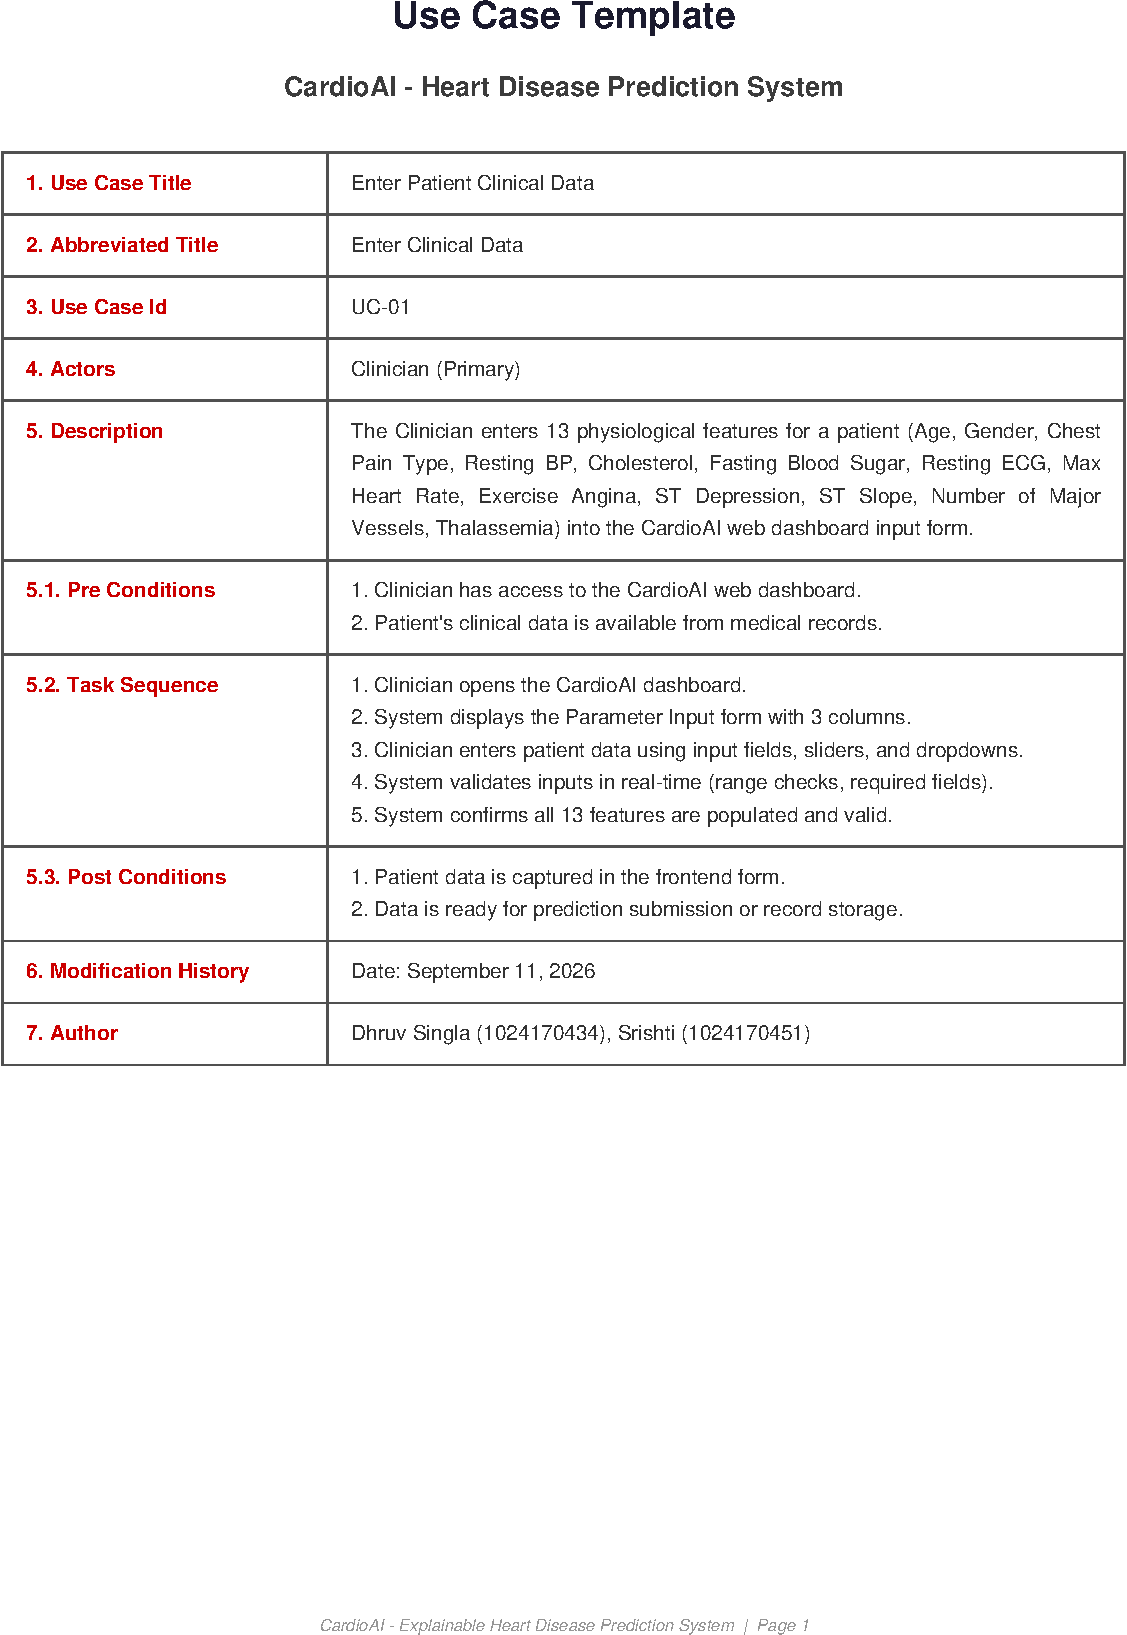
\includegraphics[width=\textwidth,height=0.82\textheight,keepaspectratio]{diagrams/use_case_templates/UC_01_Enter_Clinical_Data.pdf}
    \caption{Use Case: Enter Clinical Data}
\end{figure}
\clearpage

\begin{figure}[H]
    \centering
    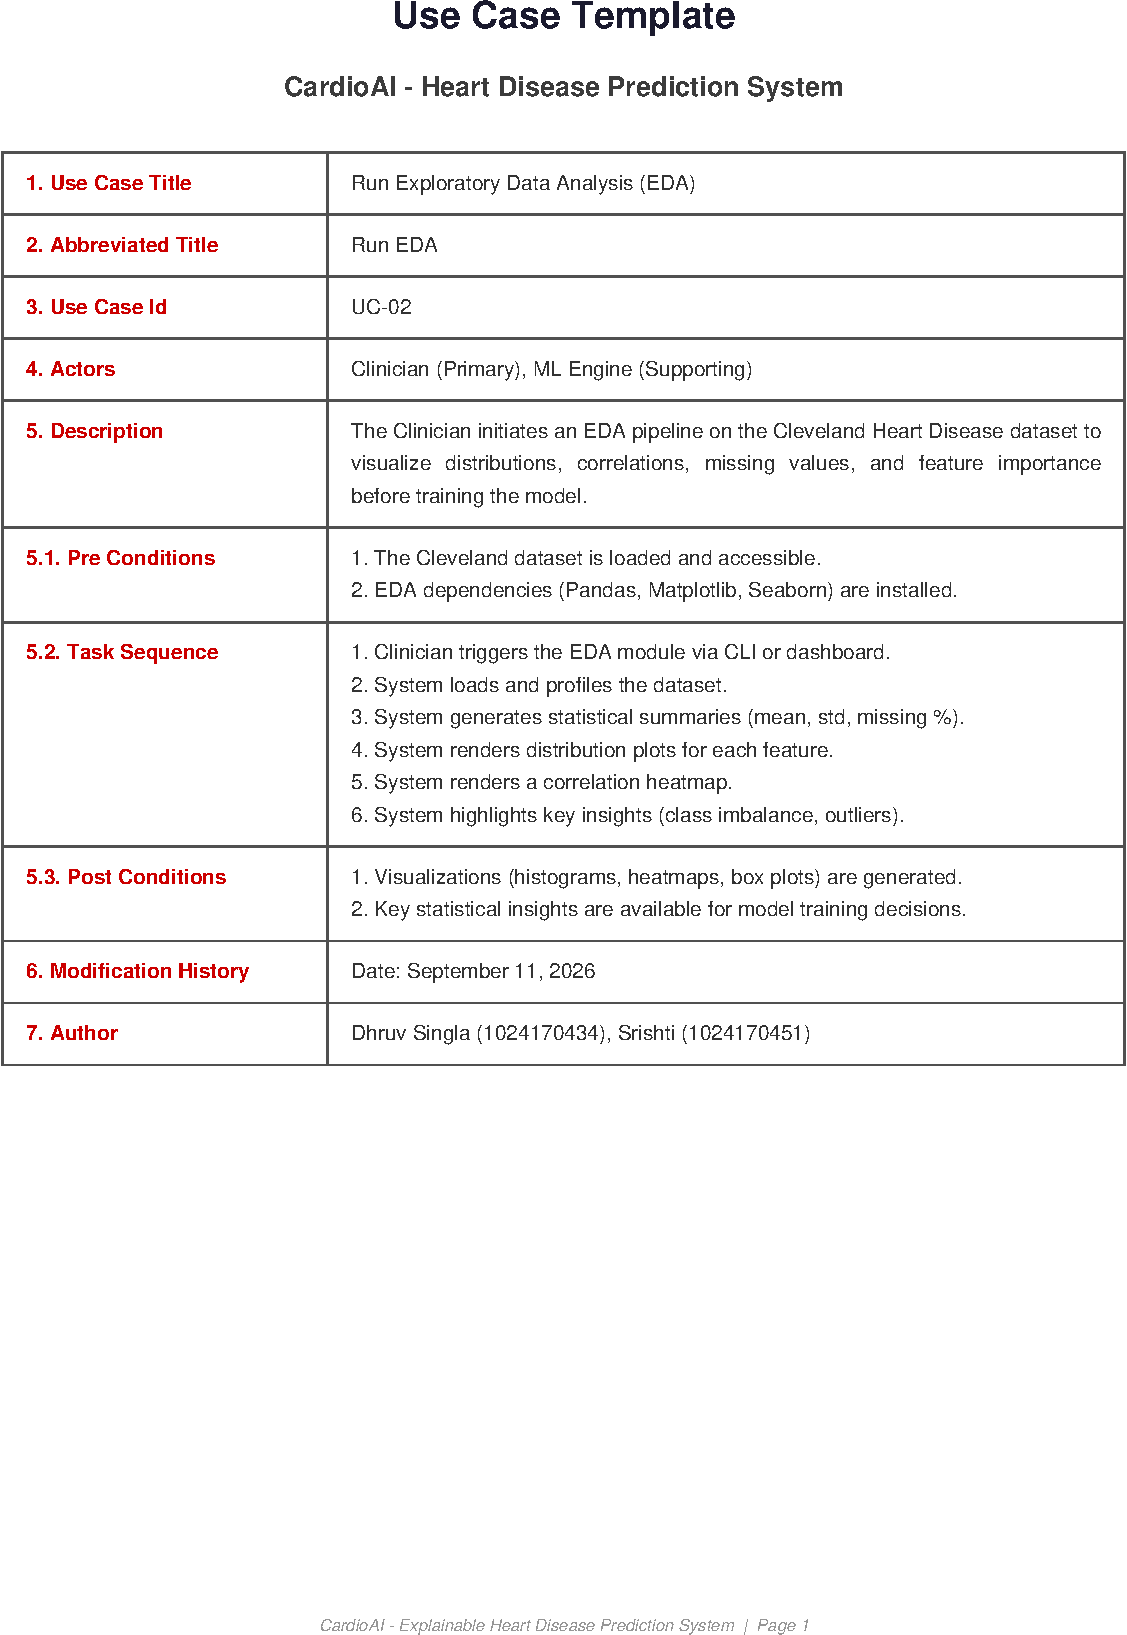
\includegraphics[width=\textwidth,height=0.82\textheight,keepaspectratio]{diagrams/use_case_templates/UC_02_Run_EDA.pdf}
    \caption{Use Case: Run EDA}
\end{figure}
\clearpage

\begin{figure}[H]
    \centering
    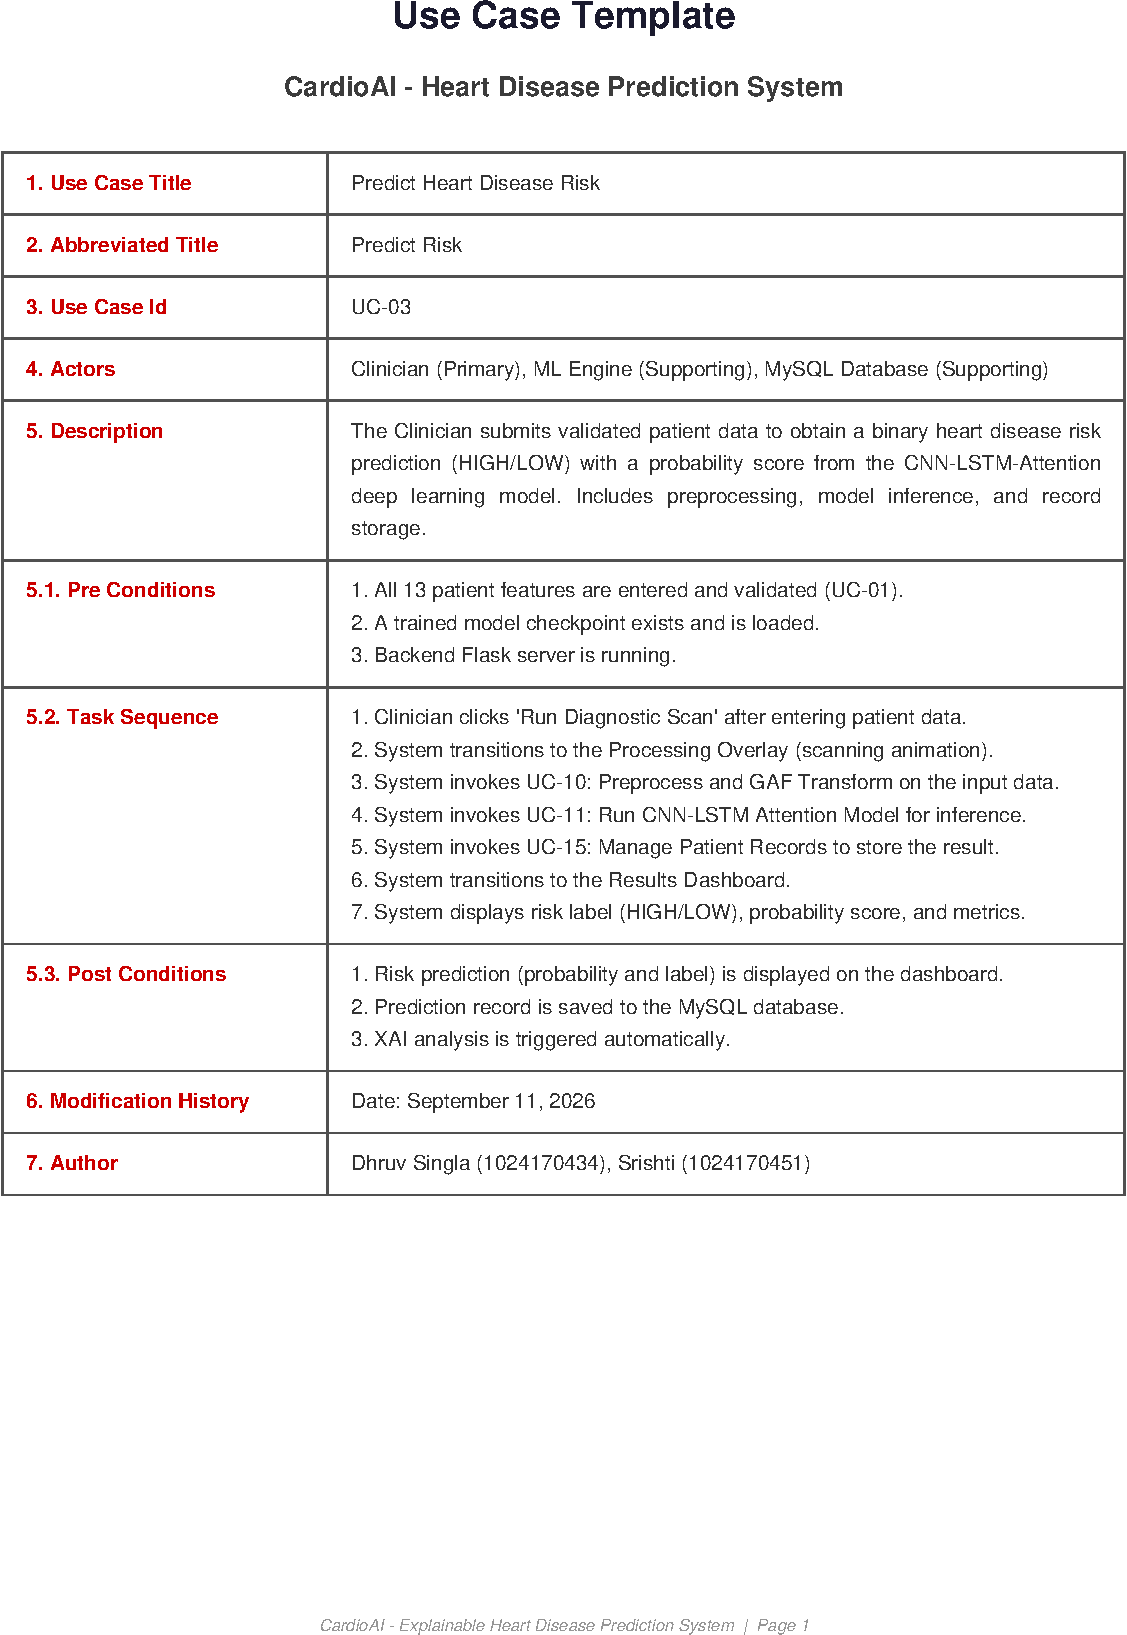
\includegraphics[width=\textwidth,height=0.82\textheight,keepaspectratio]{diagrams/use_case_templates/UC_03_Predict_Risk.pdf}
    \caption{Use Case: Predict Risk}
\end{figure}
\clearpage

\begin{figure}[H]
    \centering
    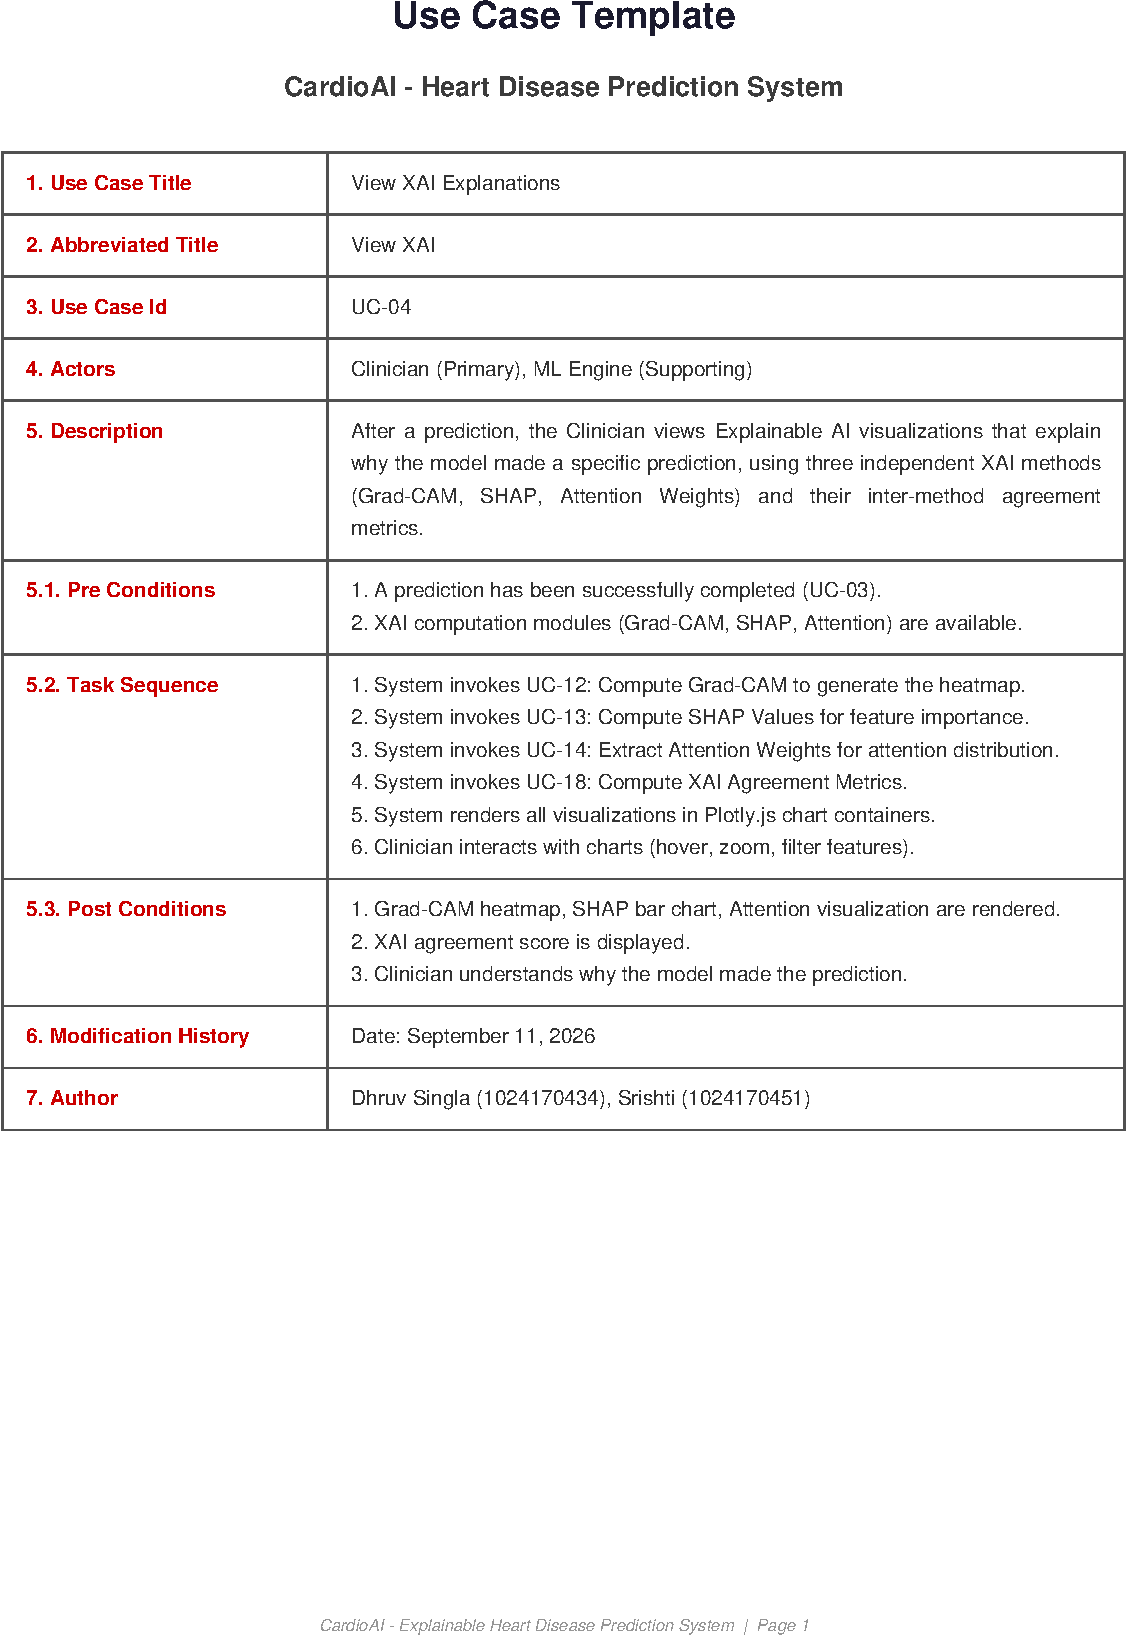
\includegraphics[width=\textwidth,height=0.82\textheight,keepaspectratio]{diagrams/use_case_templates/UC_04_View_XAI.pdf}
    \caption{Use Case: View XAI}
\end{figure}
\clearpage

\begin{figure}[H]
    \centering
    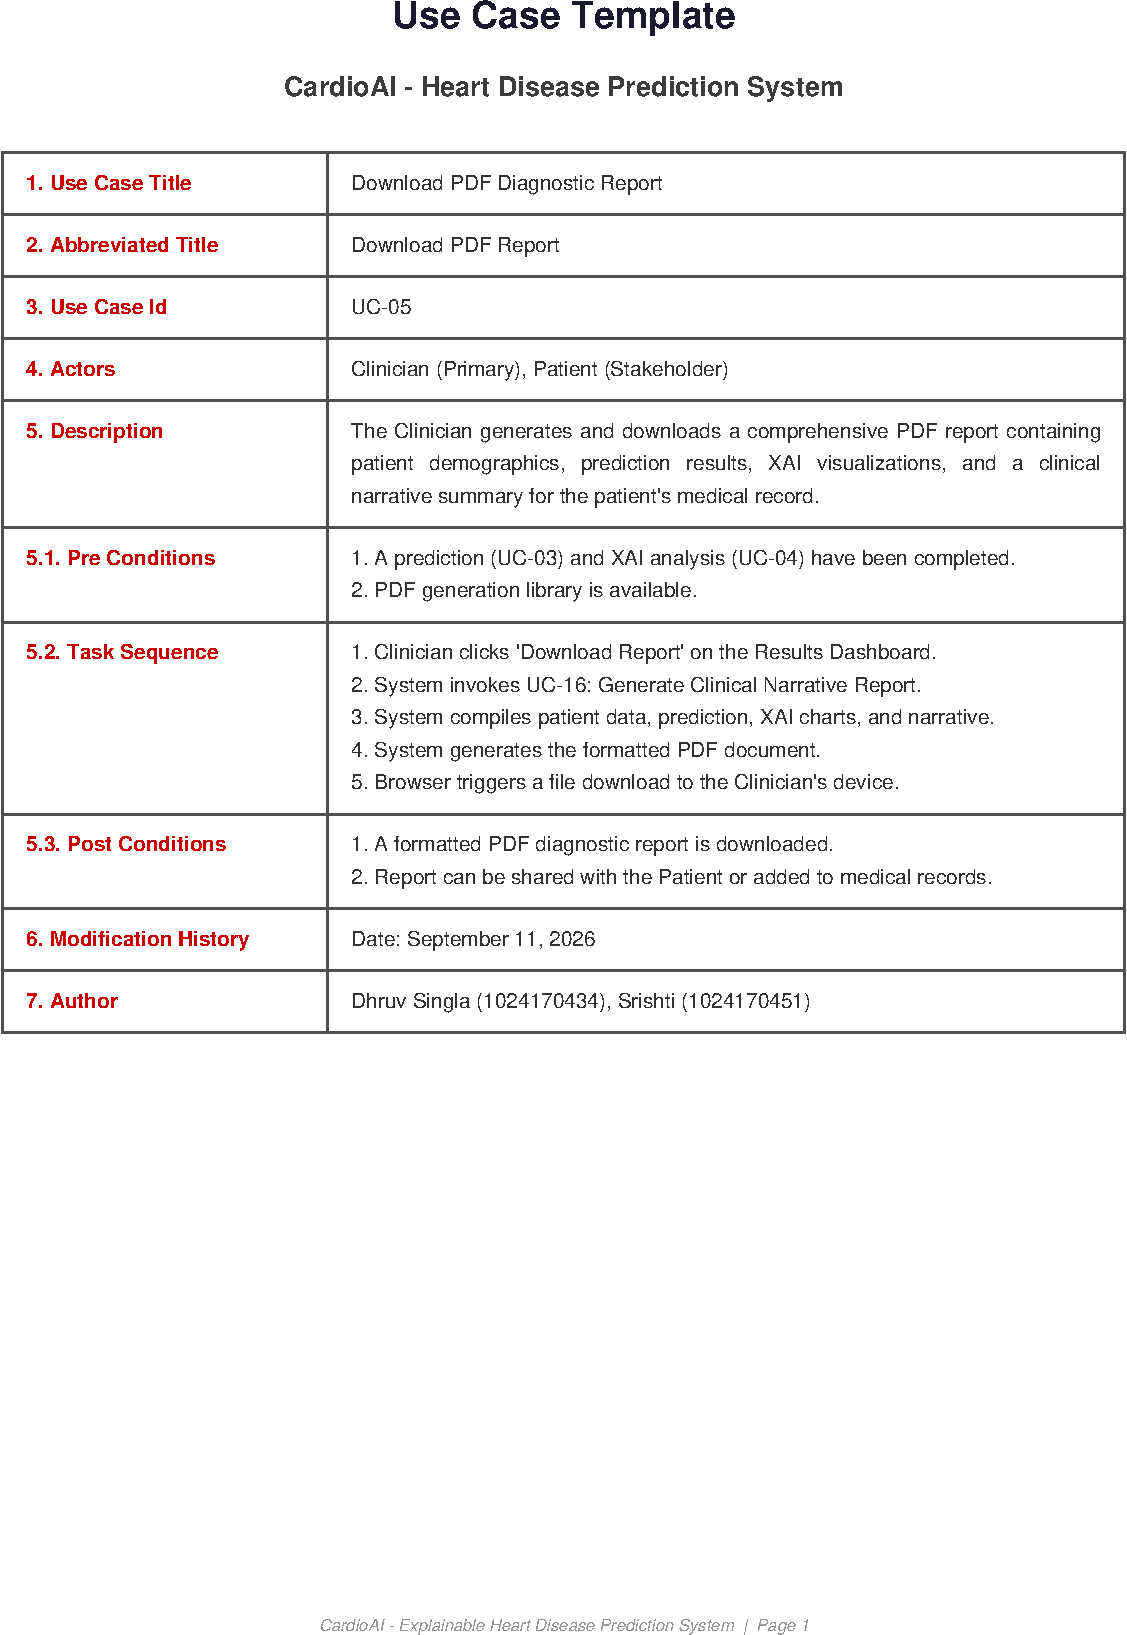
\includegraphics[width=\textwidth,height=0.82\textheight,keepaspectratio]{diagrams/use_case_templates/UC_05_Download_PDF_Report.pdf}
    \caption{Use Case: Download PDF Report}
\end{figure}
\clearpage

\begin{figure}[H]
    \centering
    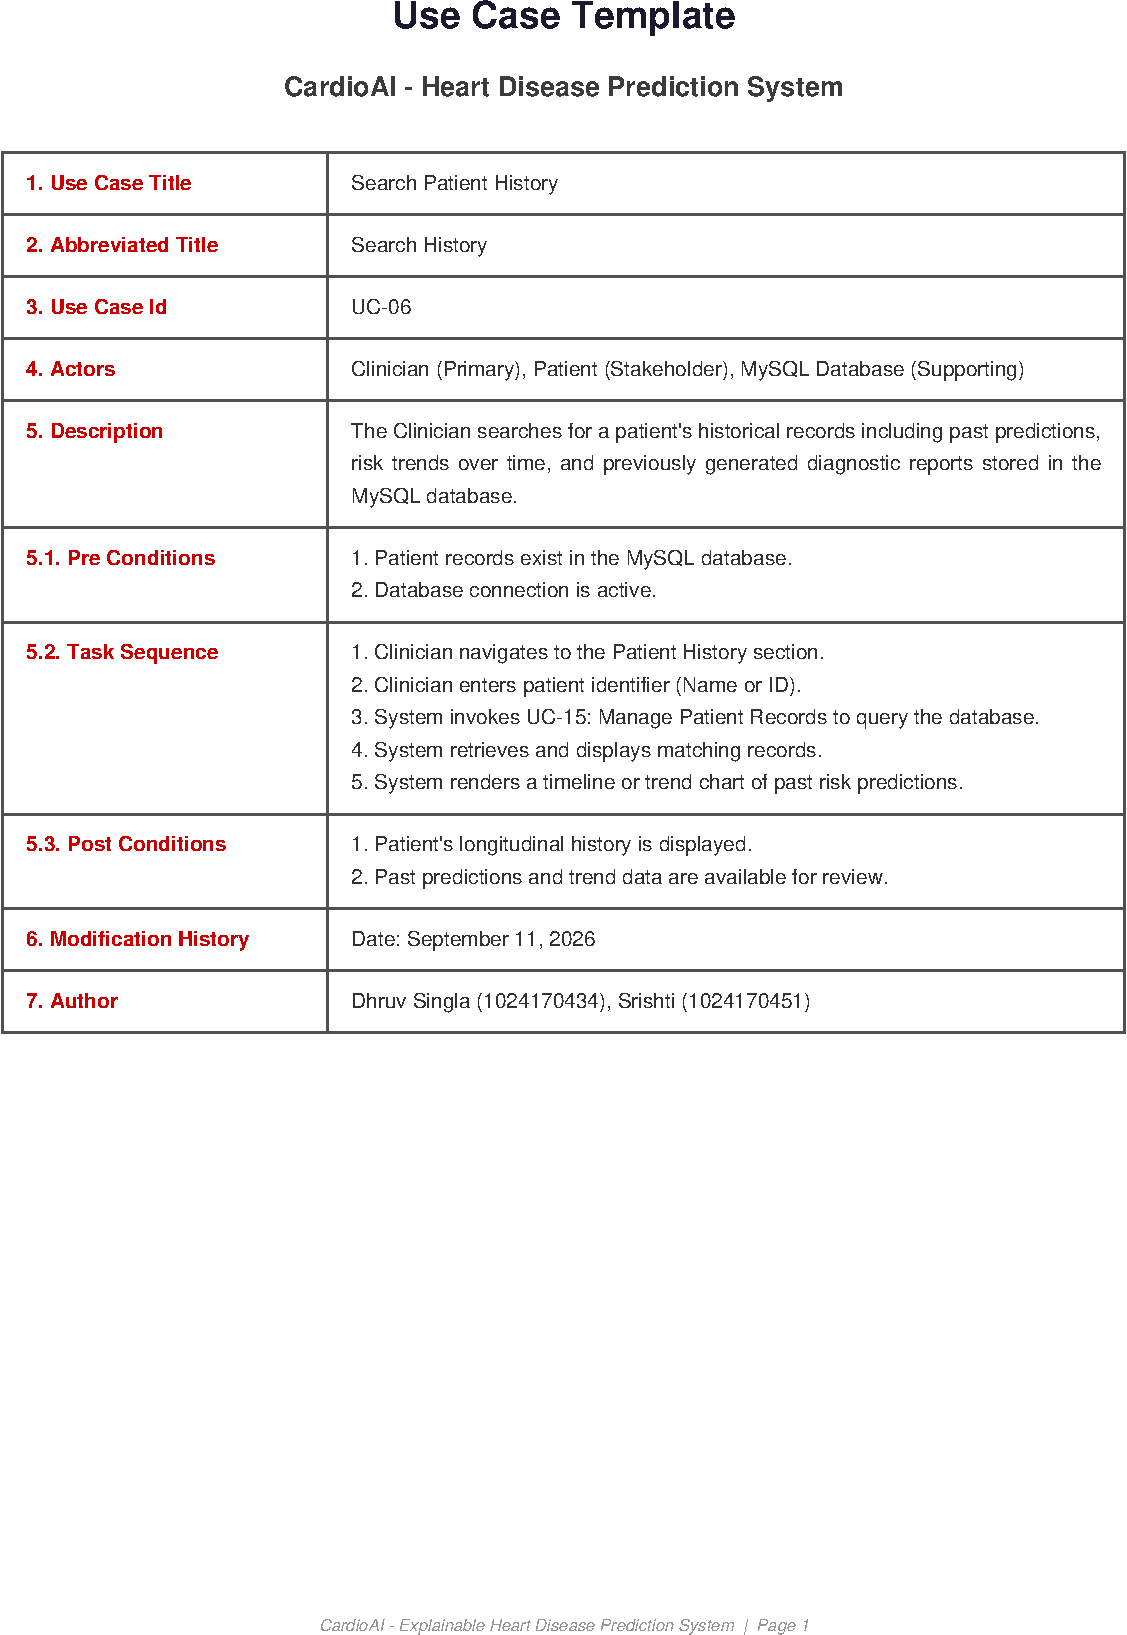
\includegraphics[width=\textwidth,height=0.82\textheight,keepaspectratio]{diagrams/use_case_templates/UC_06_Search_History.pdf}
    \caption{Use Case: Search History}
\end{figure}
\clearpage

\begin{figure}[H]
    \centering
    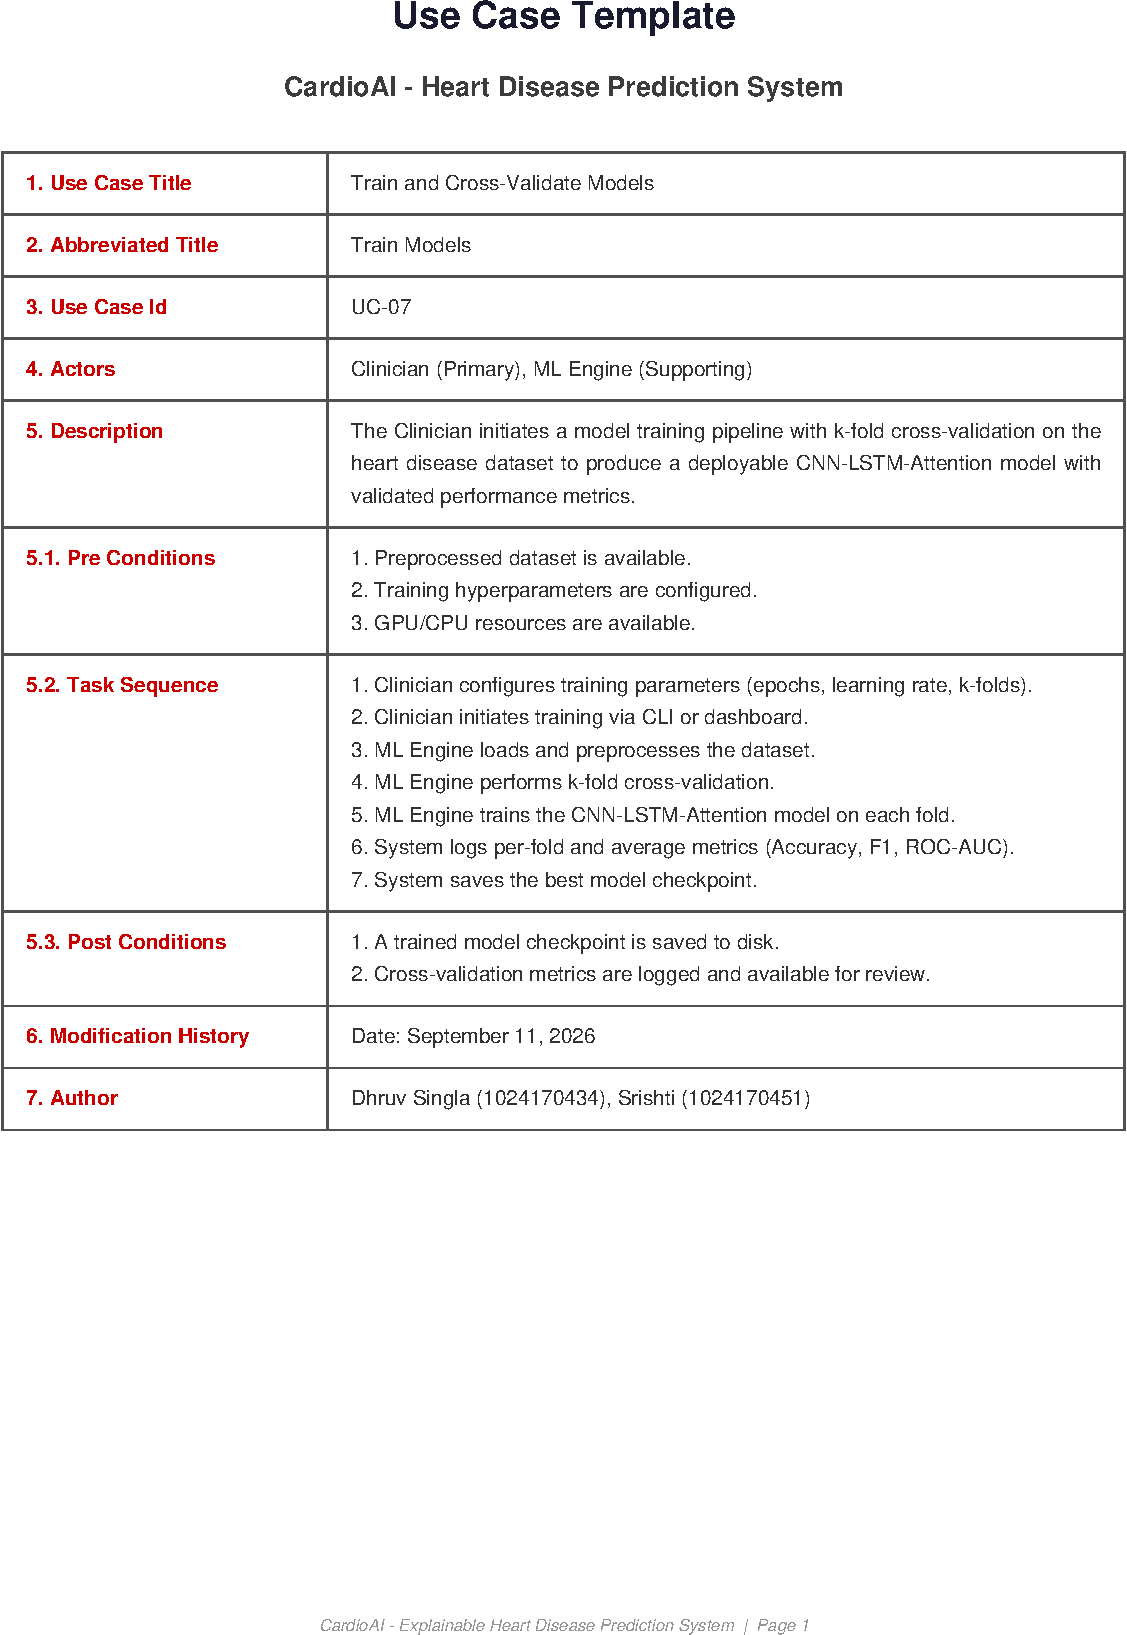
\includegraphics[width=\textwidth,height=0.82\textheight,keepaspectratio]{diagrams/use_case_templates/UC_07_Train_Models.pdf}
    \caption{Use Case: Train Models}
\end{figure}
\clearpage

\begin{figure}[H]
    \centering
    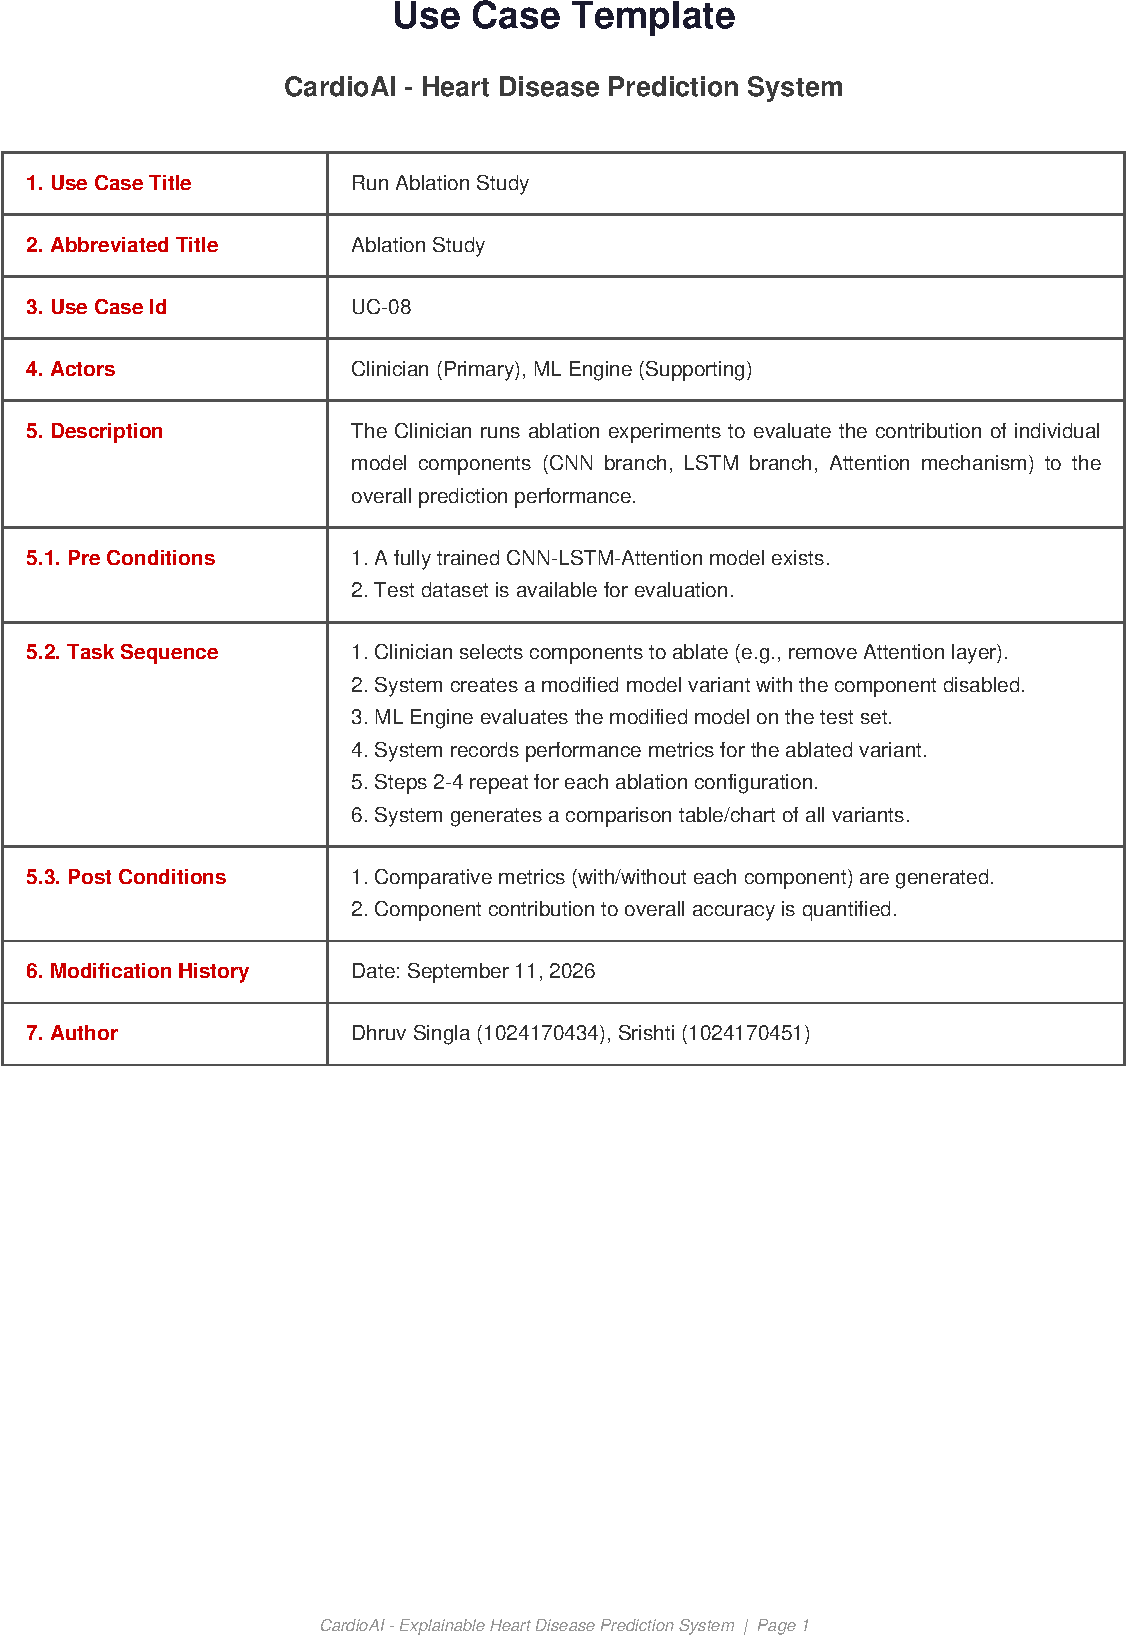
\includegraphics[width=\textwidth,height=0.82\textheight,keepaspectratio]{diagrams/use_case_templates/UC_08_Ablation_Study.pdf}
    \caption{Use Case: Ablation Study}
\end{figure}
\clearpage

\begin{figure}[H]
    \centering
    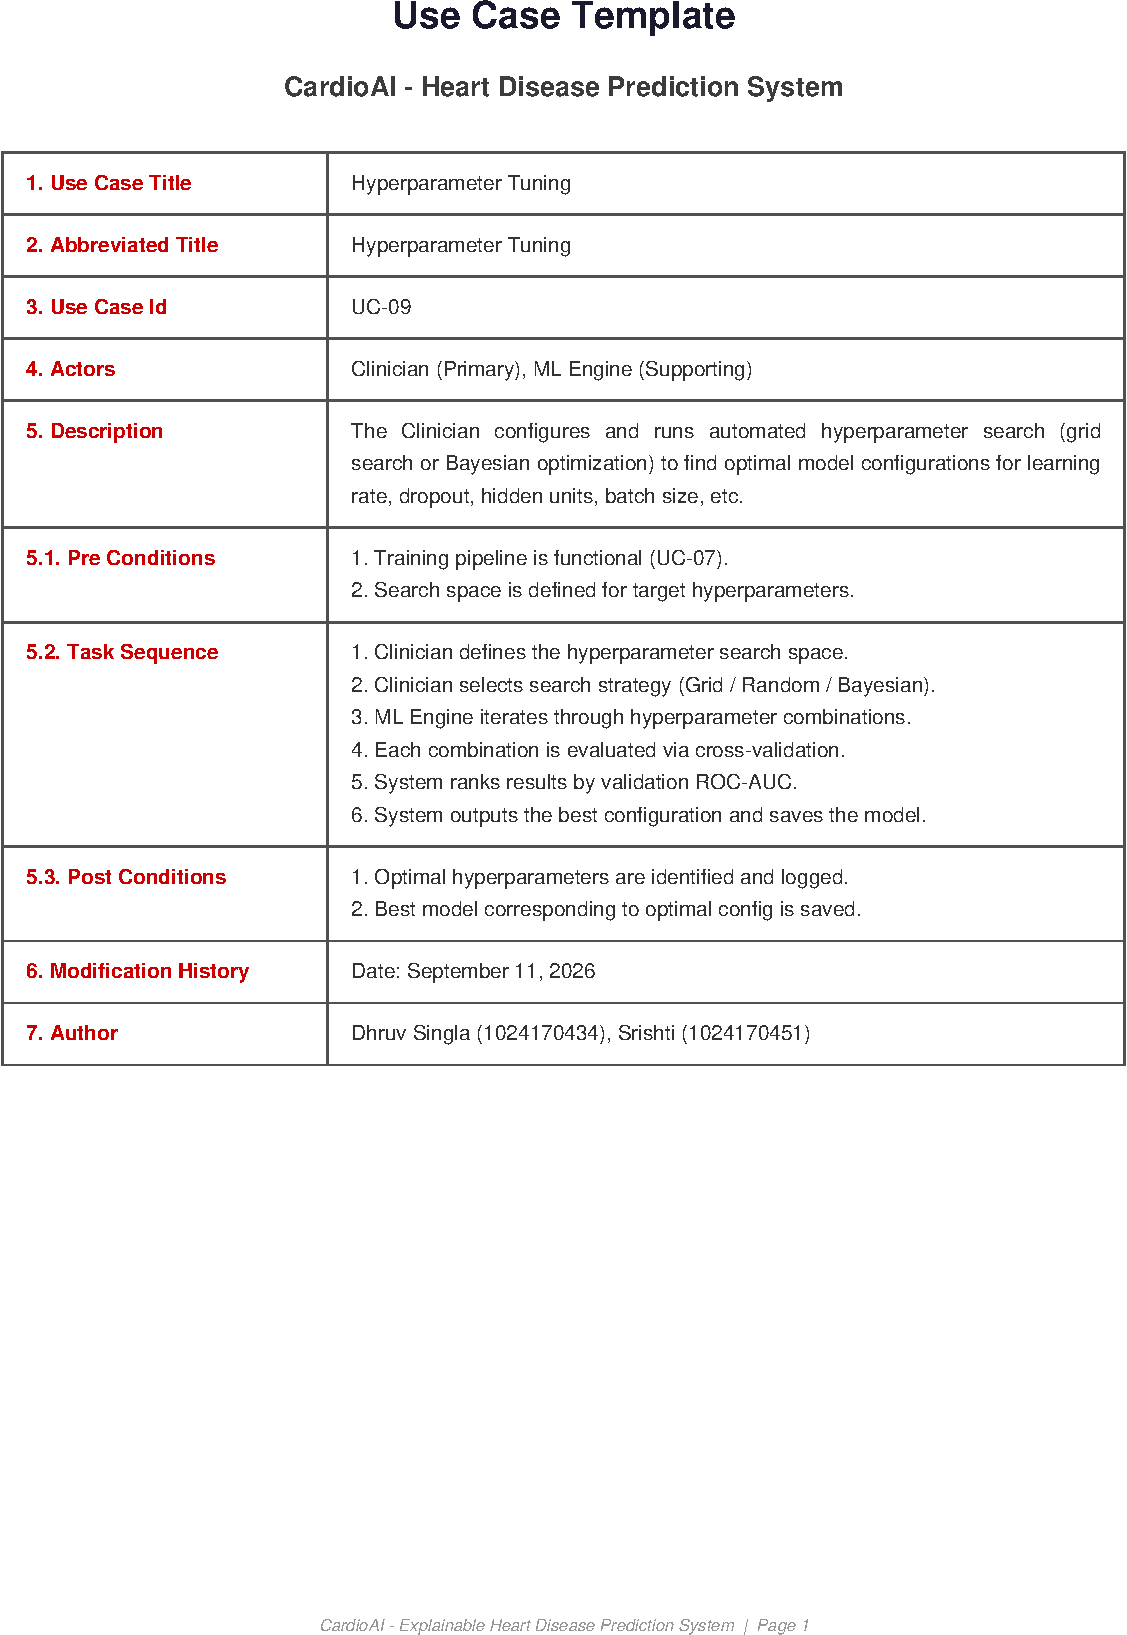
\includegraphics[width=\textwidth,height=0.82\textheight,keepaspectratio]{diagrams/use_case_templates/UC_09_Hyperparameter_Tuning.pdf}
    \caption{Use Case: Hyperparameter Tuning}
\end{figure}
\clearpage

\begin{figure}[H]
    \centering
    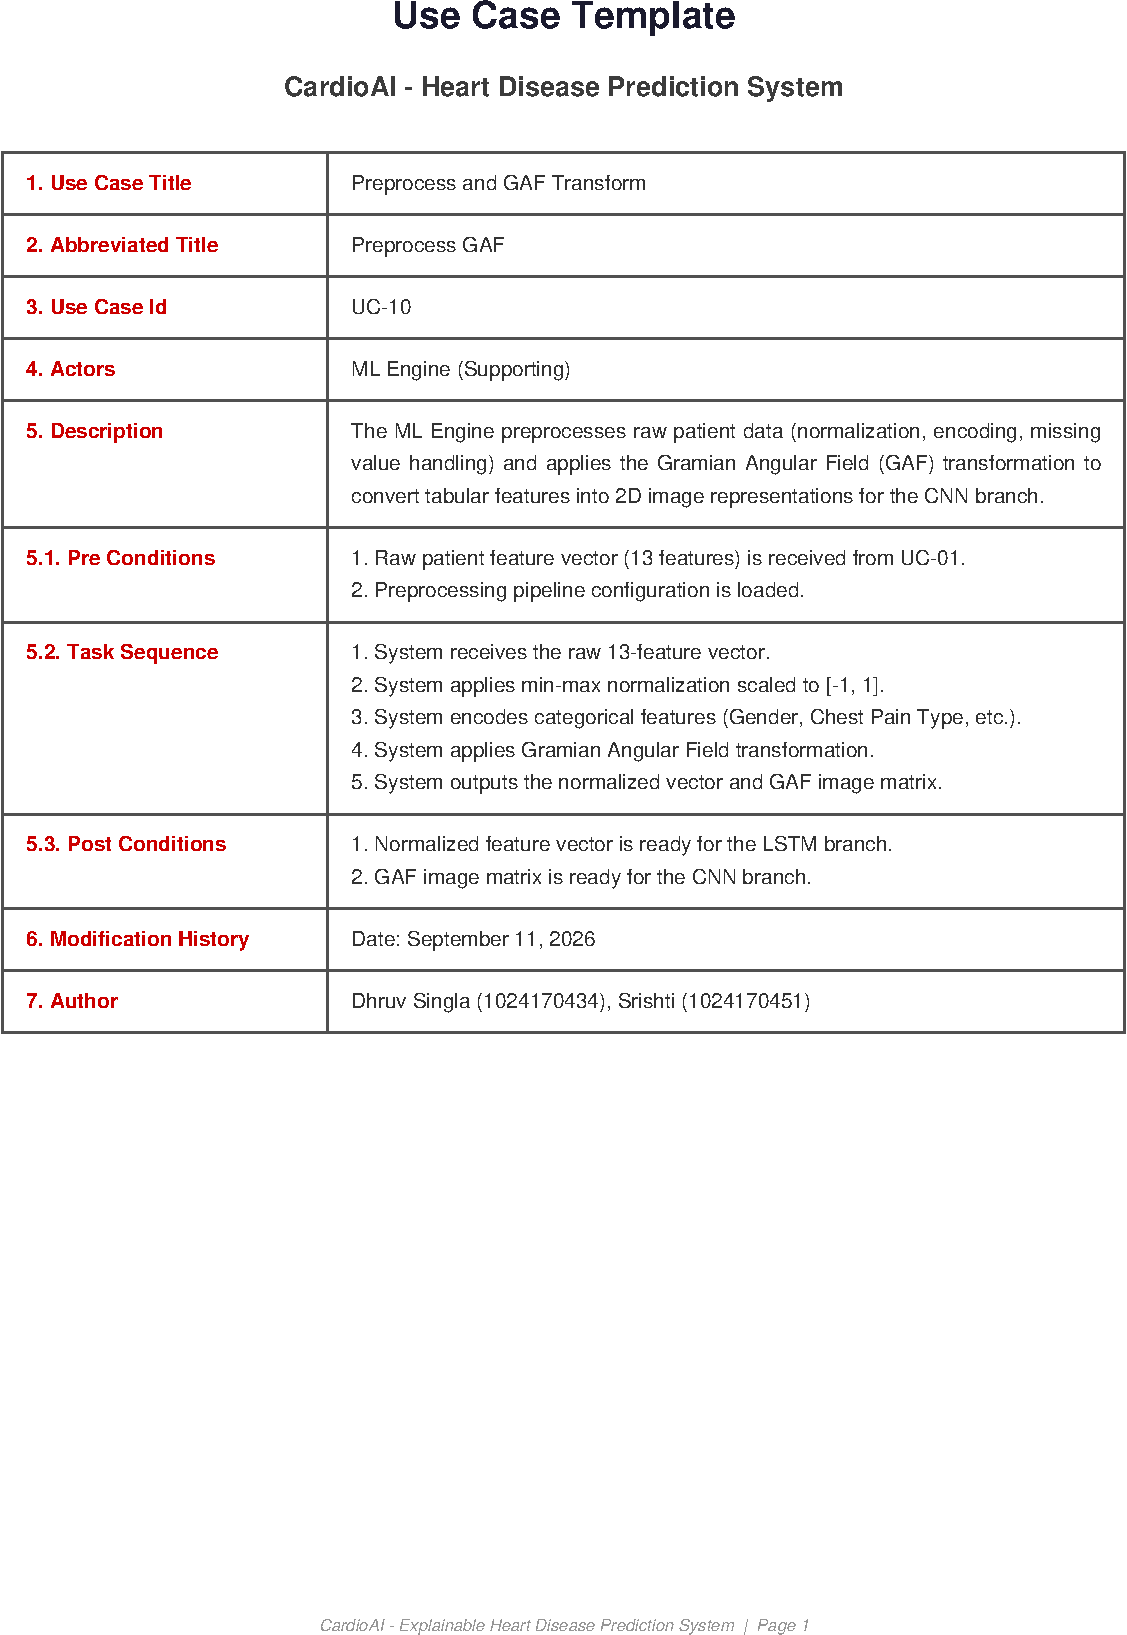
\includegraphics[width=\textwidth,height=0.82\textheight,keepaspectratio]{diagrams/use_case_templates/UC_10_Preprocess_GAF.pdf}
    \caption{Use Case: Preprocess GAF}
\end{figure}
\clearpage

\begin{figure}[H]
    \centering
    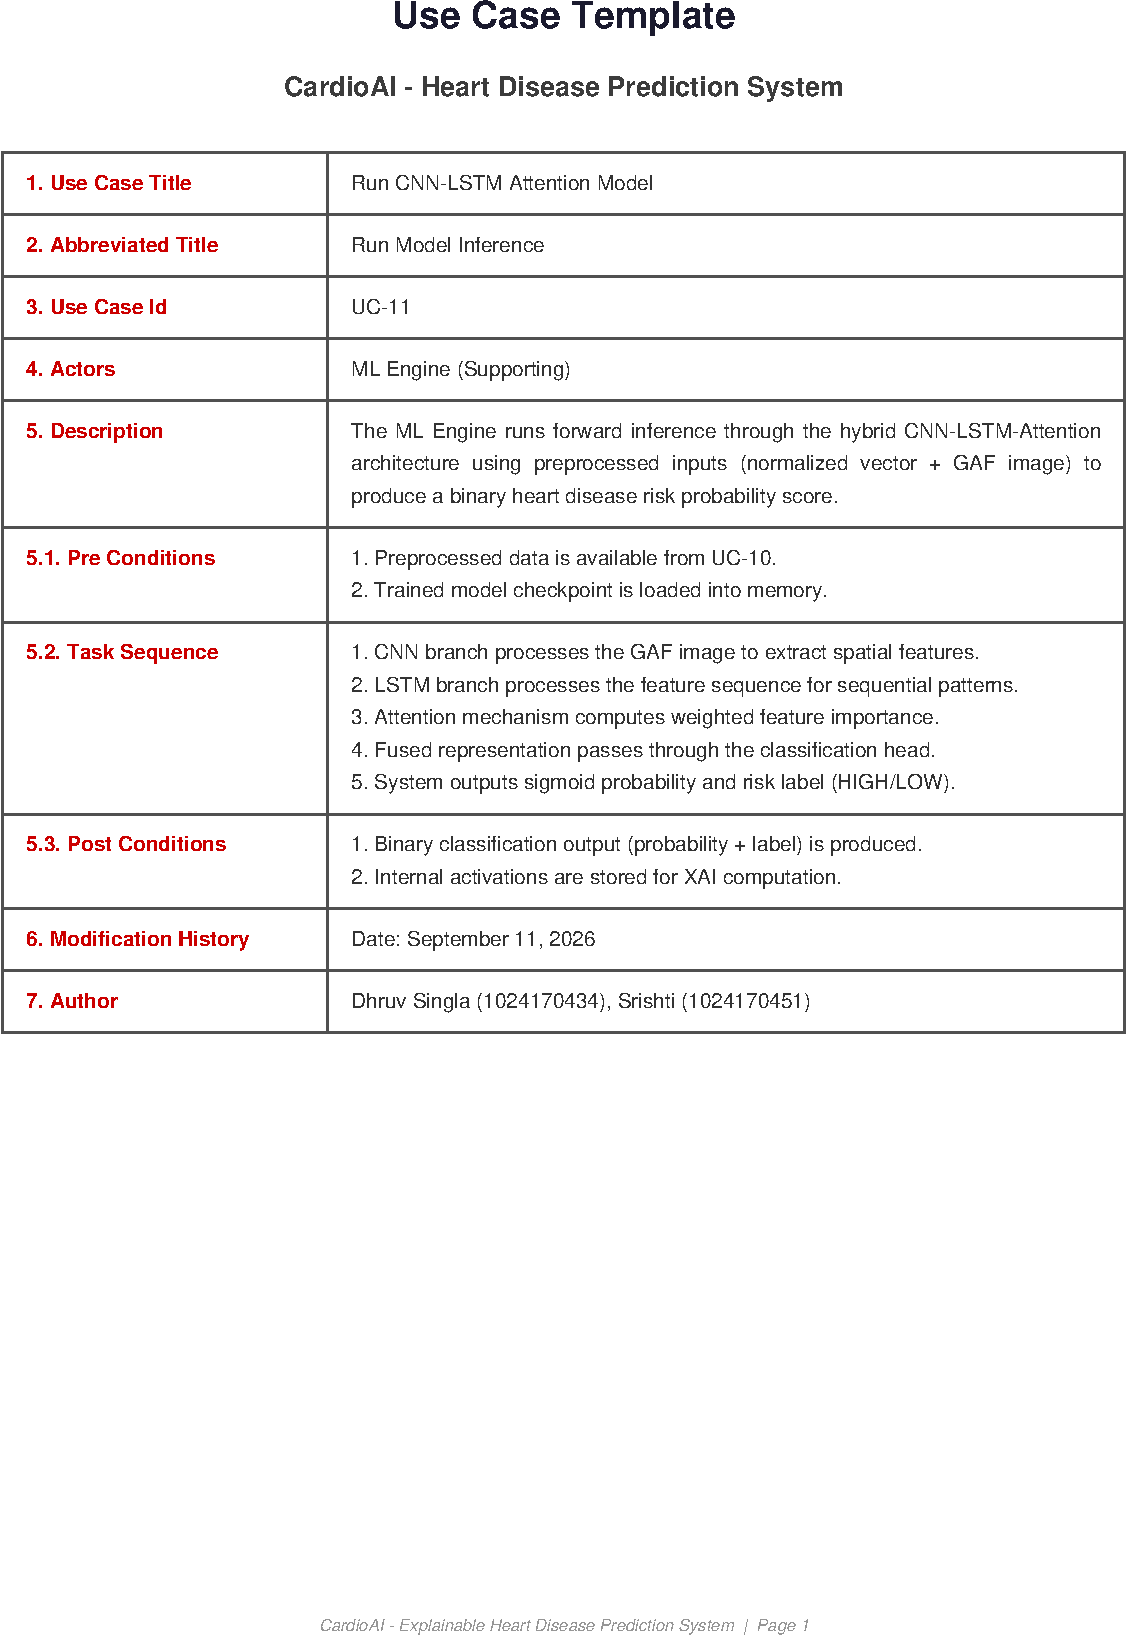
\includegraphics[width=\textwidth,height=0.82\textheight,keepaspectratio]{diagrams/use_case_templates/UC_11_Run_Model_Inference.pdf}
    \caption{Use Case: Run Model Inference}
\end{figure}
\clearpage

\begin{figure}[H]
    \centering
    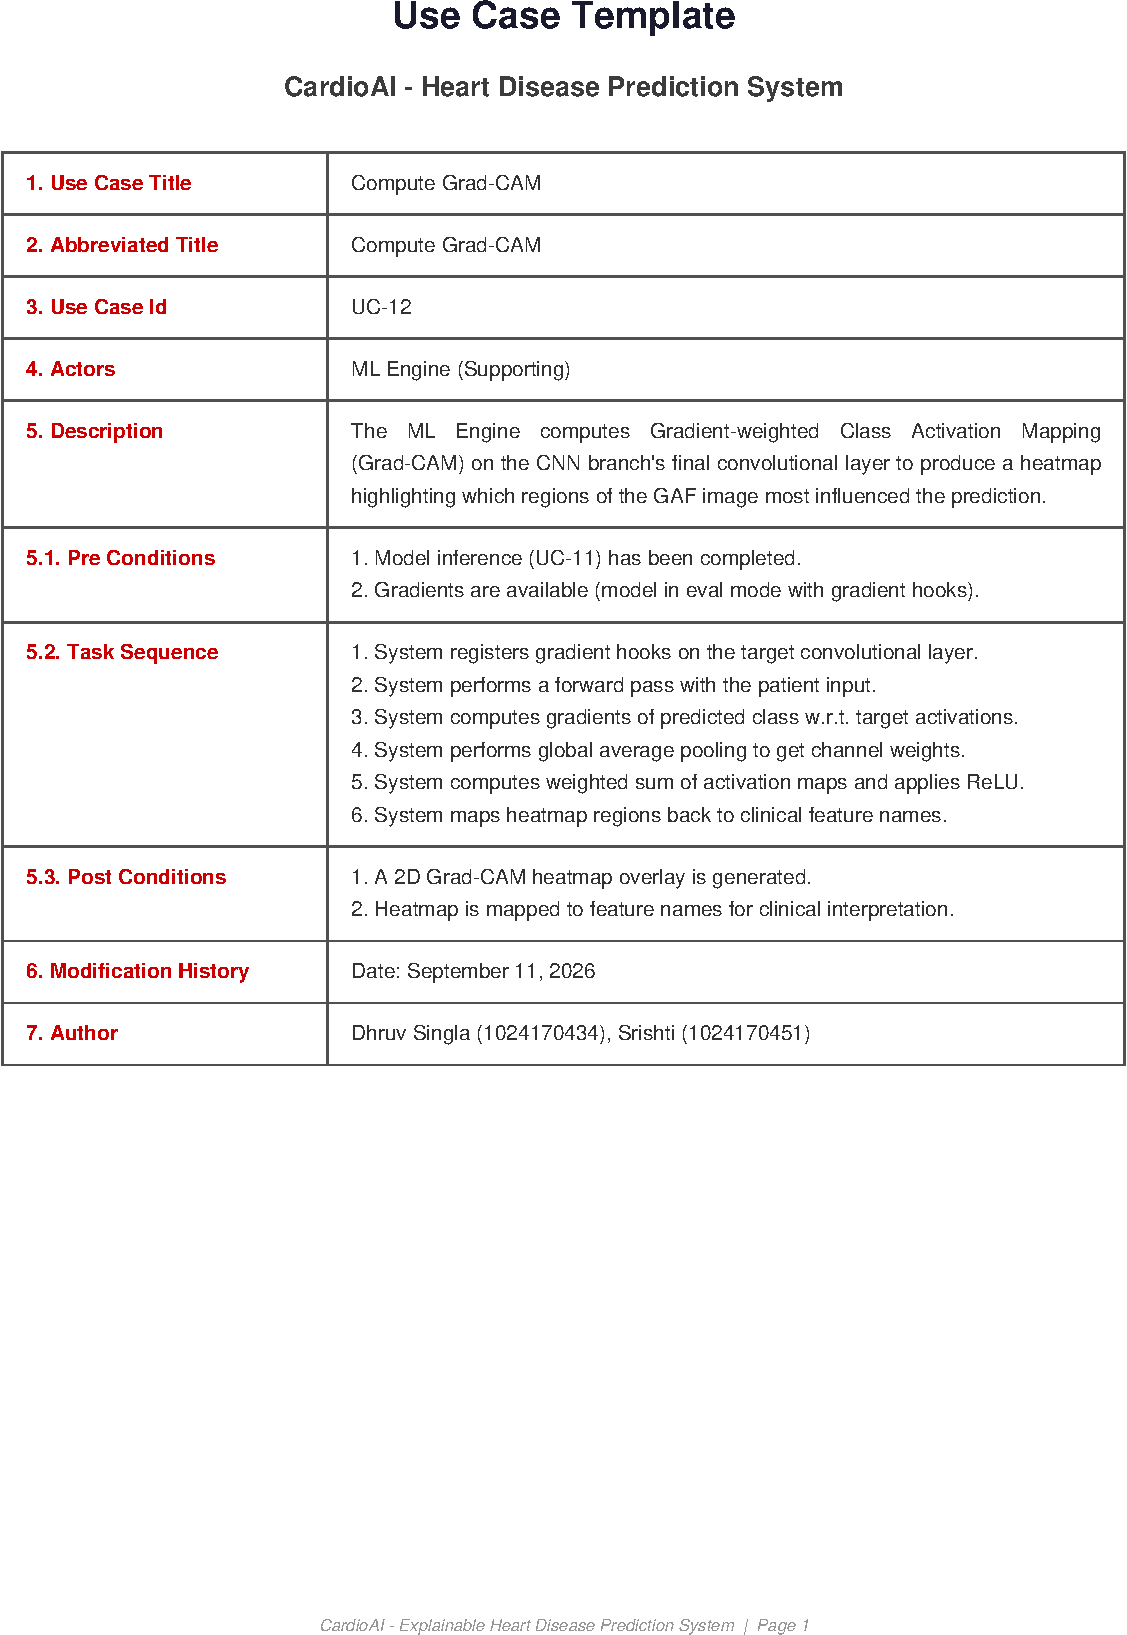
\includegraphics[width=\textwidth,height=0.82\textheight,keepaspectratio]{diagrams/use_case_templates/UC_12_Compute_Grad-CAM.pdf}
    \caption{Use Case: Compute Grad-CAM}
\end{figure}
\clearpage

\begin{figure}[H]
    \centering
    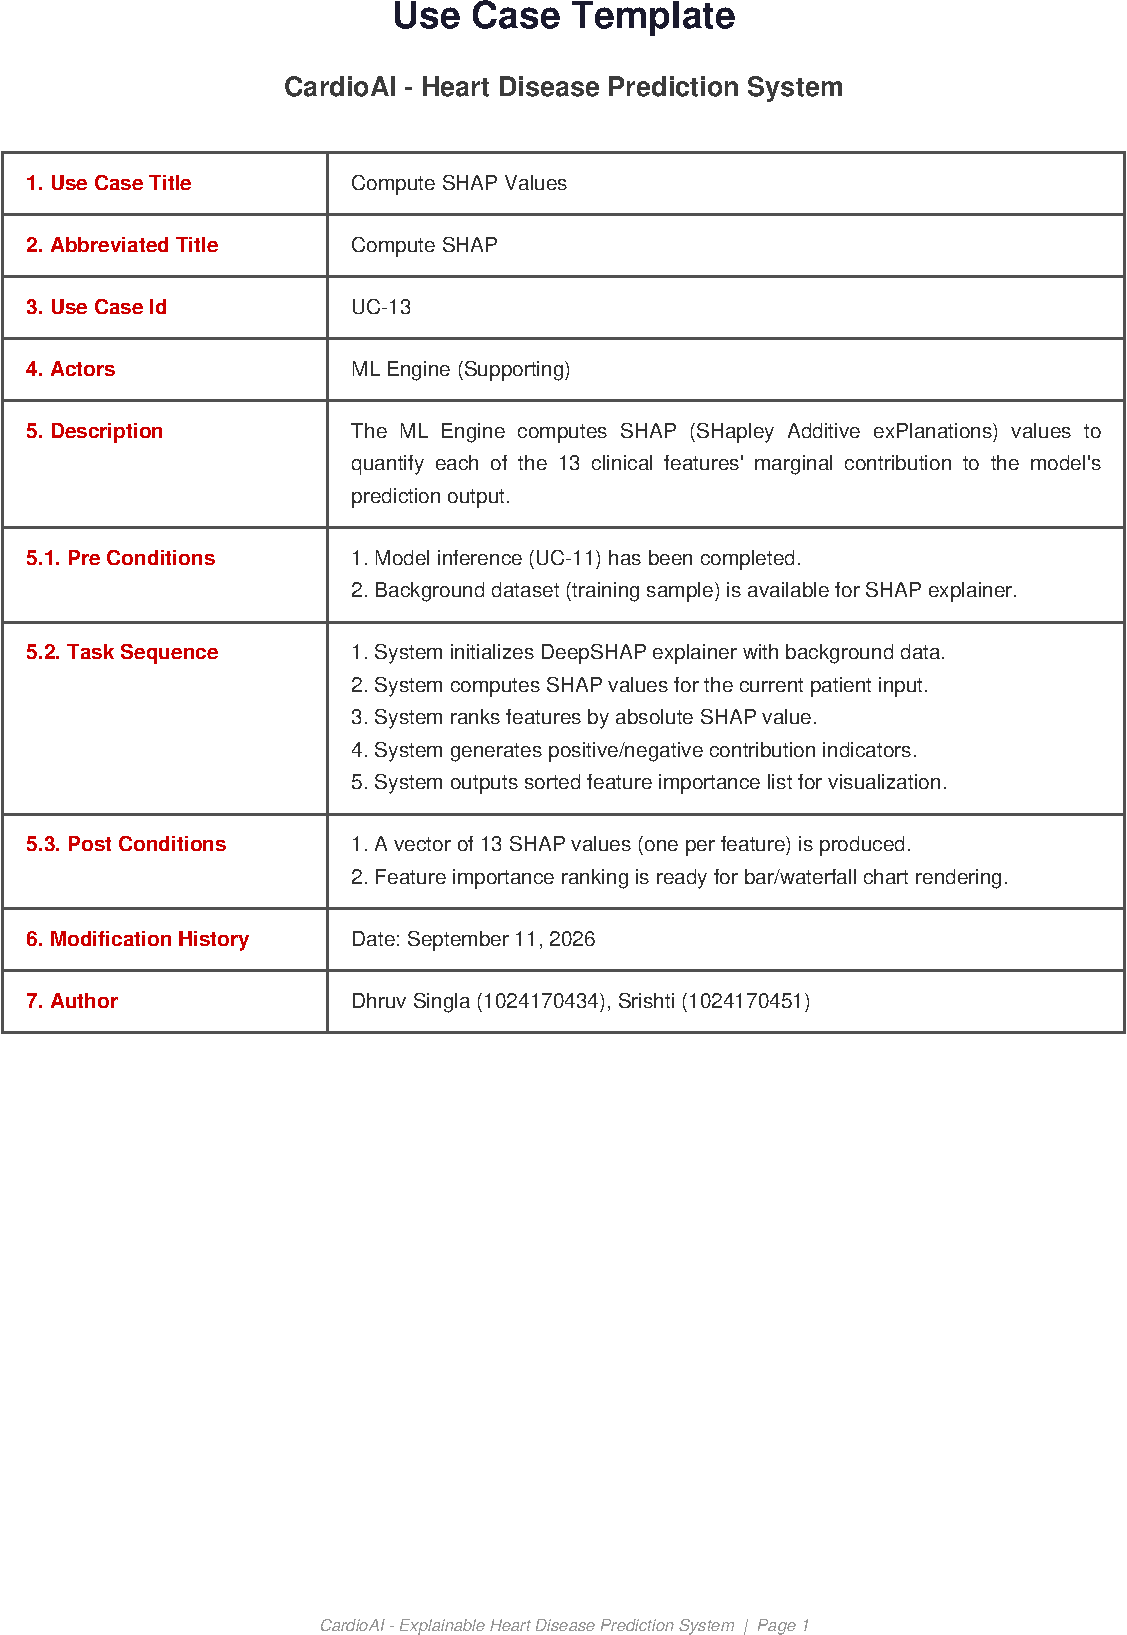
\includegraphics[width=\textwidth,height=0.82\textheight,keepaspectratio]{diagrams/use_case_templates/UC_13_Compute_SHAP.pdf}
    \caption{Use Case: Compute SHAP}
\end{figure}
\clearpage

\begin{figure}[H]
    \centering
    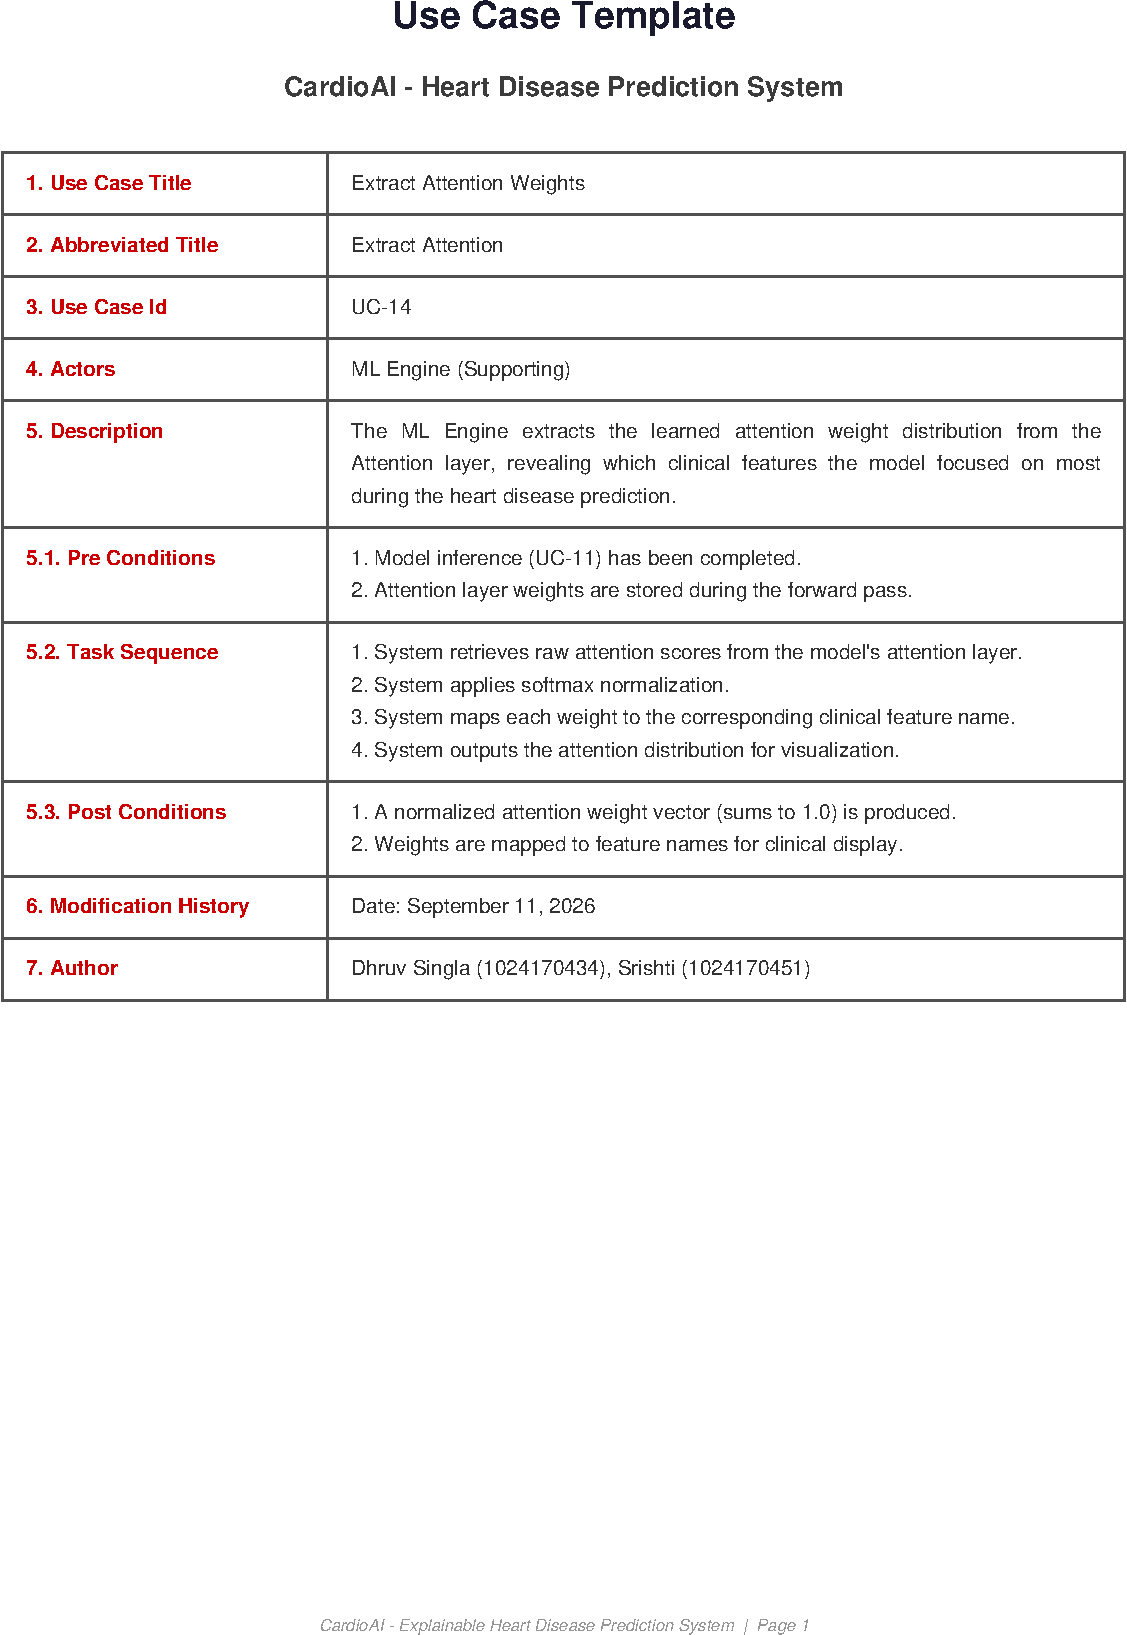
\includegraphics[width=\textwidth,height=0.82\textheight,keepaspectratio]{diagrams/use_case_templates/UC_14_Extract_Attention.pdf}
    \caption{Use Case: Extract Attention}
\end{figure}
\clearpage

\begin{figure}[H]
    \centering
    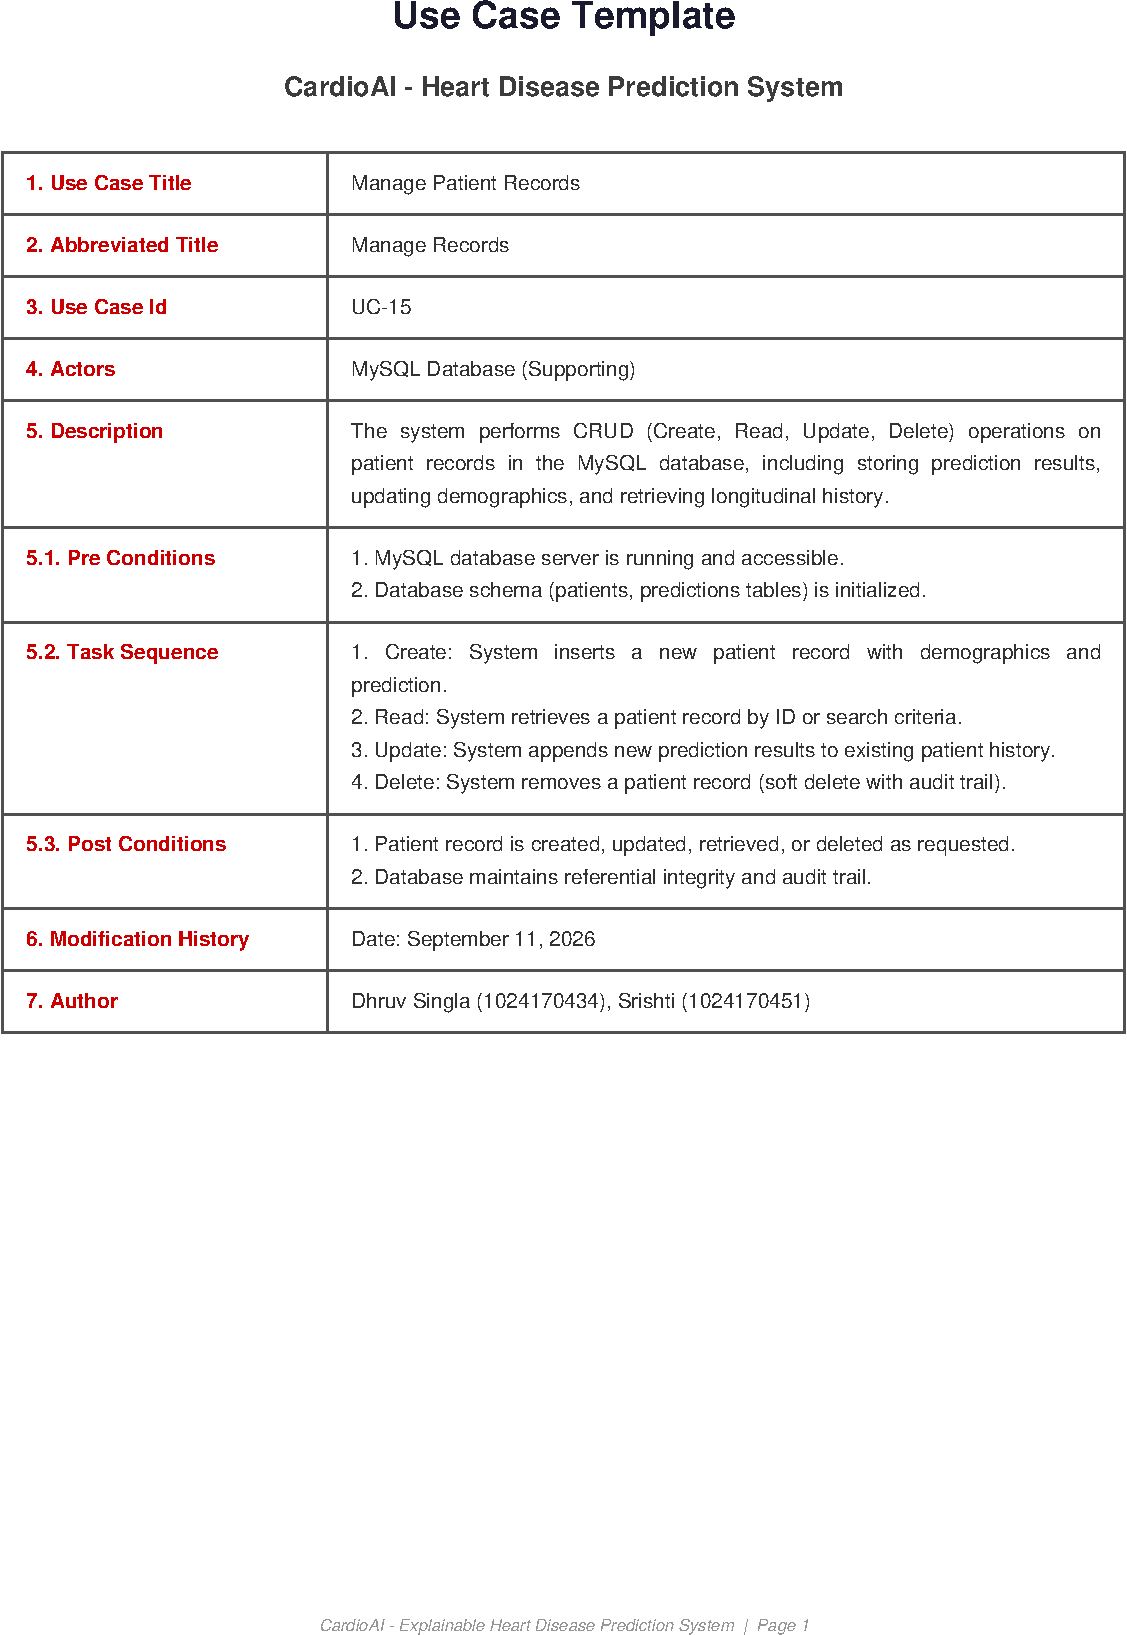
\includegraphics[width=\textwidth,height=0.82\textheight,keepaspectratio]{diagrams/use_case_templates/UC_15_Manage_Records.pdf}
    \caption{Use Case: Manage Records}
\end{figure}
\clearpage

\begin{figure}[H]
    \centering
    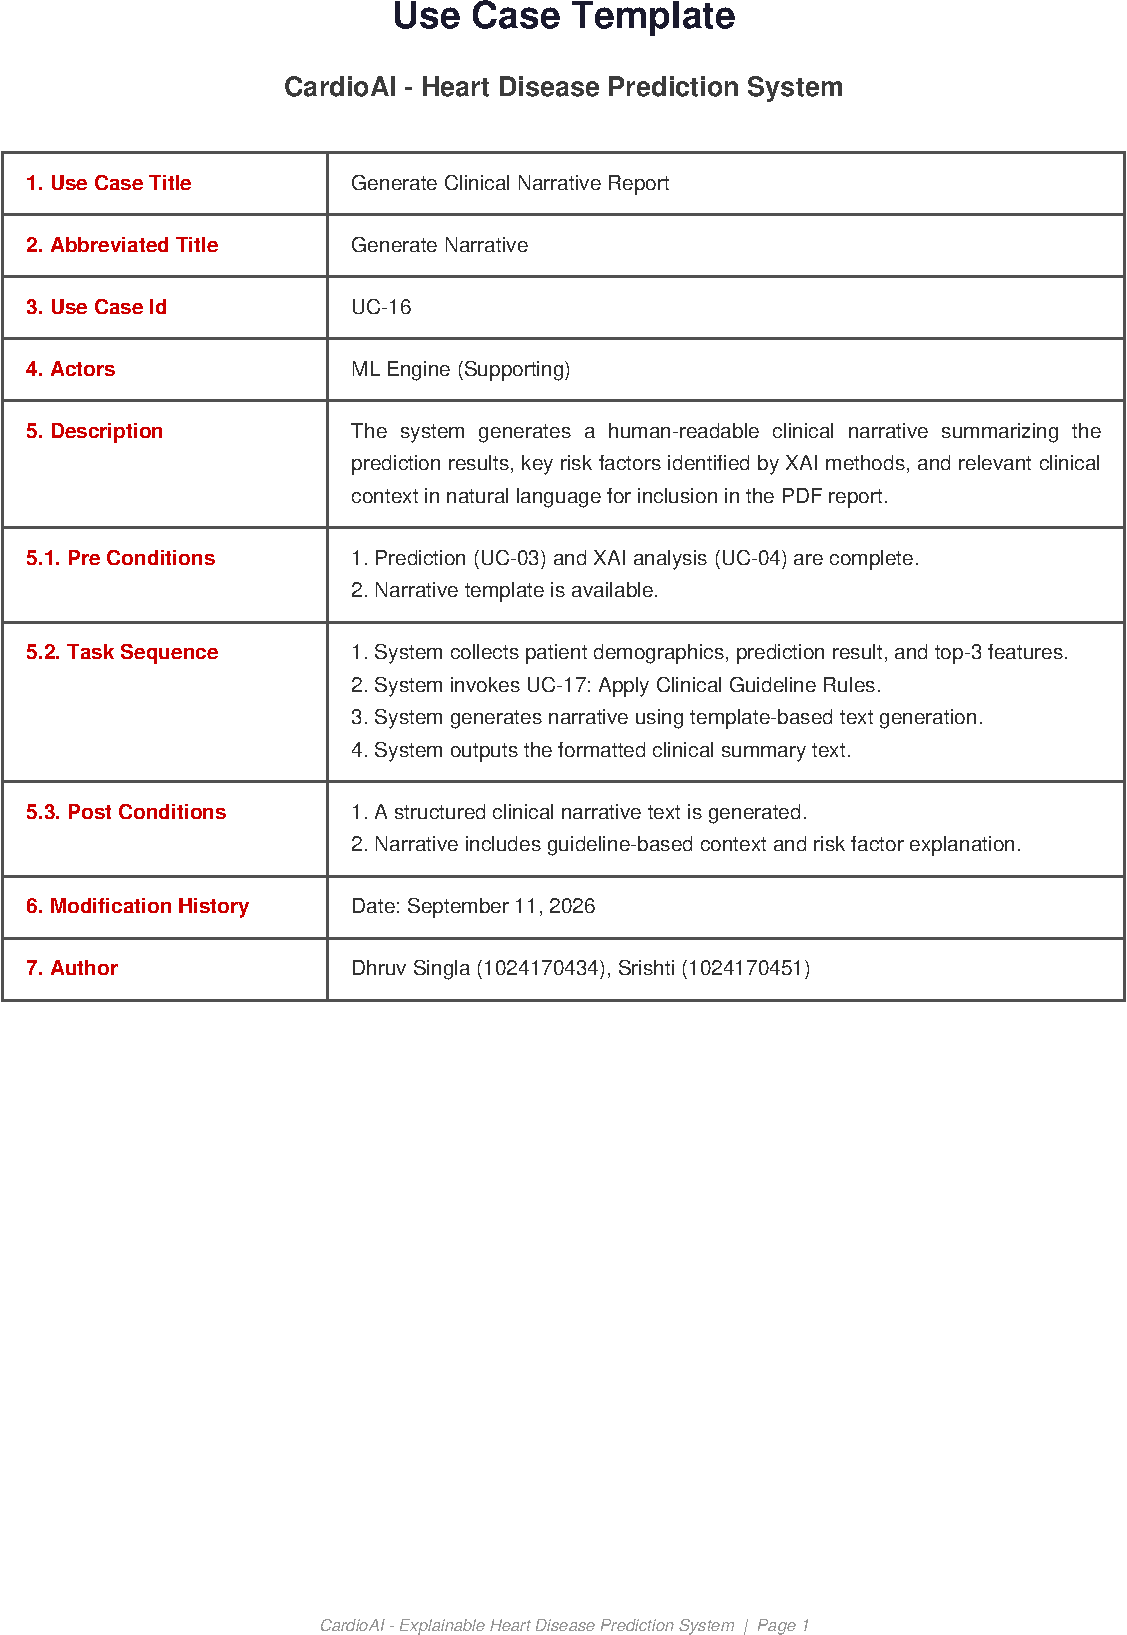
\includegraphics[width=\textwidth,height=0.82\textheight,keepaspectratio]{diagrams/use_case_templates/UC_16_Generate_Narrative.pdf}
    \caption{Use Case: Generate Narrative}
\end{figure}
\clearpage

\begin{figure}[H]
    \centering
    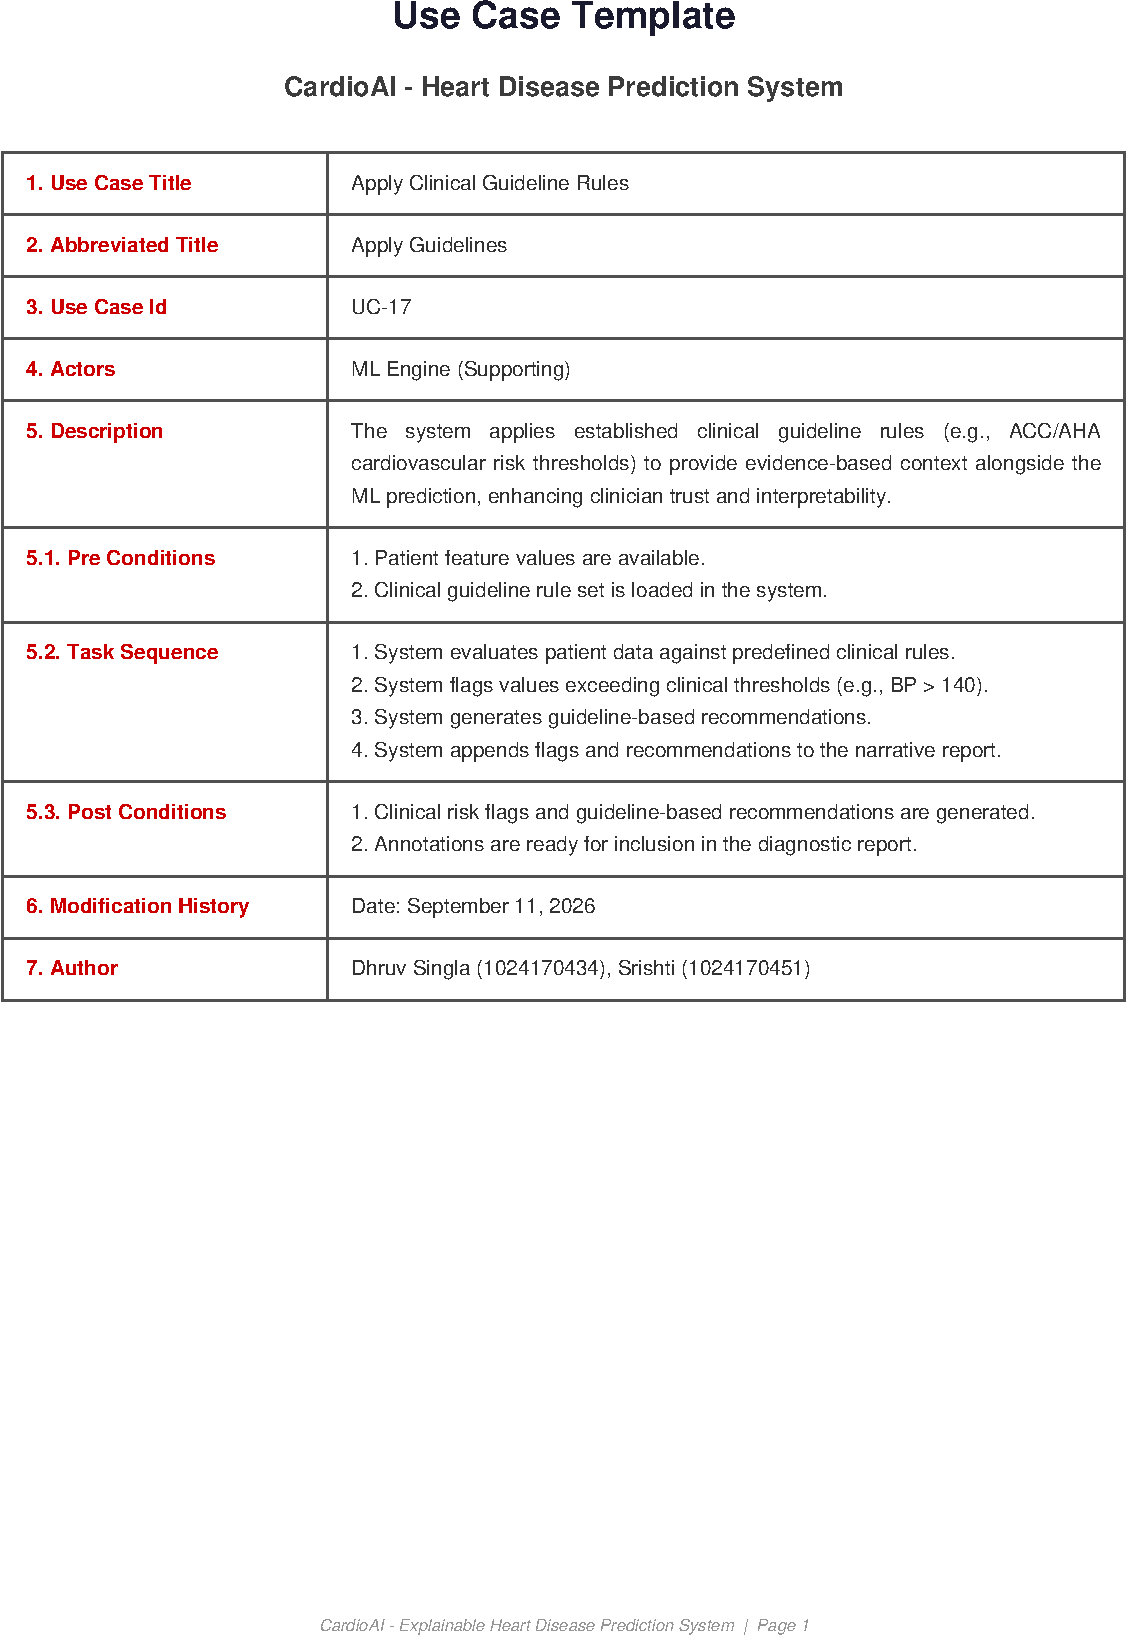
\includegraphics[width=\textwidth,height=0.82\textheight,keepaspectratio]{diagrams/use_case_templates/UC_17_Apply_Guidelines.pdf}
    \caption{Use Case: Apply Guidelines}
\end{figure}
\clearpage

\begin{figure}[H]
    \centering
    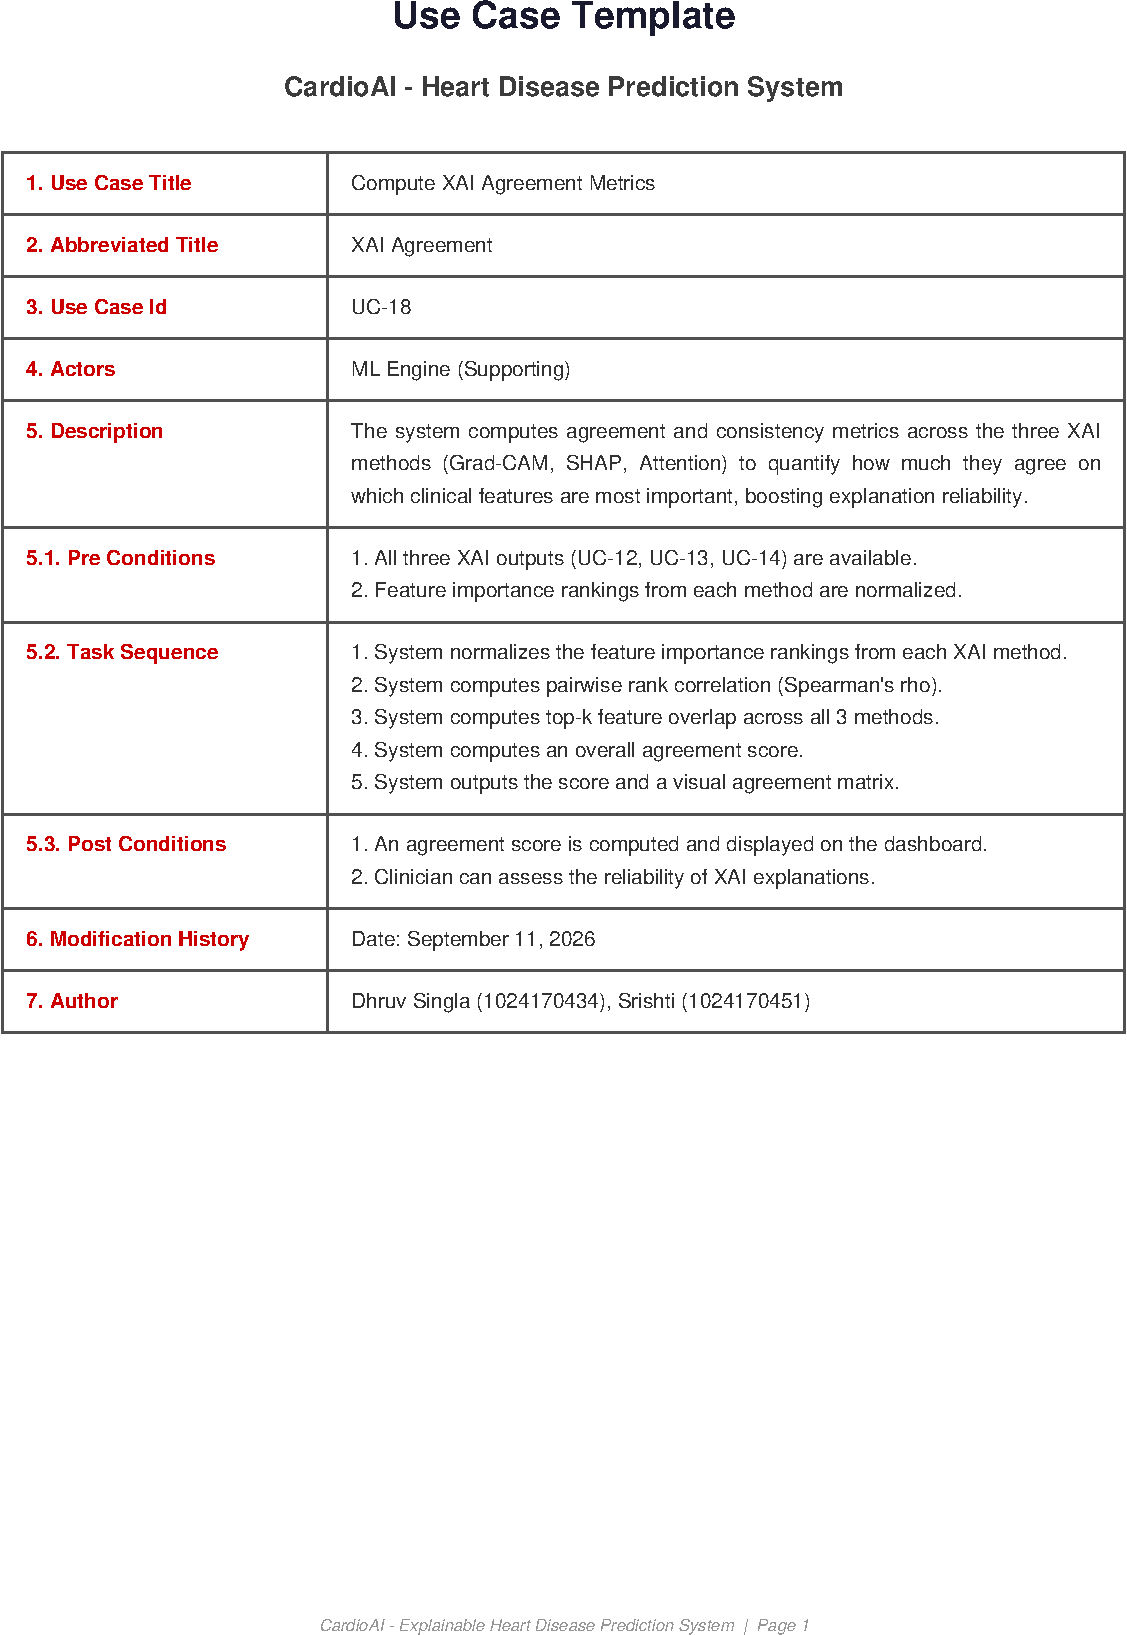
\includegraphics[width=\textwidth,height=0.82\textheight,keepaspectratio]{diagrams/use_case_templates/UC_18_XAI_Agreement.pdf}
    \caption{Use Case: XAI Agreement}
\end{figure}
\clearpage

\subsection{UML Activity Diagram}
\begin{figure}[H]
    \centering
    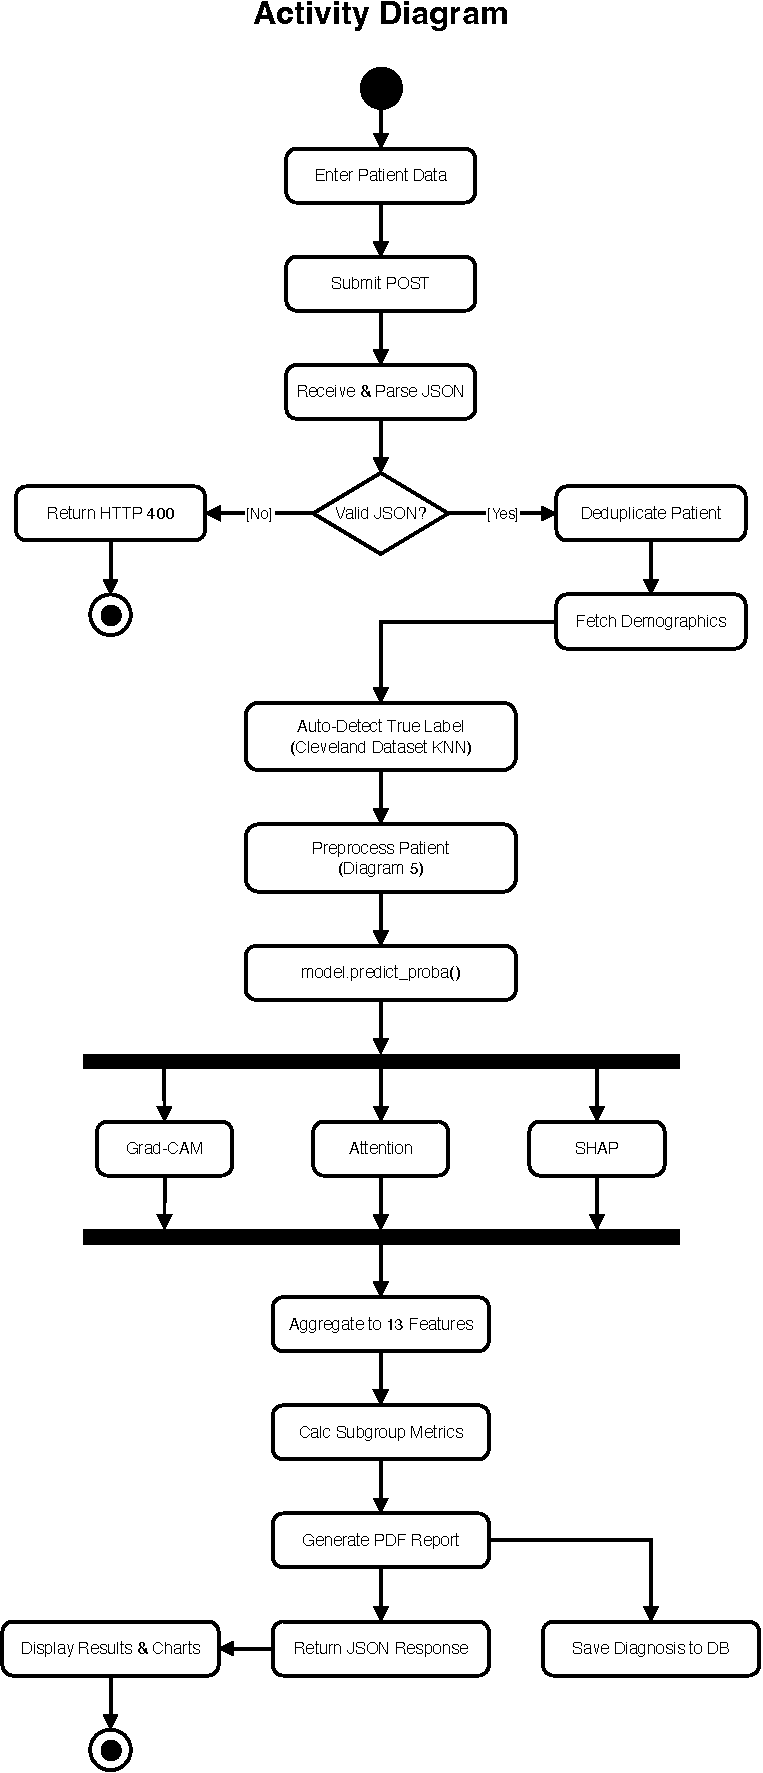
\includegraphics[width=\textwidth,height=0.82\textheight,keepaspectratio]{diagrams/activity diagram.pdf}
    \caption{UML Activity Diagram mapping the procedural flow of the system.}
    \label{fig:activity}
\end{figure}

\clearpage
\subsection{UML Activity Diagram (Swimlanes)}
\begin{figure}[H]
    \centering
    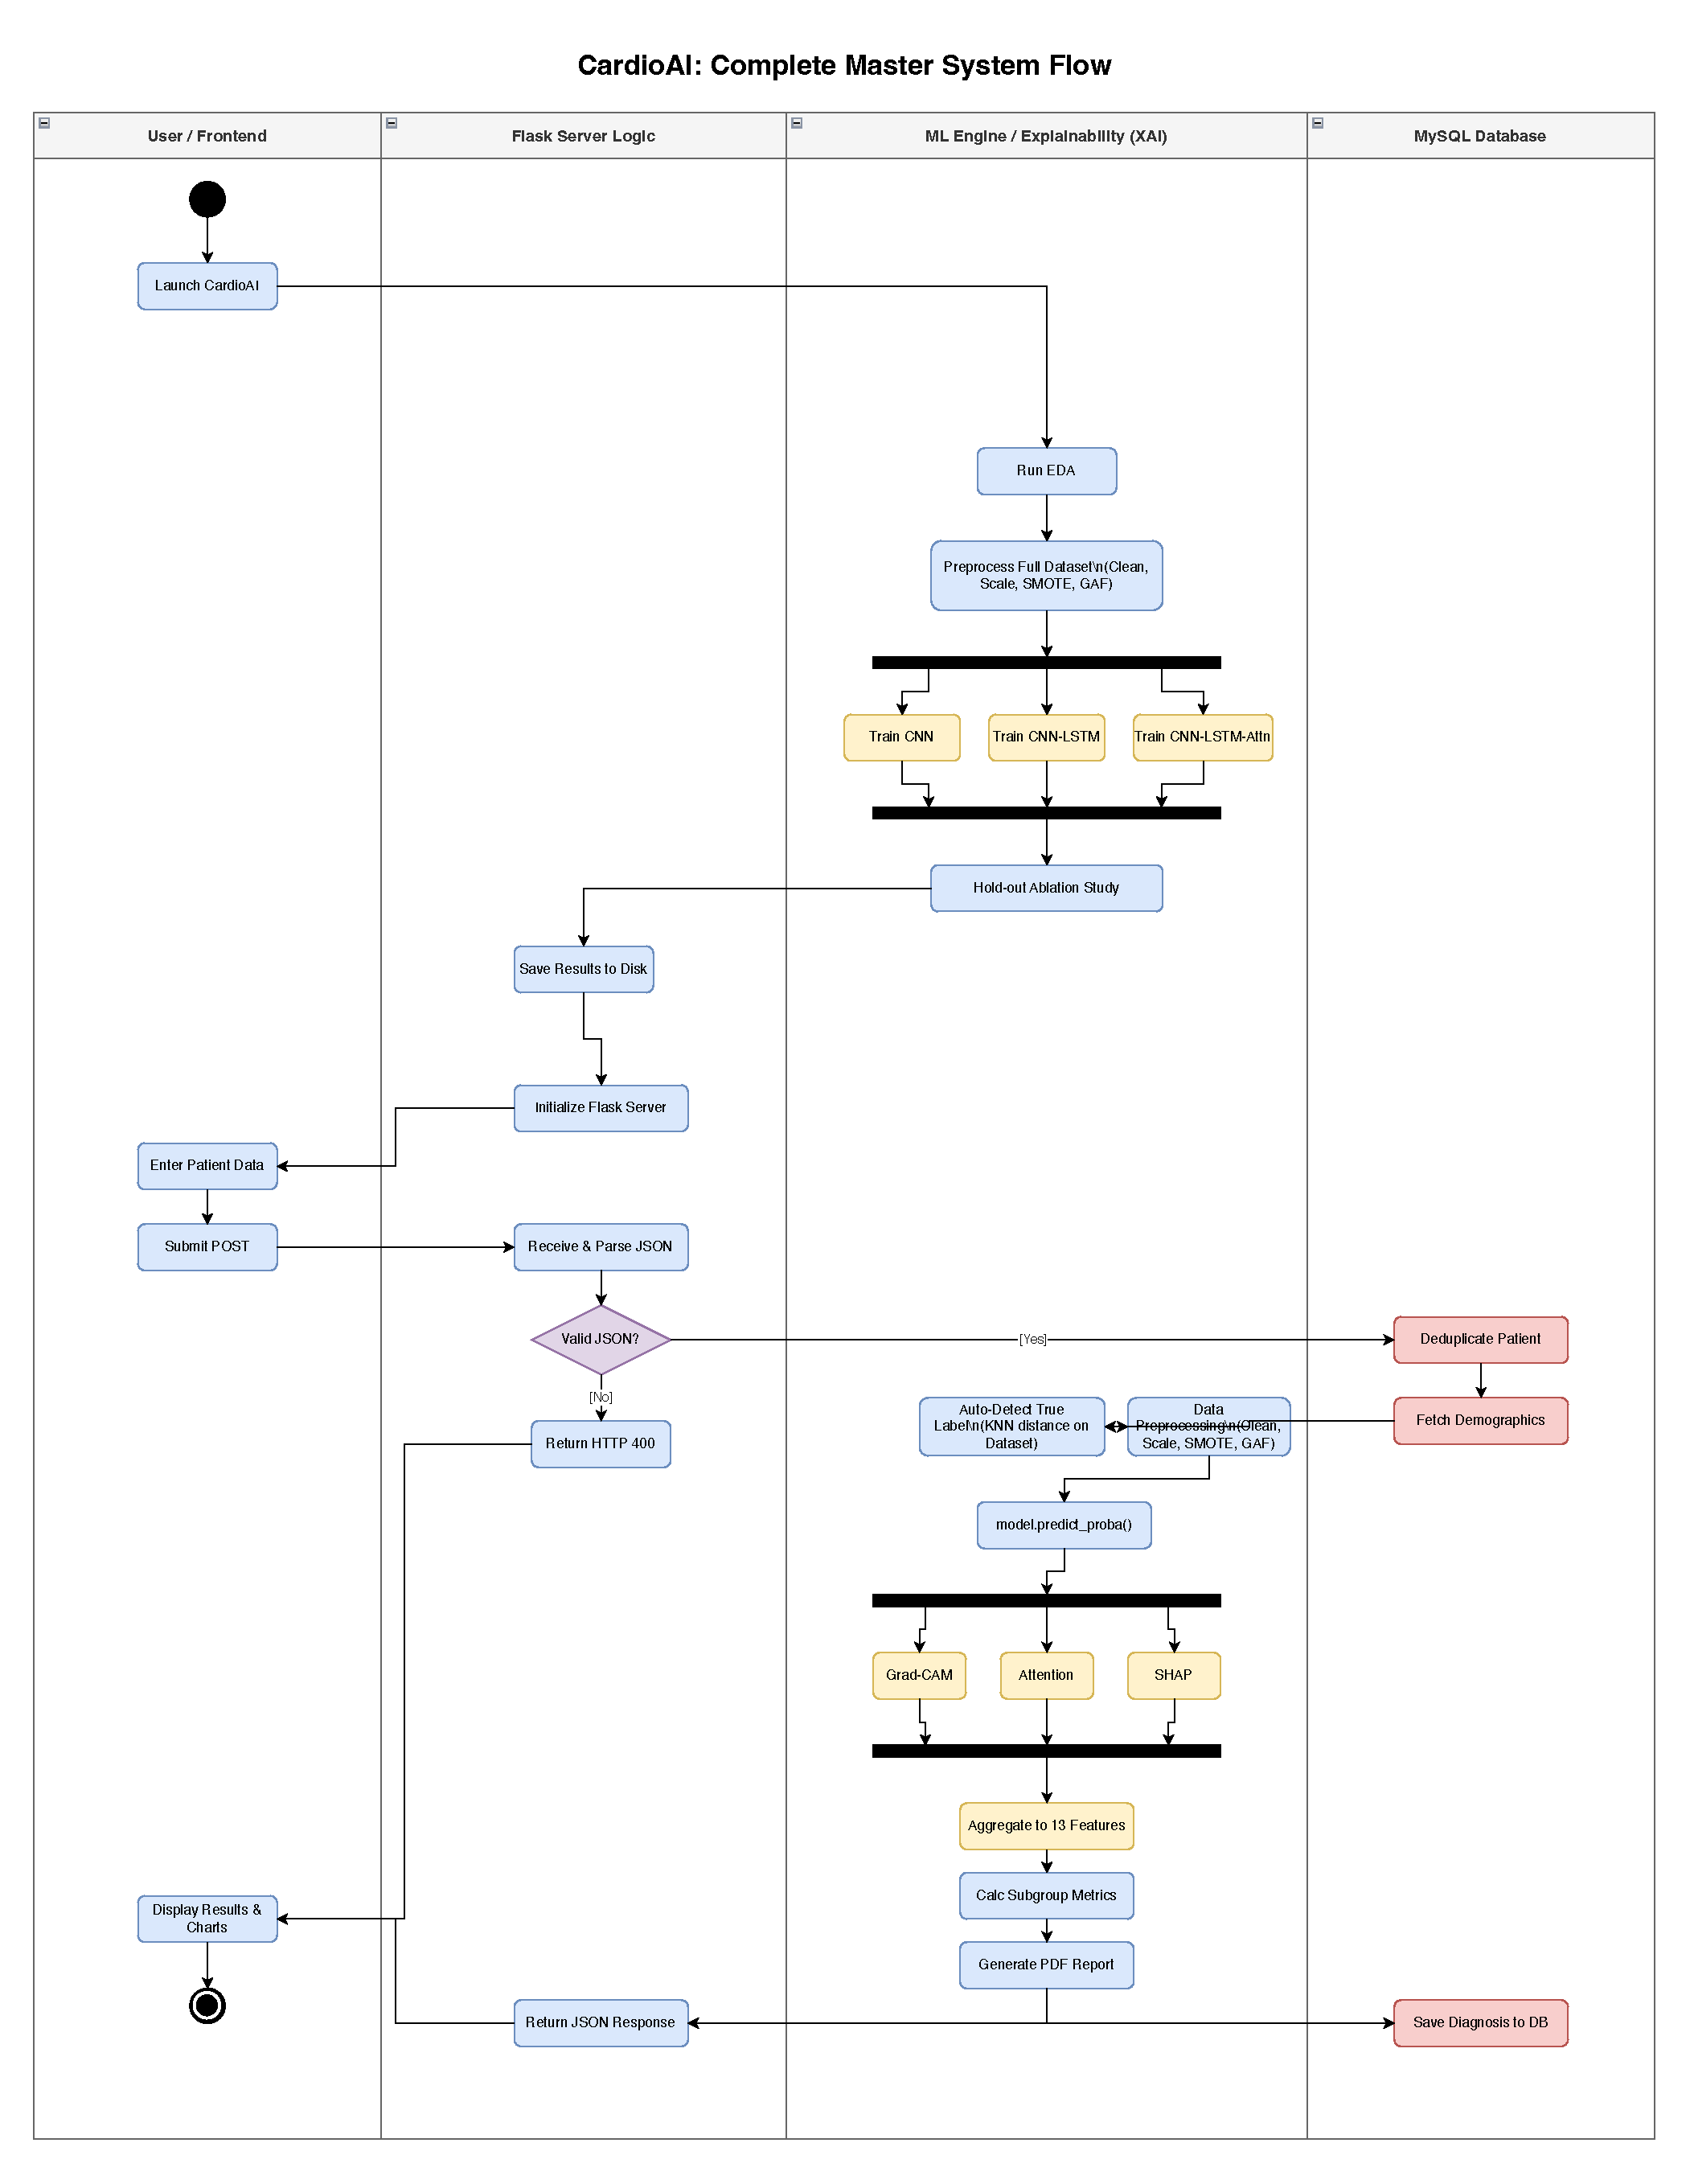
\includegraphics[width=\textwidth,height=0.82\textheight,keepaspectratio]{diagrams/activity diagram Swimlanes.pdf}
    \caption{UML Activity Diagram mapped across specific actor swimlanes (Frontend, Middleware, Backend, DB).}
    \label{fig:activity_swimlanes}
\end{figure}

\clearpage
\subsection{UML Sequence Diagram}
\begin{figure}[H]
    \centering
    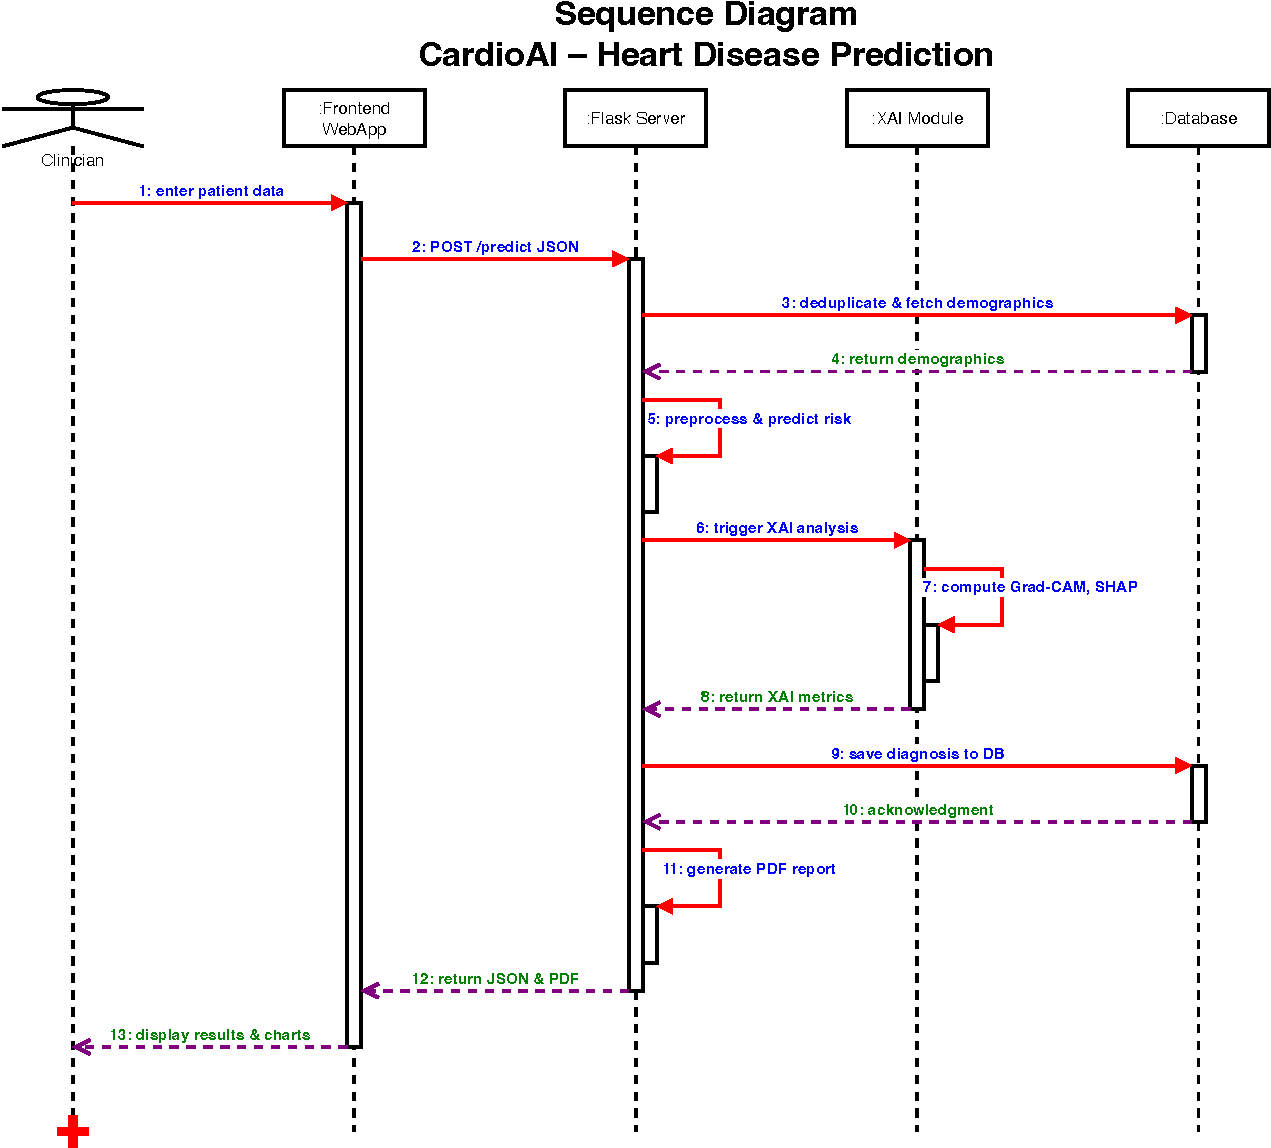
\includegraphics[width=\textwidth,height=0.34\textheight,keepaspectratio]{diagrams/sequence diagram.pdf}
    \caption{UML Sequence Diagram depicting the chronological interaction between system components.}
    \label{fig:sequence}
\end{figure}

\vspace{-0.5em}
\subsection{UML Collaboration Diagram}
\begin{figure}[H]
    \centering
    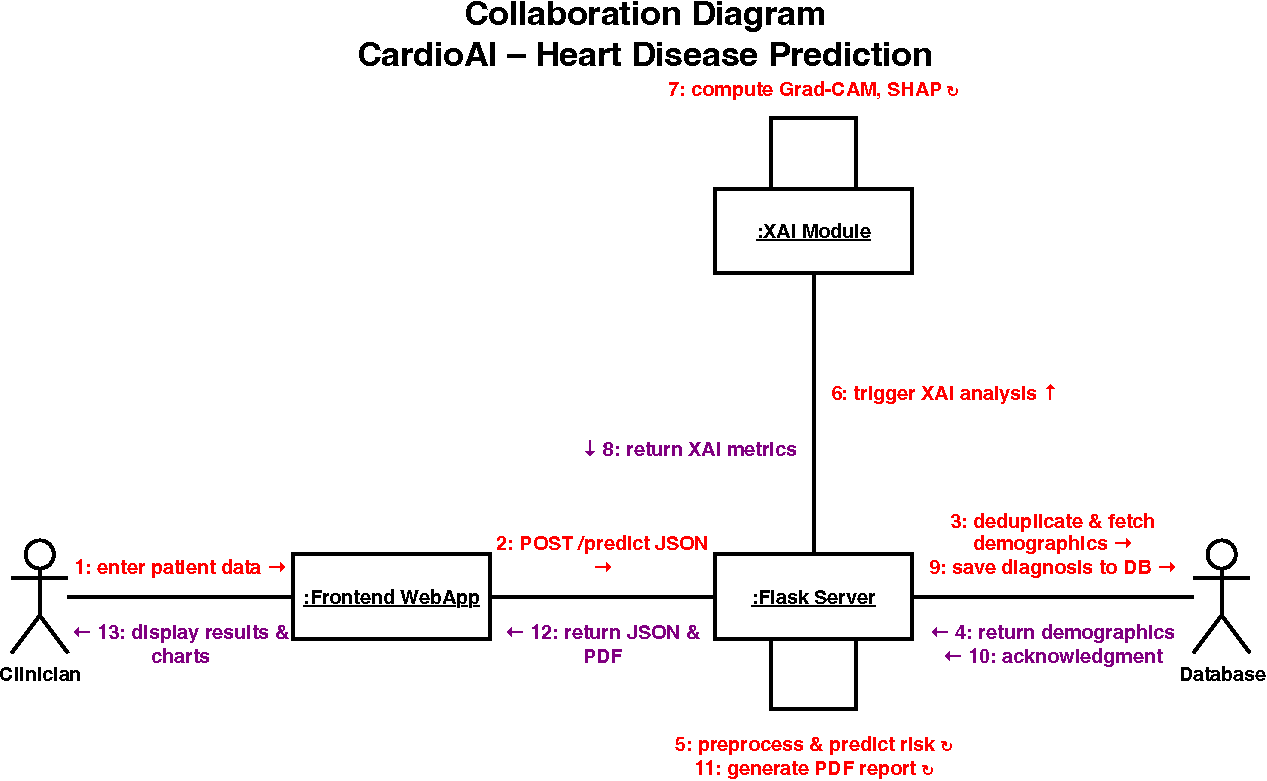
\includegraphics[width=\textwidth,height=0.28\textheight,keepaspectratio]{diagrams/collaboration diagram.pdf}
    \caption{UML Collaboration Diagram highlighting the structural communication links between components.}
    \label{fig:collaboration}
\end{figure}

\clearpage
\subsection{UML Class Diagram}
\begin{figure}[H]
    \centering
    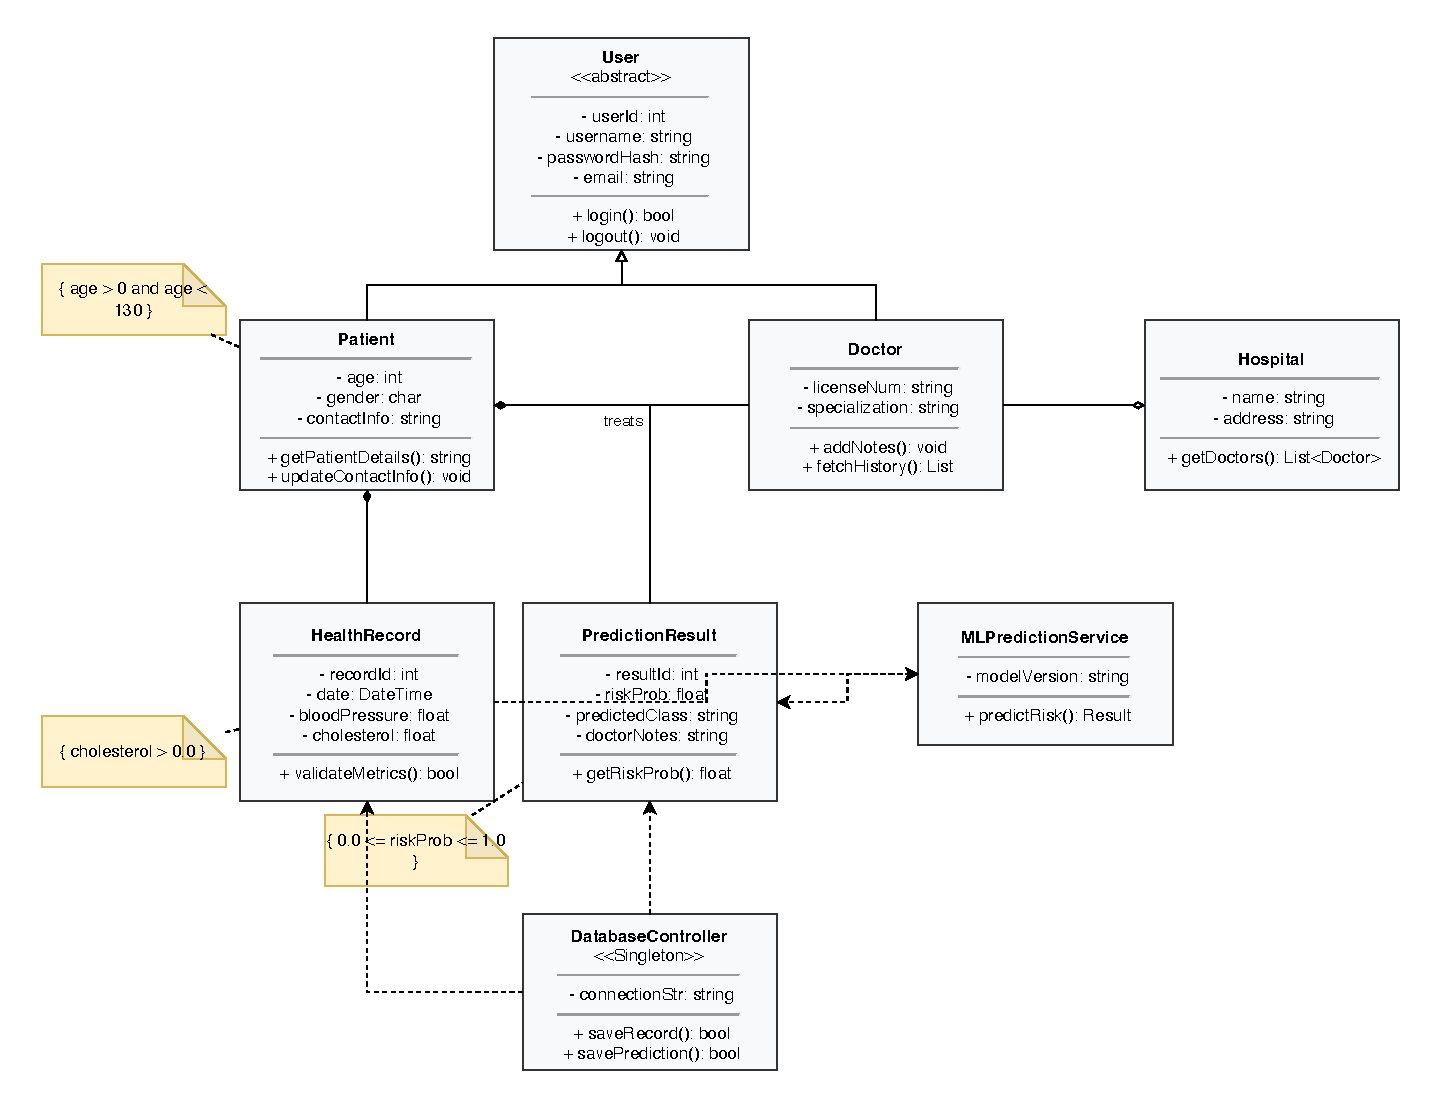
\includegraphics[width=\textwidth,height=0.36\textheight,keepaspectratio]{diagrams/class diagram.pdf}
    \caption{UML Class Diagram depicting domain entities, structural relationships, and OCL constraints.}
    \label{fig:class_diagram}
\end{figure}

\vspace{-0.5em}
\subsection{UML Component Diagram}
\begin{figure}[H]
    \centering
    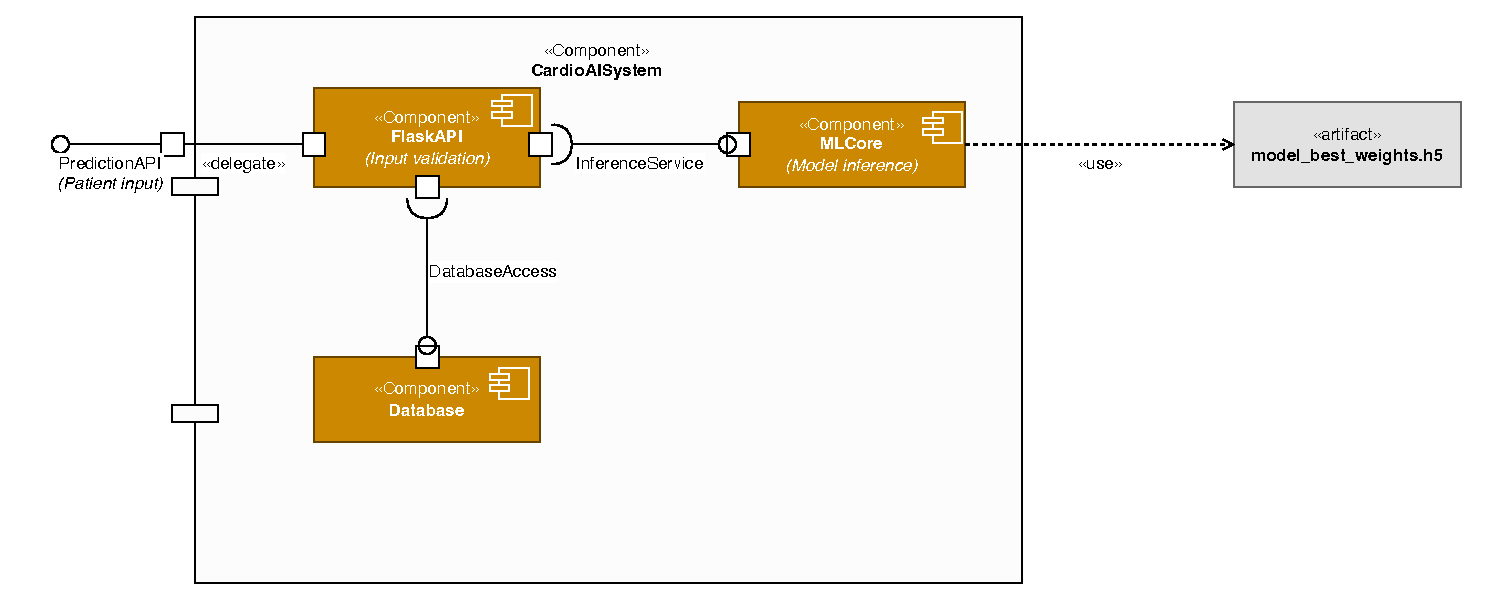
\includegraphics[width=\textwidth,height=0.26\textheight,keepaspectratio]{diagrams/component diagram.pdf}
    \caption{UML Component Diagram defining subsystem boundaries, modular interfaces, and physical dependencies.}
    \label{fig:component_diagram}
\end{figure}

\clearpage
\subsection{Data Flow Diagram (Level 0 - Context Level)}
\begin{figure}[H]
    \centering
    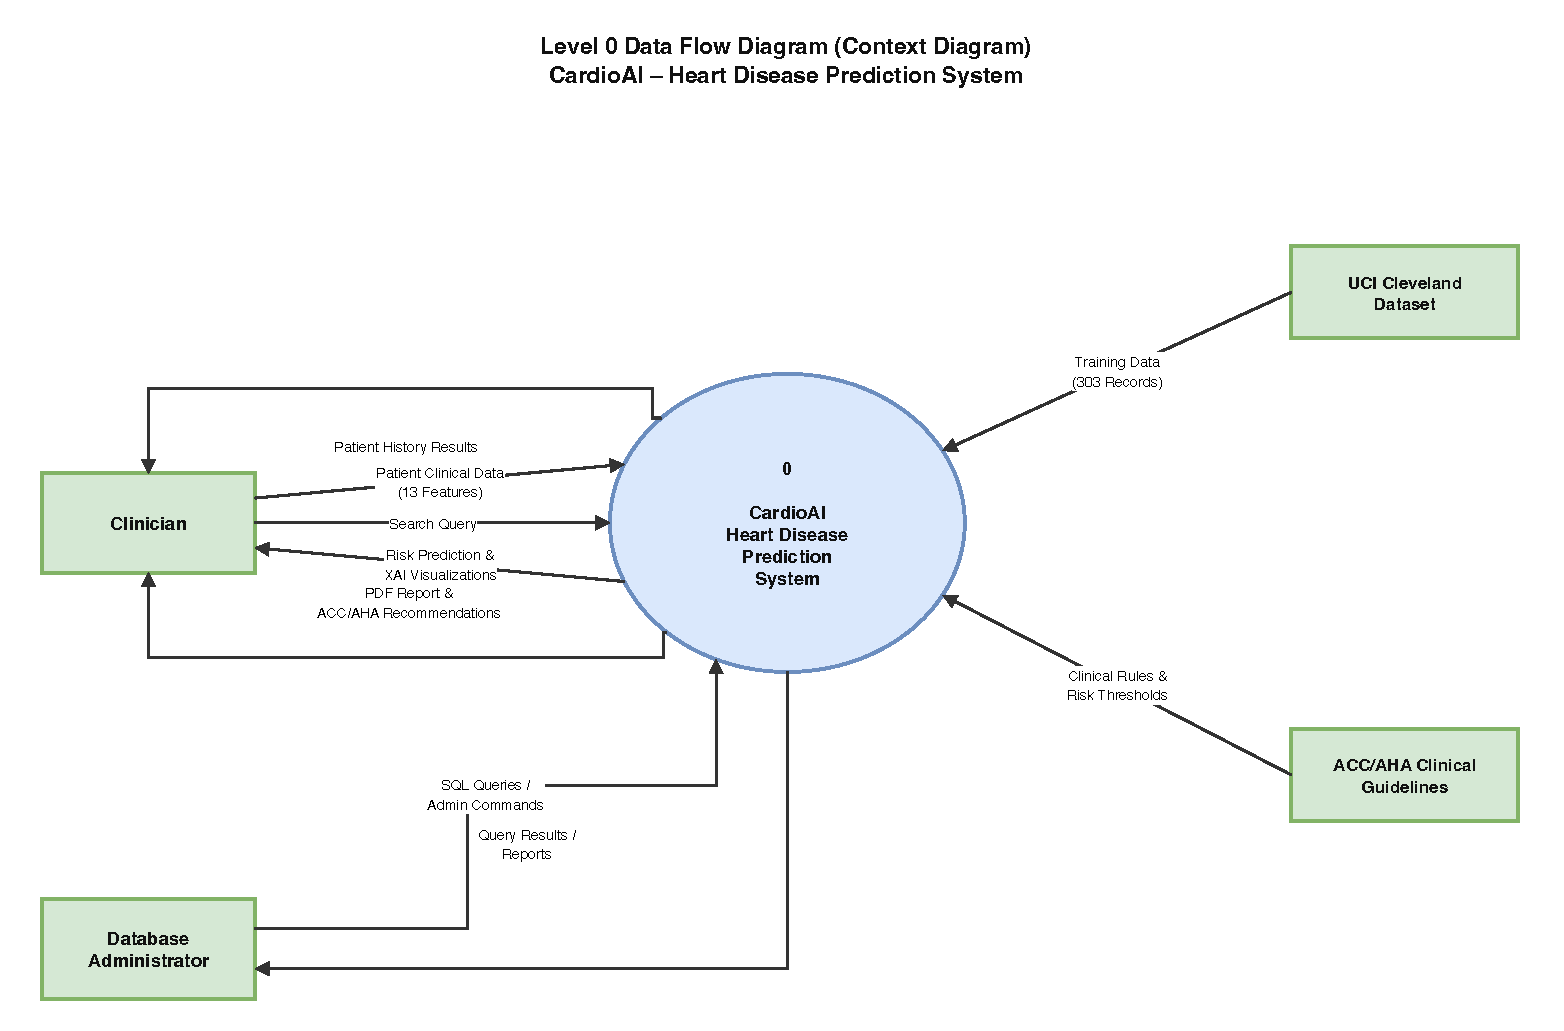
\includegraphics[width=\textwidth,height=0.32\textheight,keepaspectratio]{diagrams/dfd_level_0.pdf}
    \caption{Level 0 Data Flow Diagram (Context Level) illustrating external entities and primary information boundaries.}
    \label{fig:dfd_level_0}
\end{figure}

\vspace{-0.5em}
\subsection{Data Flow Diagram (Level 1 - Functional Decomposition)}
\begin{figure}[H]
    \centering
    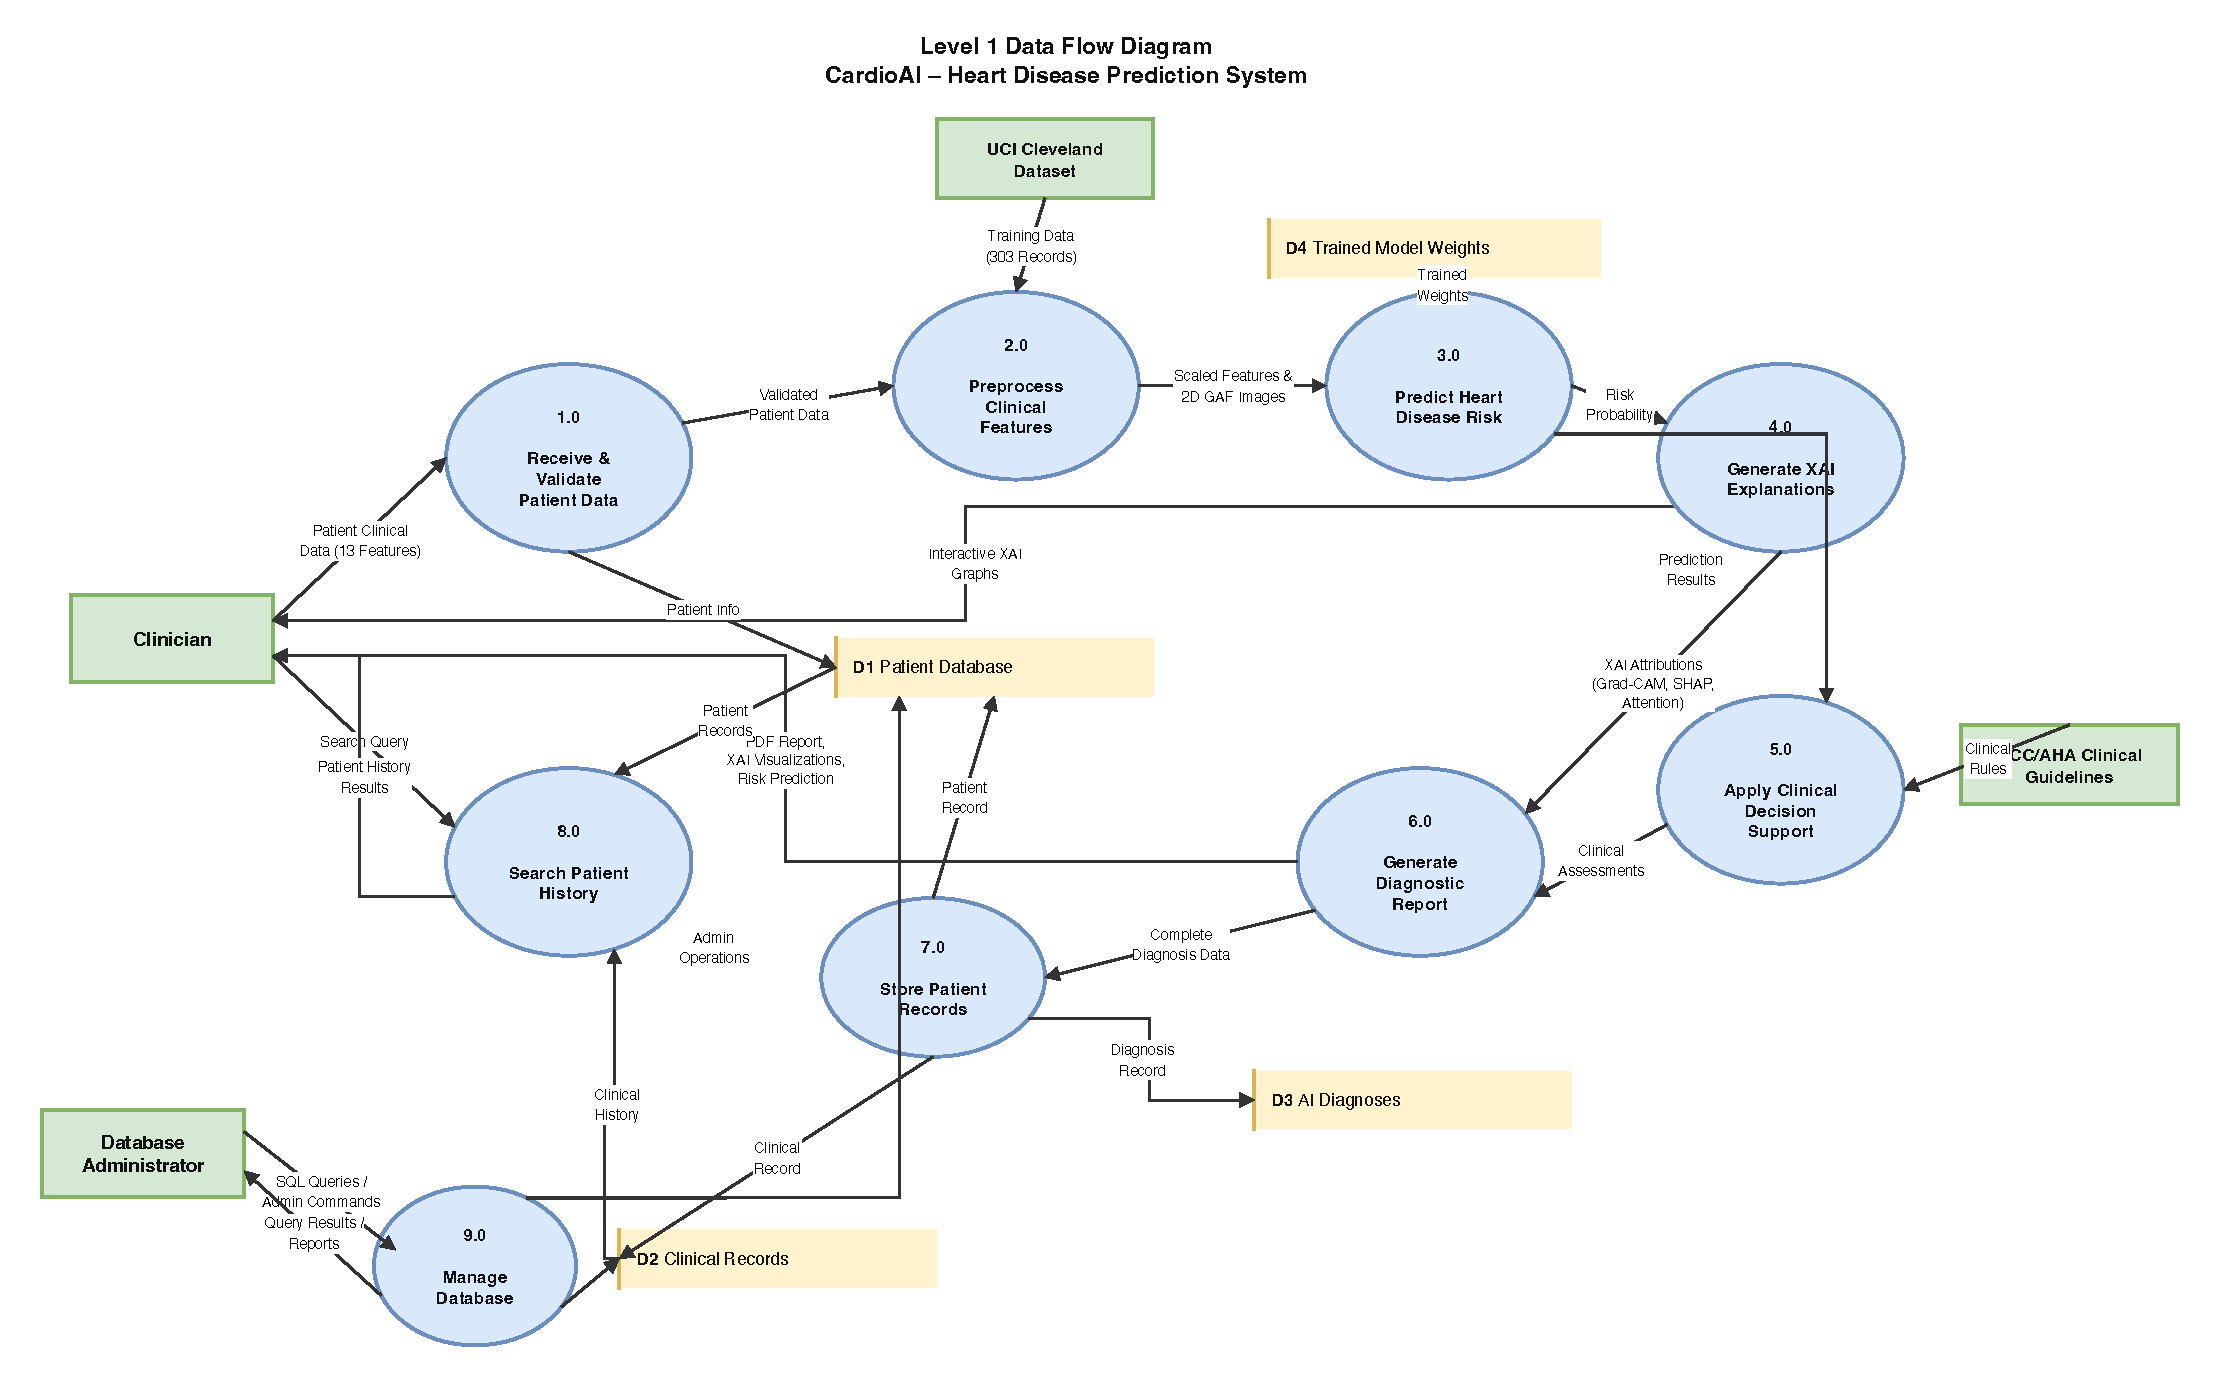
\includegraphics[width=\textwidth,height=0.32\textheight,keepaspectratio]{diagrams/level_1_dfd_Diagram.pdf}
    \caption{Level 1 Data Flow Diagram illustrating modular sub-processes, data stores, and internal information flow.}
    \label{fig:dfd_level_1}
\end{figure}

\clearpage
\subsection{UML Deployment Diagram}
\begin{figure}[H]
    \centering
    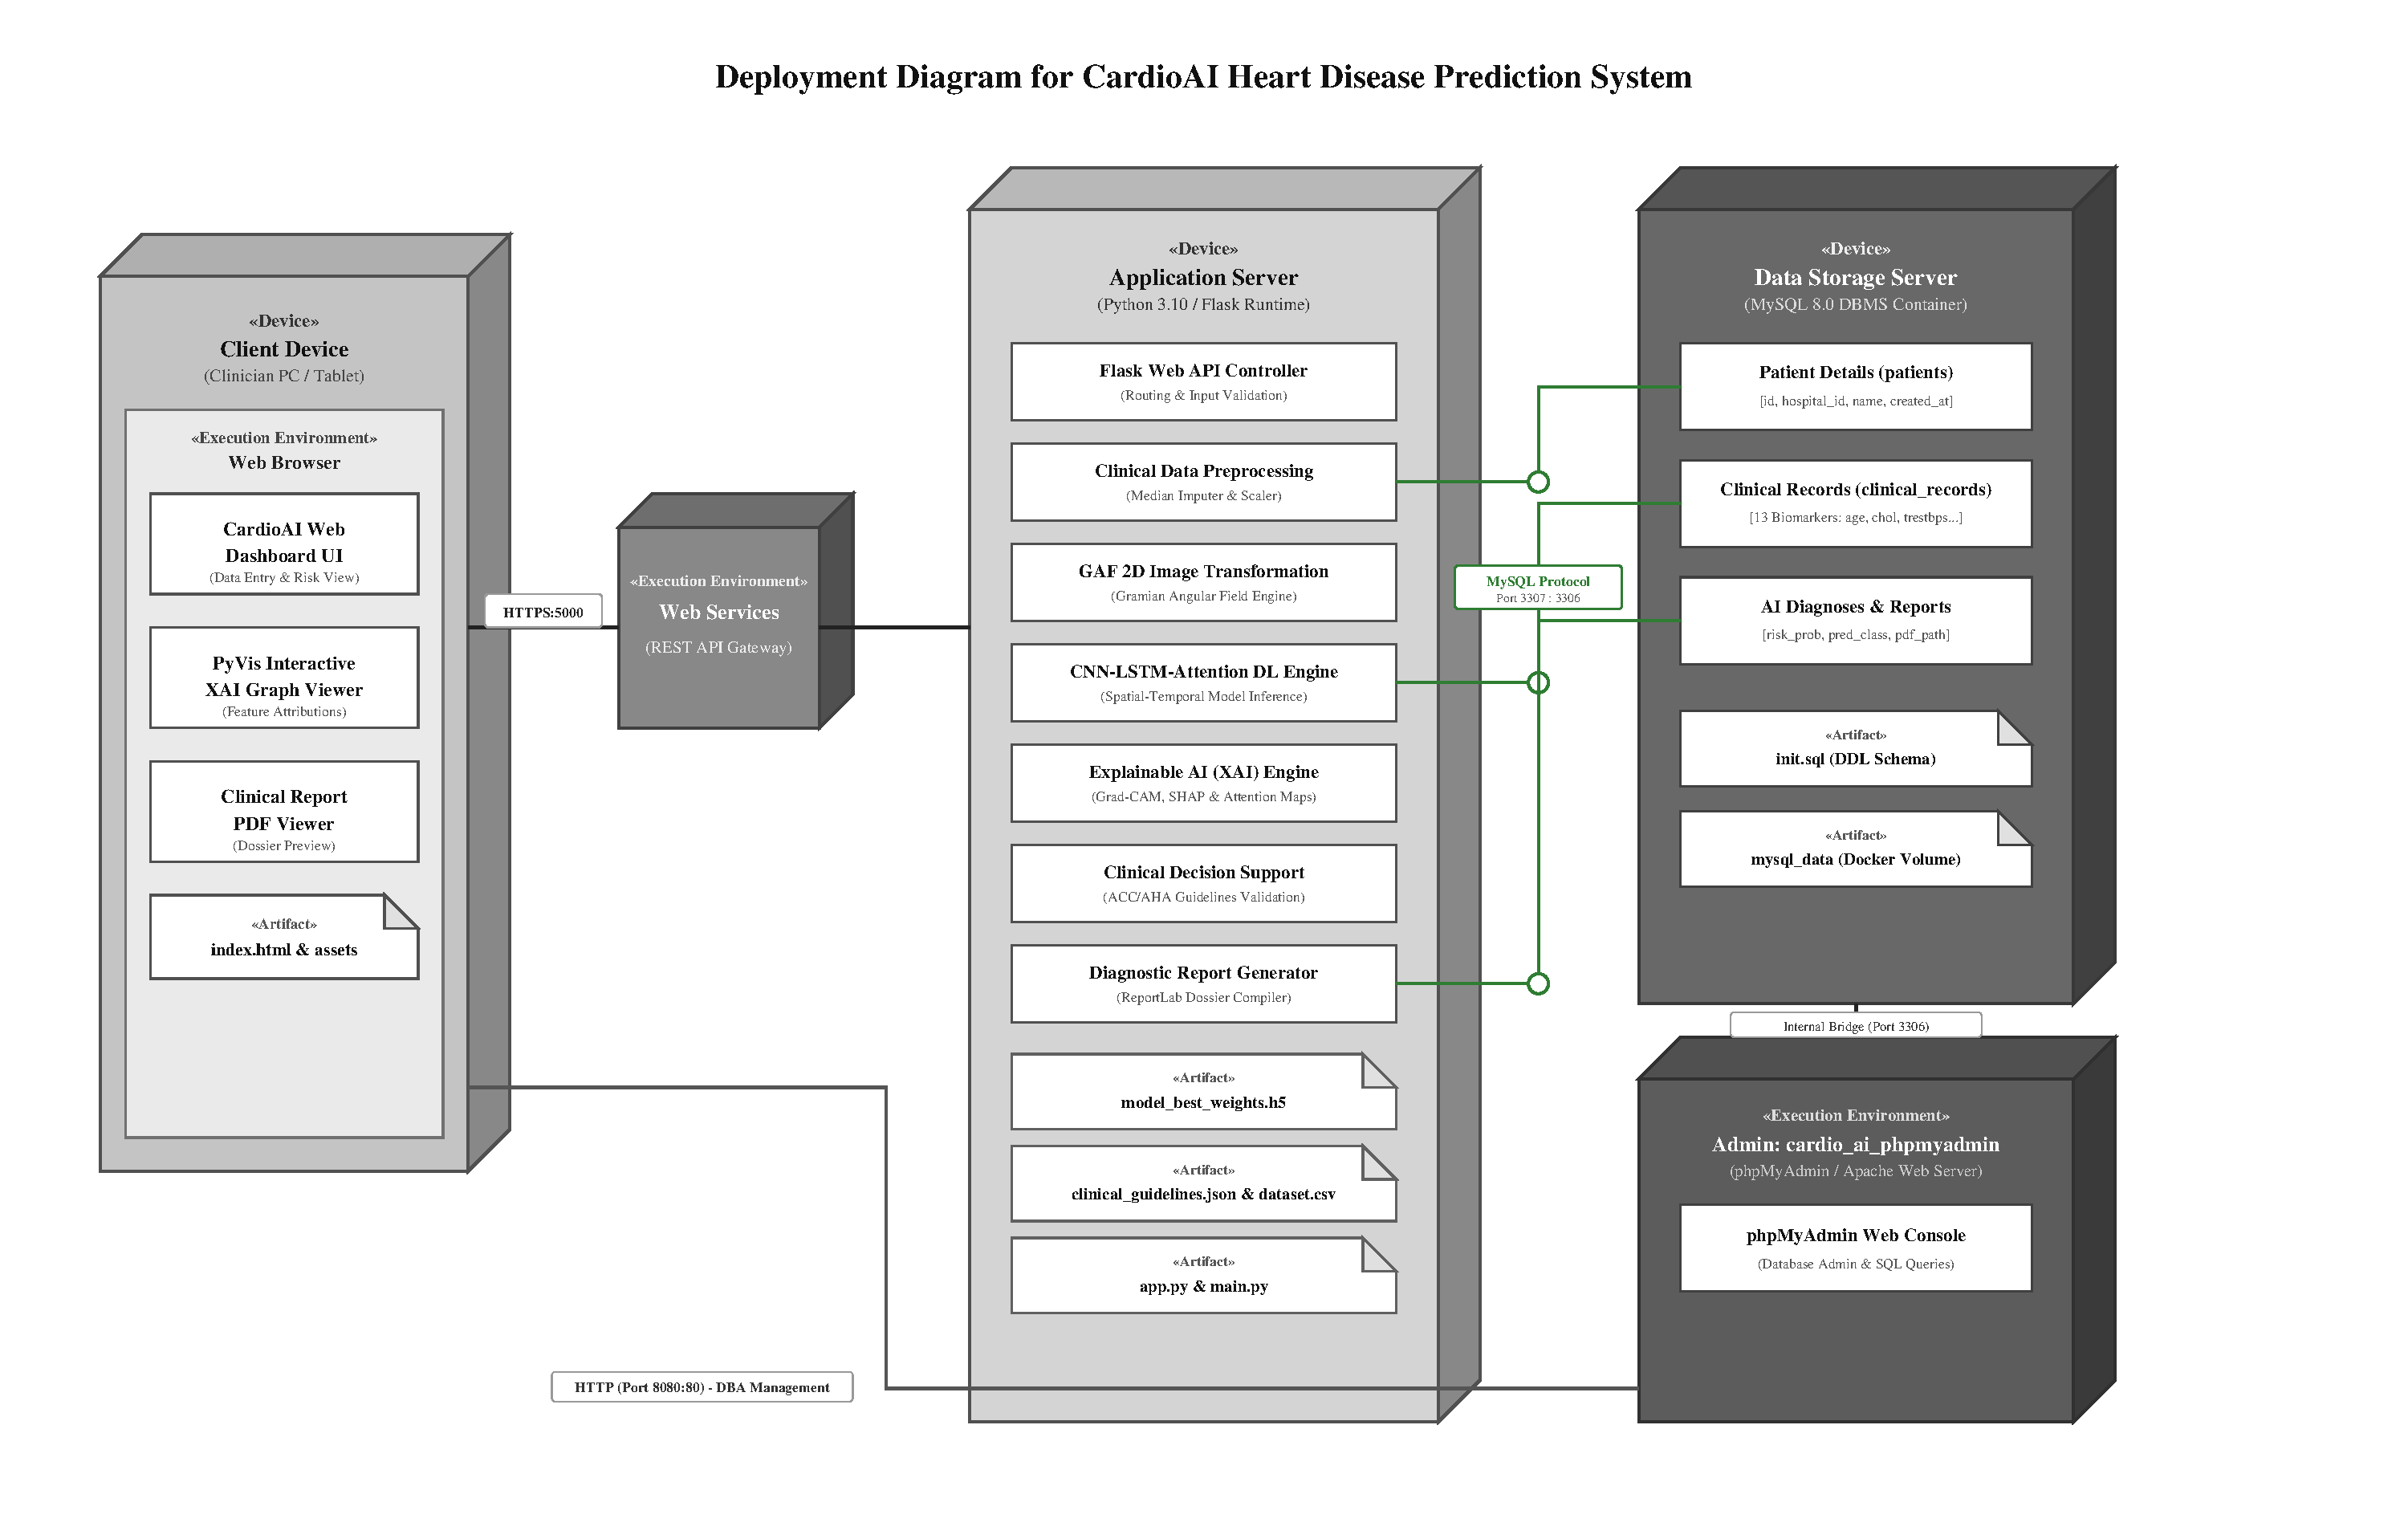
\includegraphics[width=\textwidth,height=0.82\textheight,keepaspectratio]{diagrams/deployment_diagram.pdf}
    \caption{UML Deployment Diagram detailing execution nodes, runtime containers, and communication protocols.}
    \label{fig:deployment_diagram}
\end{figure}


% =========================================================================
% ===== CHAPTER 3: CODING AND IMPLEMENTATION =====
% =========================================================================

\chapter{Coding and Implementation}
\label{chap:coding}

This chapter details the software implementation of Cardio AI across its five core subsystems, structured around a Service-Oriented Architecture (SOA) that decouples frontend presentation, preprocessing, deep learning, explainability, clinical rule evaluation, and REST microservices.

\section{Software Architecture and Subsystem Overview}

The production platform comprises five loosely coupled modules: (1) \texttt{src/preprocessing.py} for data cleaning and 2D GASF transformation; (2) \texttt{src/models.py} and \texttt{src/numpy\_model.py} for hybrid CNN-LSTM-Attention neural modeling; (3) \texttt{src/explainability.py} for multi-method XAI consensus; (4) \path{clinical_guidelines.json} for ACC/AHA heuristic evaluation; and (5) \texttt{app.py} for REST API controller orchestration, MySQL persistence, and ReportLab PDF reporting.

\section{User Interface and Frontend Implementation}

The clinical frontend is engineered as a high-reliability Single Page Application (SPA) featuring a dark cybernetic glassmorphic aesthetic:
\begin{itemize}
    \setlength{\itemsep}{1pt}\setlength{\parskip}{0pt}
    \item \textbf{Glassmorphic Visual Hierarchy:} Dark surfaces (\texttt{\#050811}) with CSS backdrop filters and interactive 3D Vanta.js network topology modulating color according to patient risk.
    \item \textbf{Synchronized Dual-Binding Inputs:} HTML5 range sliders synchronized with numeric inputs and glowing badges evaluating clinical benchmarks (e.g., Stage 2 Hypertension for values exceeding 140 mmHg).
    \item \textbf{Diagnostic Scan and Audio Synthesis:} Animated radar sweep overlay with SVG cardiac pulse and browser-synthesized acoustic cues using the Web Audio API.
    \item \textbf{Analytics Dashboard and Export:} Interactive Plotly.js charts displaying risk probability gauges, live model metrics, multi-method XAI consensus, 2D Grad-CAM heatmaps, narrative summaries, and PDF export.
\end{itemize}

\clearpage
\begin{figure}[H]
    \centering
    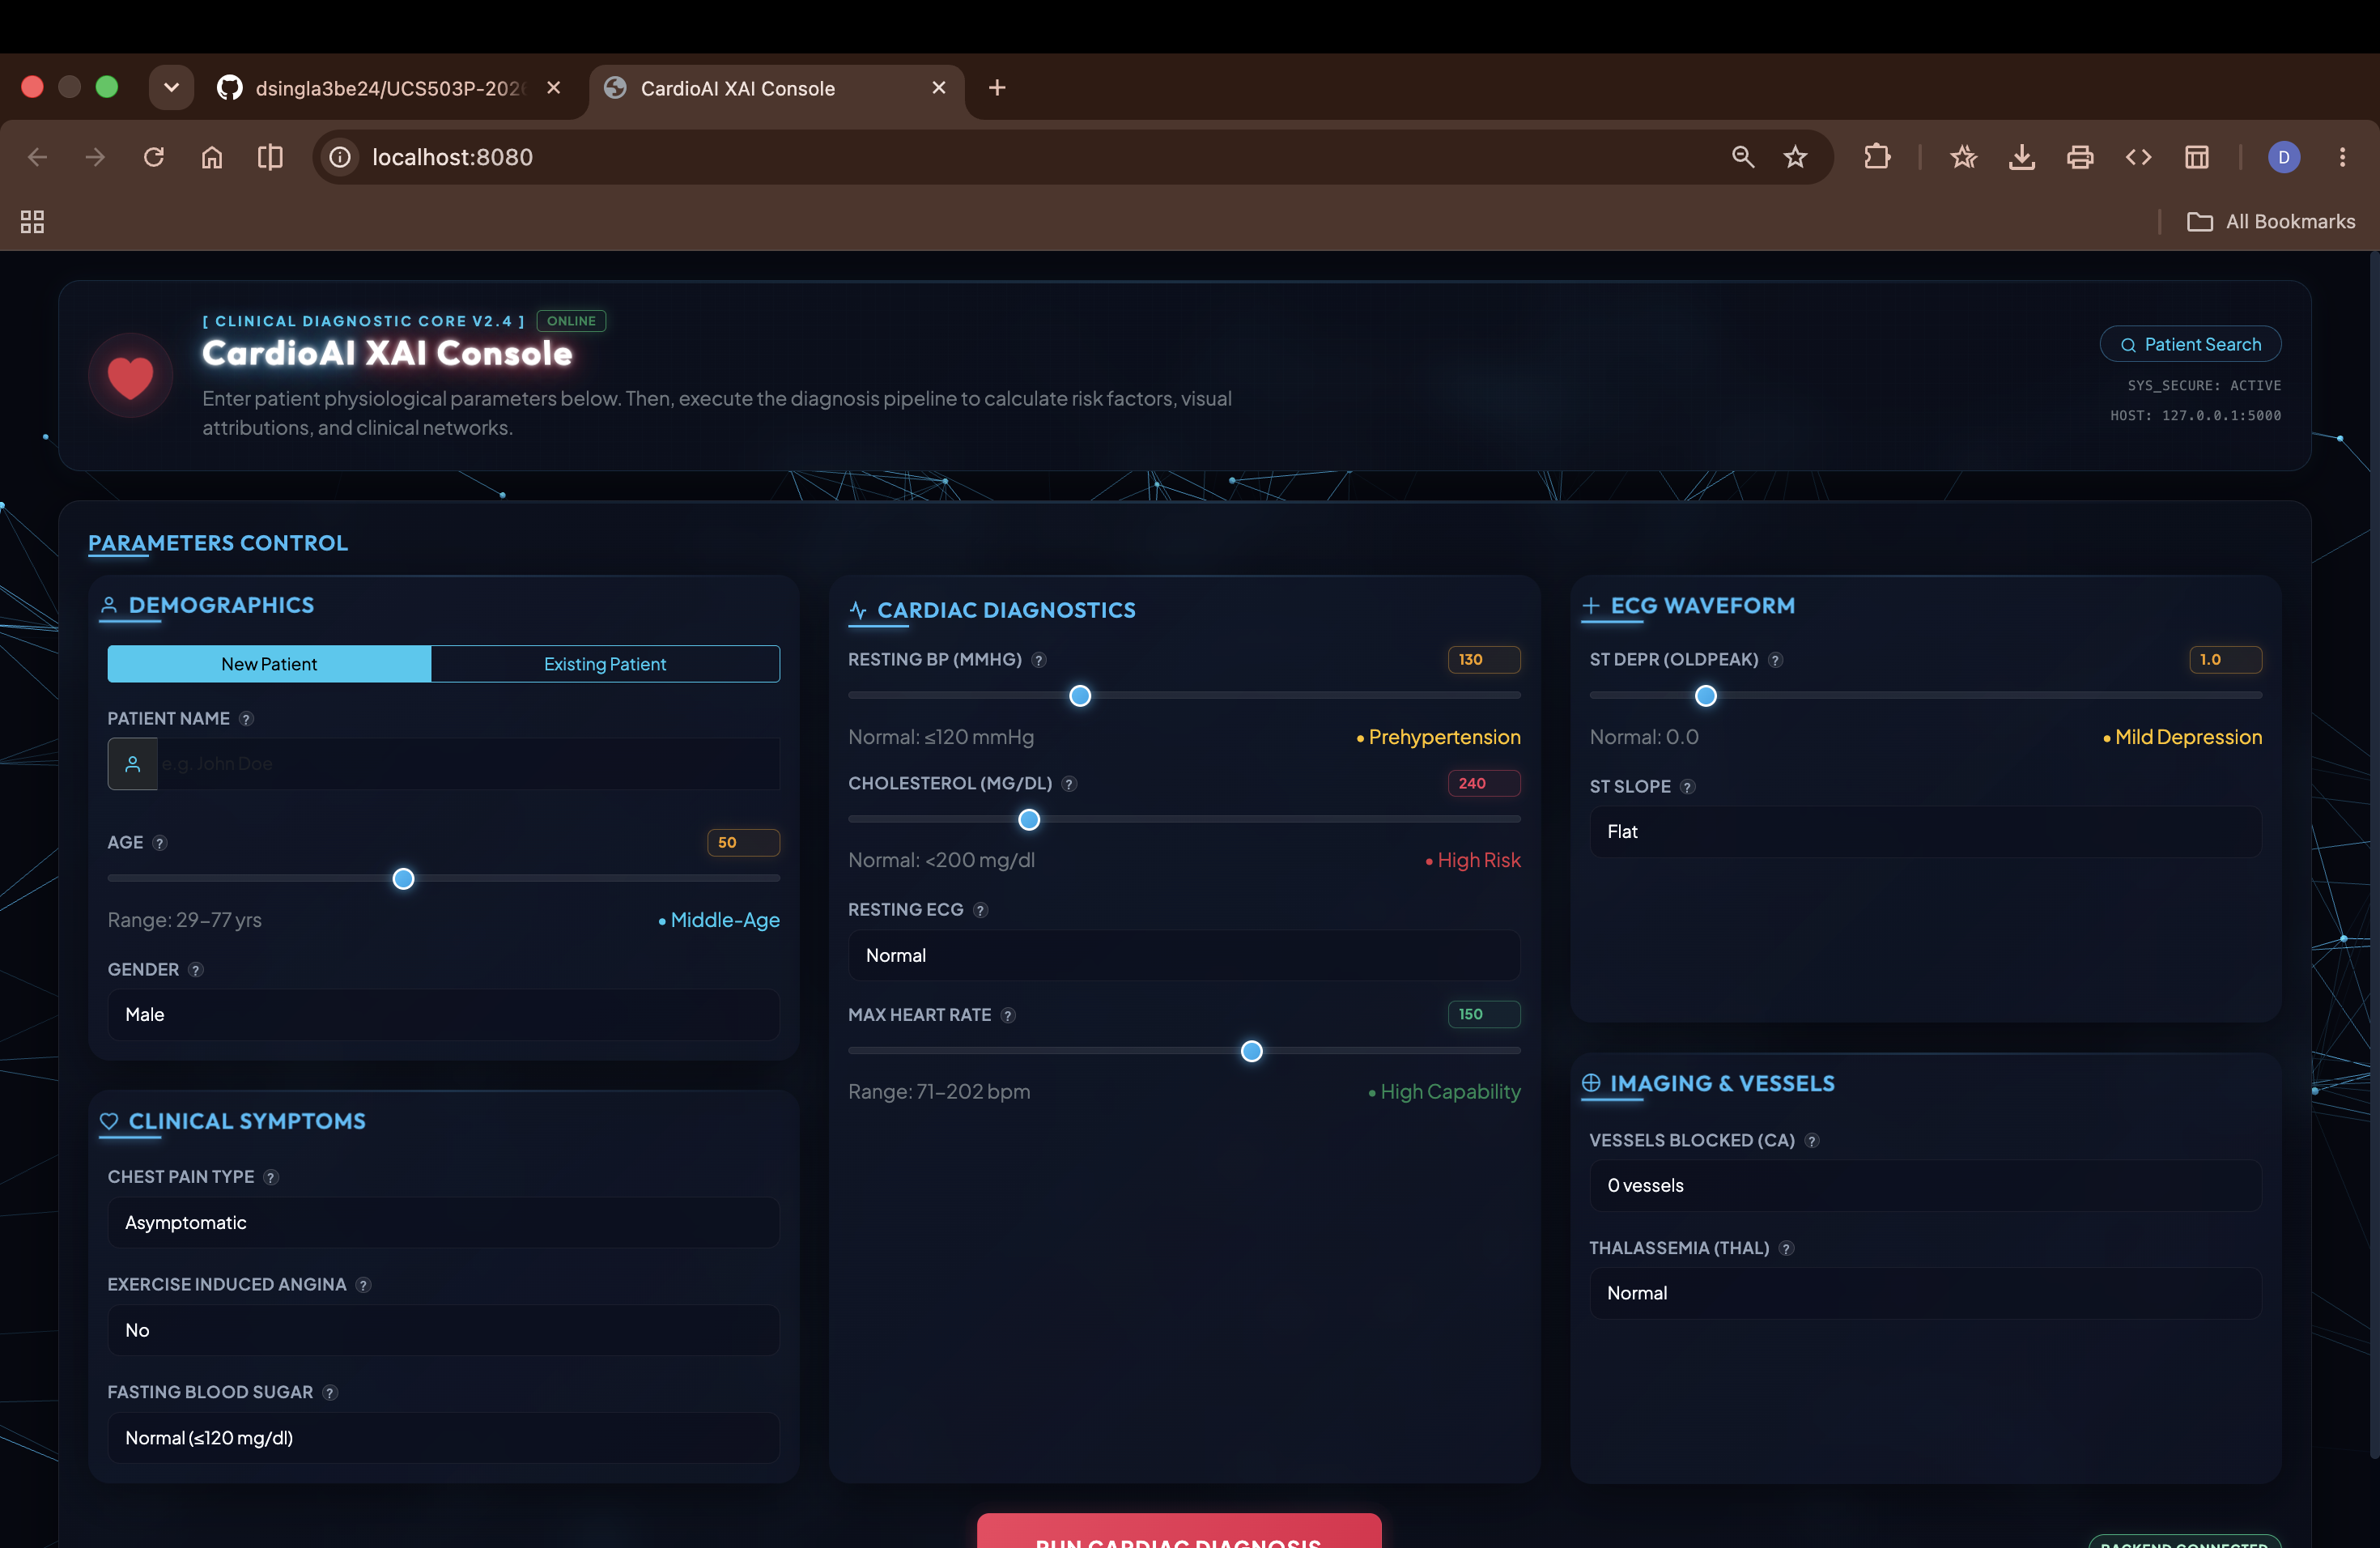
\includegraphics[width=\textwidth,height=0.38\textheight,keepaspectratio]{diagrams/ui_dash_1.png}
    \caption{Initial Data Input Dashboard with 3D Cybernetic Background.}
    \label{fig:ui_dash_1}
\end{figure}

\begin{figure}[H]
    \centering
    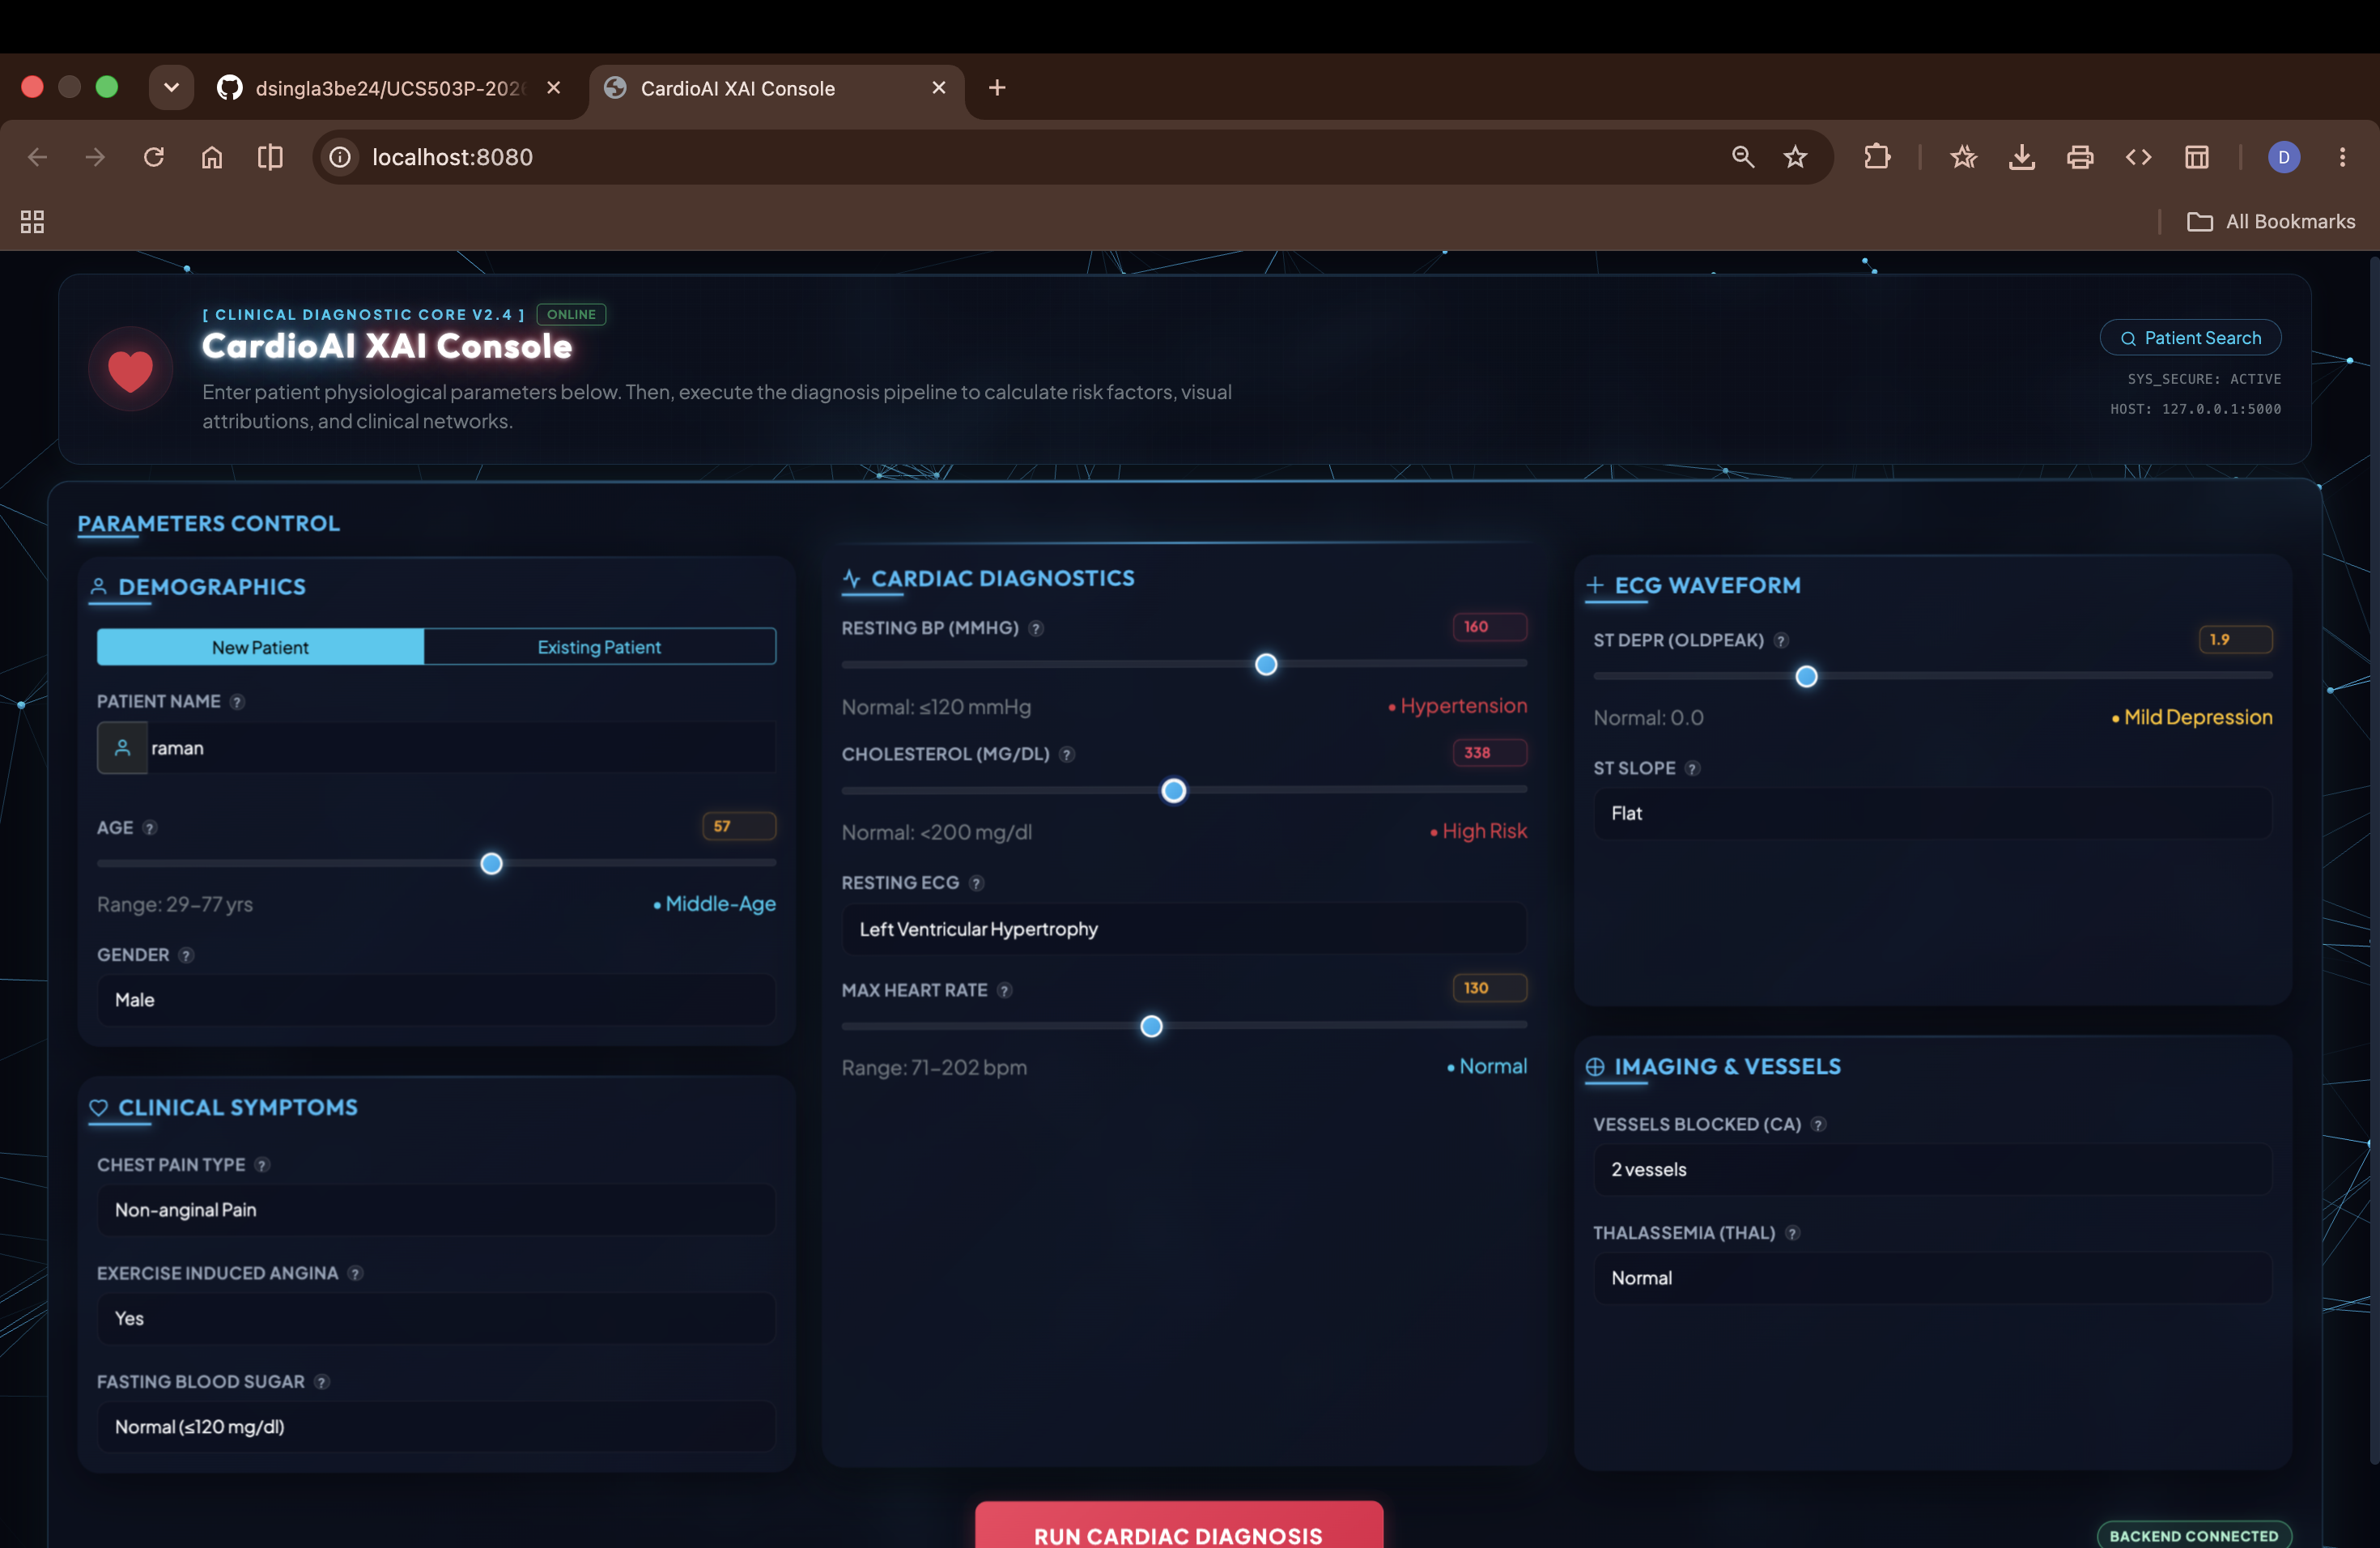
\includegraphics[width=\textwidth,height=0.38\textheight,keepaspectratio]{diagrams/ui_dash_2.png}
    \caption{Active Parameter Entry utilizing synchronized sliders and glowing clinical badges.}
    \label{fig:ui_dash_2}
\end{figure}\clearpage
\begin{figure}[H]
    \centering
    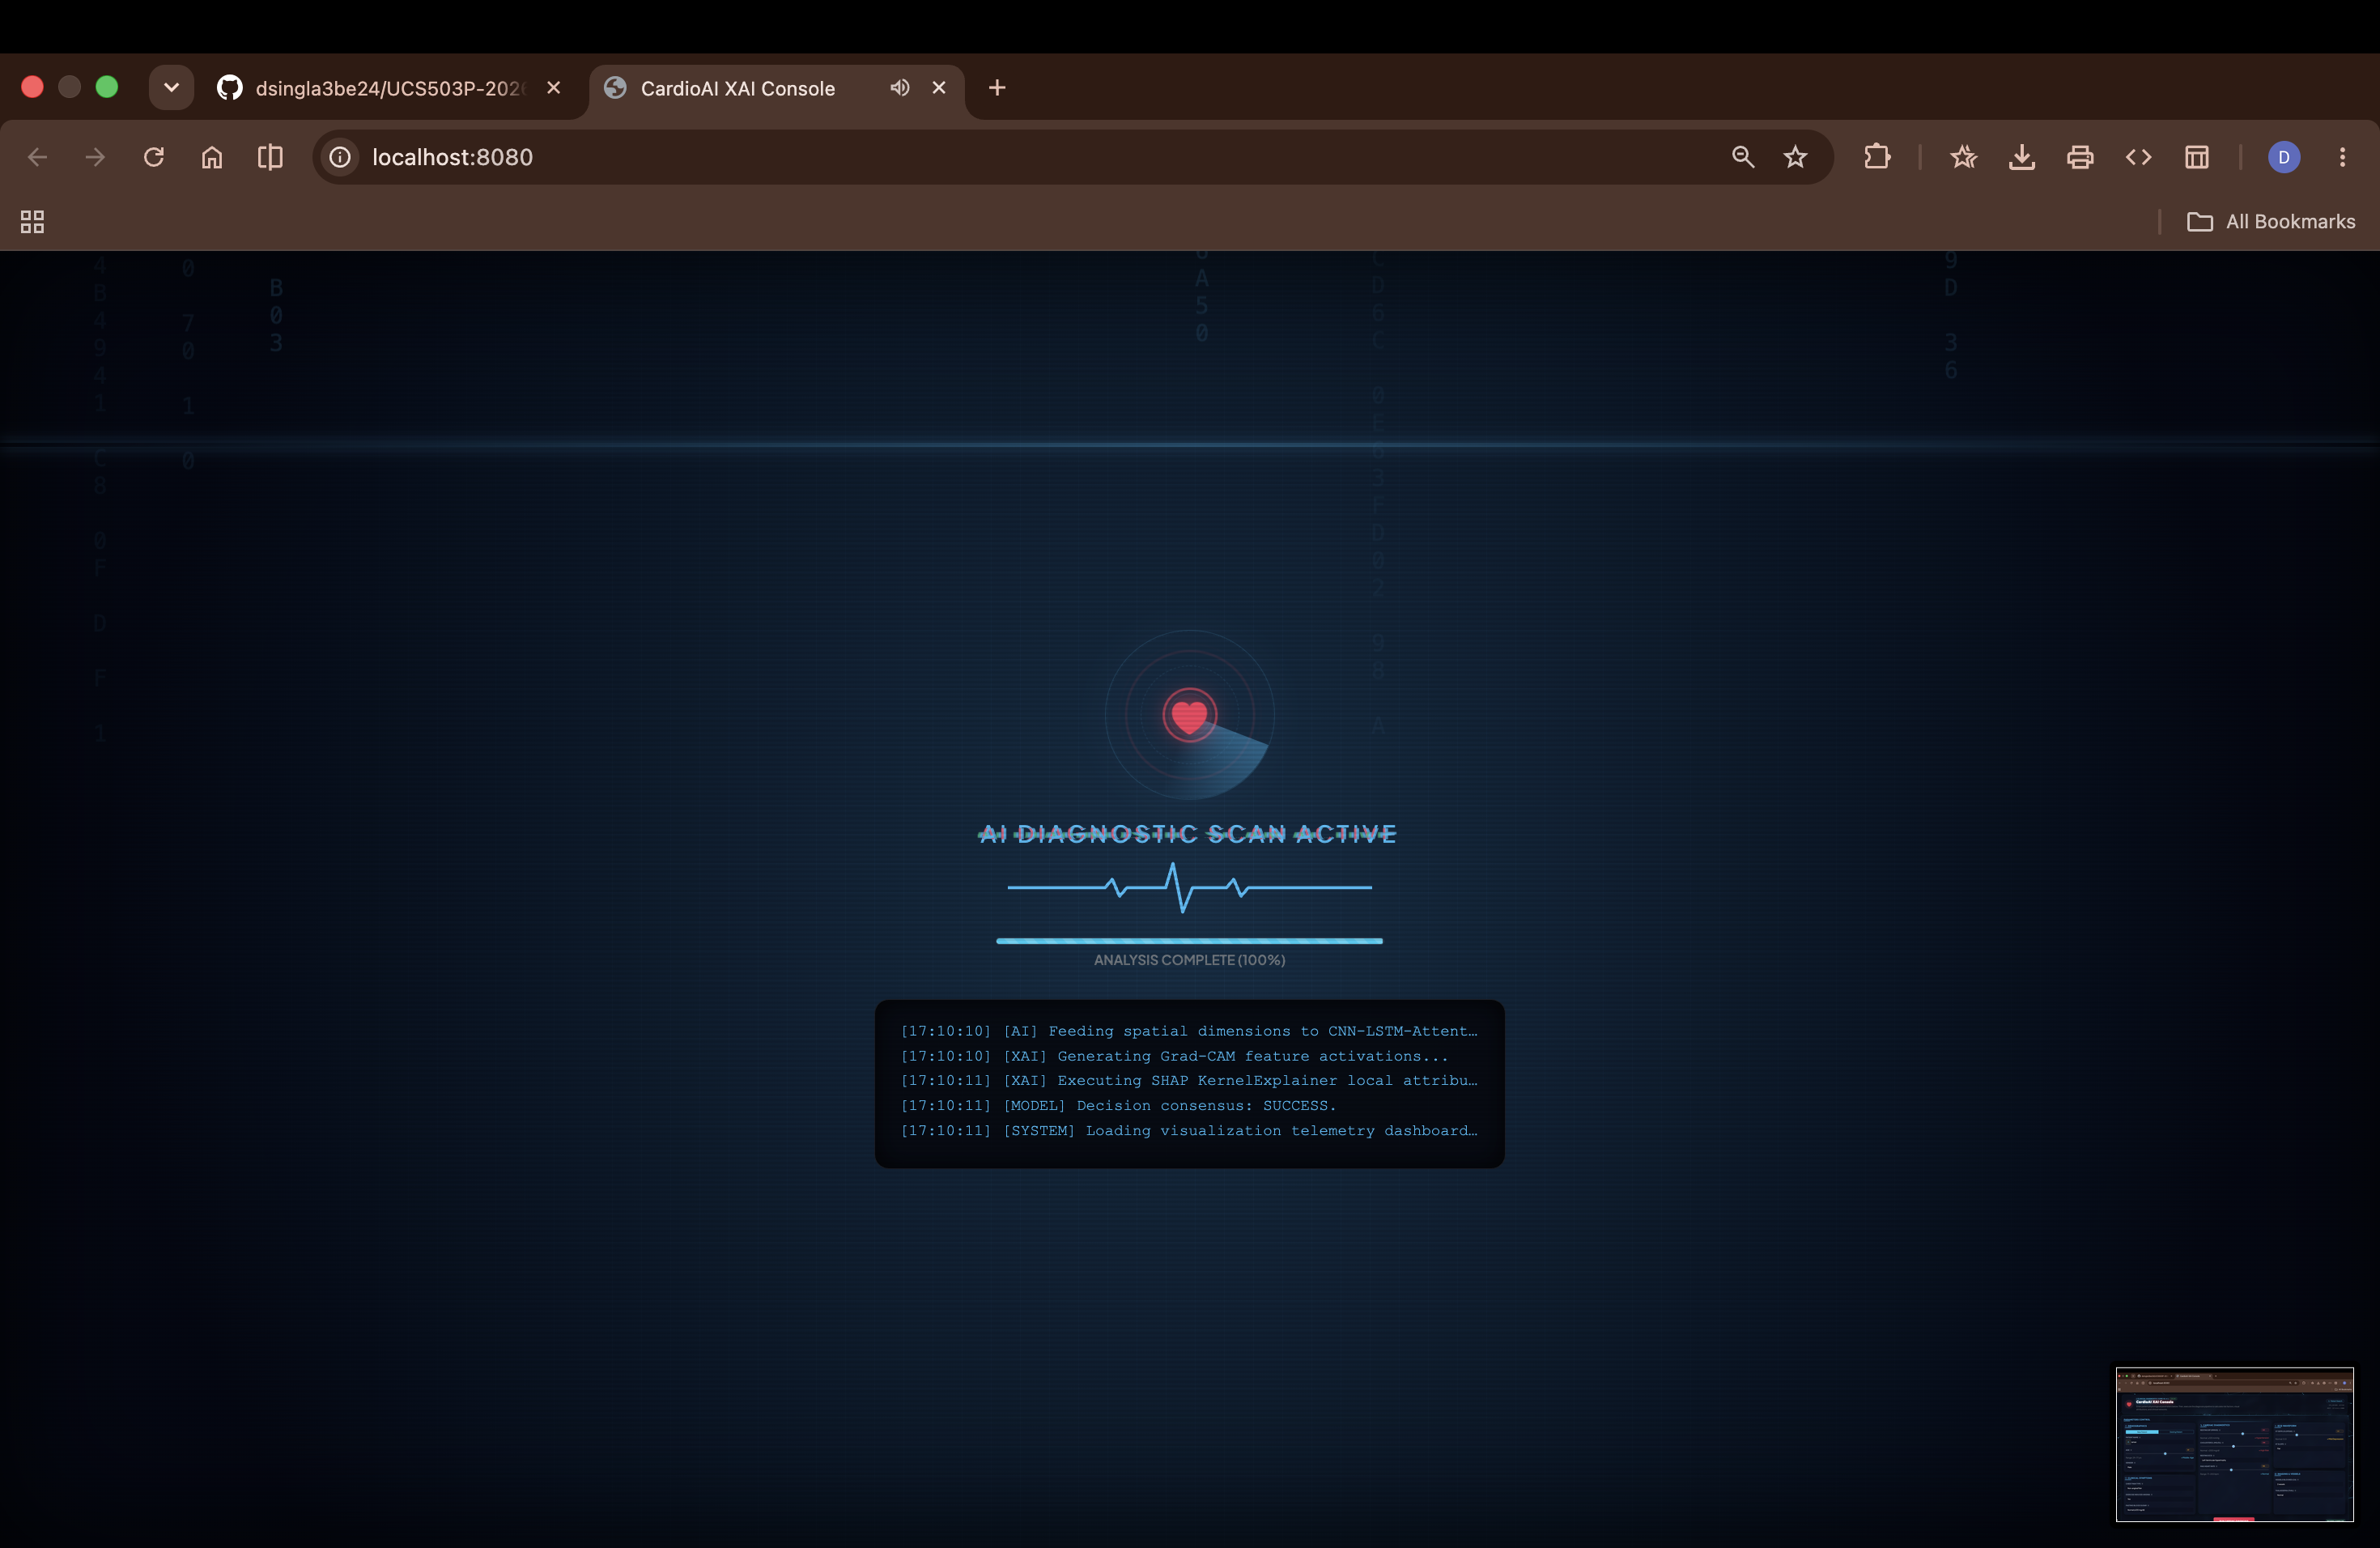
\includegraphics[width=\textwidth,height=0.38\textheight,keepaspectratio]{diagrams/ui_dash_3.png}
    \caption{System Processing State: Radar sweep and diagnostic overlay.}
    \label{fig:ui_dash_3}
\end{figure}

\begin{figure}[H]
    \centering
    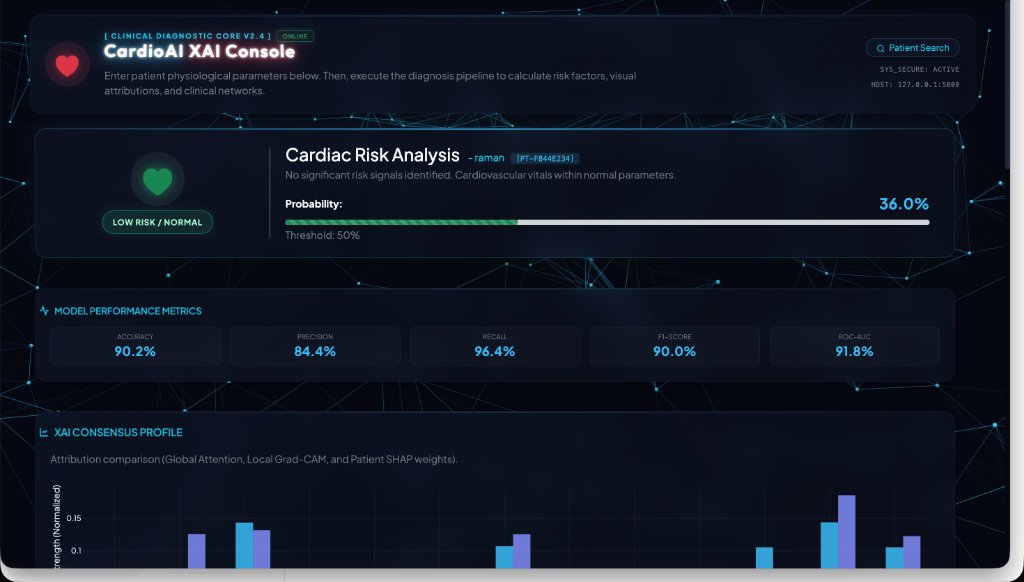
\includegraphics[width=\textwidth,height=0.38\textheight,keepaspectratio]{diagrams/ui_dash_4.png}
    \caption{Results Dashboard: Cardiac Risk Analysis and Real-Time Model Performance Metrics.}
    \label{fig:ui_dash_4}
\end{figure}

\clearpage
\begin{figure}[H]
    \centering
    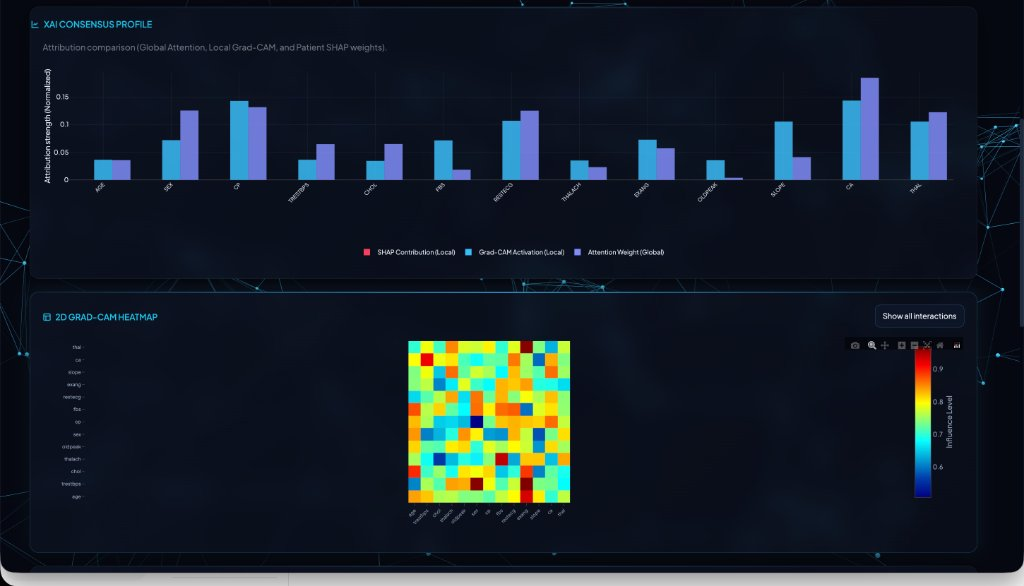
\includegraphics[width=\textwidth,height=0.38\textheight,keepaspectratio]{diagrams/ui_dash_5.png}
    \caption{XAI Consensus Profile: Multi-Method Feature Attributions and 2D Grad-CAM Heatmap.}
    \label{fig:ui_dash_5}
\end{figure}

\begin{figure}[H]
    \centering
    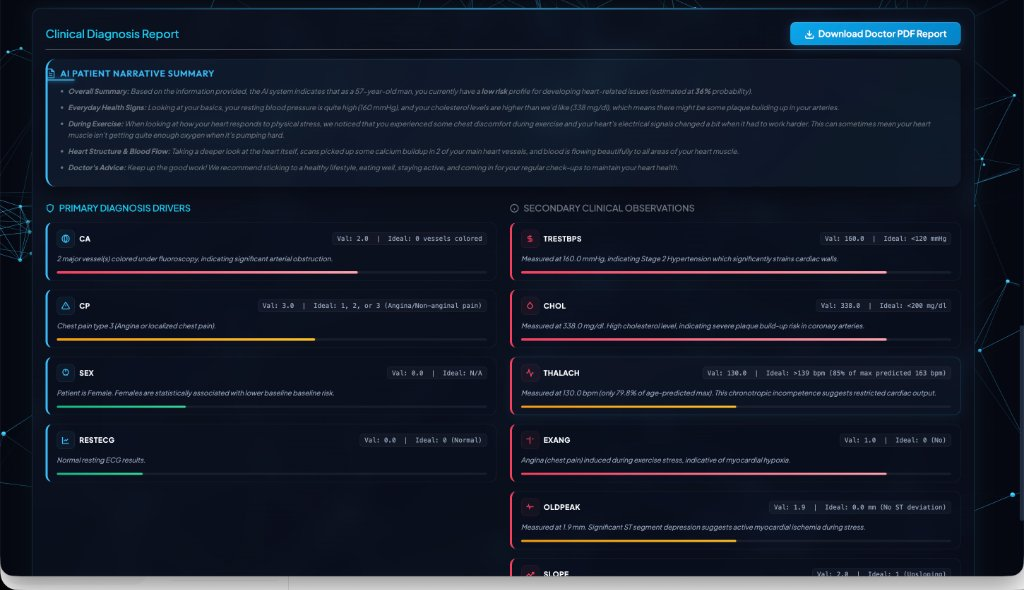
\includegraphics[width=\textwidth,height=0.38\textheight,keepaspectratio]{diagrams/ui_dash_6.png}
    \caption{Clinical Diagnosis Report: AI Patient Narrative Summary, Feature Drivers, and PDF Export.}
    \label{fig:ui_dash_6}
\end{figure}

\clearpage
\section{Module 1: Preprocessing and Vectorized 2D GASF Transformation}

Implemented in \texttt{src/preprocessing.py}, this module ingests raw clinical records, performs median and mode missing-value imputation, rescales numerical vitals to the range between -1 and 1, and projects 1D observations into 28 by 28 Gramian Angular Summation Field tensors. Listing~\ref{lst:gasf} presents this vectorized NumPy implementation:

\begin{lstlisting}[language=Python, caption={Vectorized Gramian Angular Summation Field Transformation (\texttt{src/preprocessing.py})}, label={lst:gasf}]
import numpy as np

def batch_compute_gasf(X):
    N, T = X.shape
    gasf_batch = np.zeros((N, T, T, 1), dtype=np.float32)
    for i in range(N):
        series = X[i]
        min_v, max_v = np.min(series), np.max(series)
        scaled = np.clip(-1.0 + 2.0 * (series - min_v) / (max_v - min_v + 1e-8), -1.0, 1.0)
        phi = np.arccos(scaled)
        cos_phi, sin_phi = scaled, np.sin(phi)
        gasf_batch[i, :, :, 0] = np.outer(cos_phi, cos_phi) - np.outer(sin_phi, sin_phi)
    return gasf_batch
\end{lstlisting}

\section{Module 2: Neural Model Architecture and Attention Mechanism}

Engineered across \texttt{src/models.py} and \texttt{src/numpy\_model.py}, the predictive engine combines 2D convolutional blocks with Batch Normalization and Spatial Dropout, a Bidirectional LSTM recurrent stage for cross-biomarker sequential dependency modeling, and a custom Hierarchical Self-Attention layer. Listing~\ref{lst:attention} defines the attention mechanism, and Listing~\ref{lst:model_builder} outlines network construction in Keras.

\begin{lstlisting}[language=Python, caption={Hierarchical Self-Attention Layer (\texttt{src/numpy\_model.py})}, label={lst:attention}]
import numpy as np

class AttentionLayer:
    def __init__(self, hidden_size, name='tabular_attention'):
        self.name = name
        limit = np.sqrt(6.0 / (2.0 * hidden_size))
        self.W = np.random.uniform(-limit, limit, (hidden_size, hidden_size))
        self.b = np.zeros(hidden_size)
        self.u_query = np.random.uniform(-limit, limit, (hidden_size, 1))
        self.last_attention_weights = None

    def forward(self, h_seq):
        u_t = np.tanh(np.einsum('btd,dk->btk', h_seq, self.W) + self.b)
        scores = np.einsum('btd,dk->btk', u_t, self.u_query)
        exp_scores = np.exp(scores - np.max(scores, axis=1, keepdims=True))
        alphas = exp_scores / np.sum(exp_scores, axis=1, keepdims=True)
        self.last_attention_weights = alphas.copy()
        return np.sum(h_seq * alphas, axis=1), alphas
\end{lstlisting}

\begin{lstlisting}[language=Python, caption={Hybrid Neural Model Construction (\texttt{src/models.py})}, label={lst:model_builder}]
import tensorflow as tf

def build_cnn_lstm_attention(input_shape=(28, 28, 1)):
    inputs = tf.keras.Input(shape=input_shape, name='gasf_input')
    x = tf.keras.layers.Conv2D(32, (3, 3), padding='same', activation='relu')(inputs)
    x = tf.keras.layers.BatchNormalization()(x)
    x = tf.keras.layers.MaxPooling2D((2, 2))(x)
    
    x = tf.keras.layers.Conv2D(64, (3, 3), padding='same', activation='relu')(x)
    x = tf.keras.layers.BatchNormalization()(x)
    x = tf.keras.layers.SpatialDropout2D(0.2)(x)
    x = tf.keras.layers.MaxPooling2D((2, 2))(x)
    
    x = tf.keras.layers.Reshape((7 * 7, 64))(x)
    h_seq = tf.keras.layers.Bidirectional(tf.keras.layers.LSTM(64, return_sequences=True))(x)
    context, alphas = AttentionLayer(hidden_size=128)(h_seq)
    
    x = tf.keras.layers.Dense(32, activation='relu')(context)
    x = tf.keras.layers.Dropout(0.3)(x)
    outputs = tf.keras.layers.Dense(1, activation='sigmoid', name='risk_probability')(x)
    return tf.keras.Model(inputs=inputs, outputs=outputs, name='CardioAI_Engine')
\end{lstlisting}

\section{Module 3: Triple Explainable AI Microservice}

Constructed in \texttt{src/explainability.py}, this module calculates 2D Grad-CAM convolutional activations via TensorFlow GradientTape, estimates Kernel SHAP game-theoretic Shapley values, and extracts intrinsic self-attention weights. Listing~\ref{lst:gradcam} presents the Grad-CAM engine, and Listing~\ref{lst:consensus} details the statistical consensus verification algorithm evaluating Spearman rank correlation and top-4 Jaccard feature overlap.

\begin{lstlisting}[language=Python, caption={Grad-CAM Backpropagation Engine (\texttt{src/explainability.py})}, label={lst:gradcam}]
import tensorflow as tf

def compute_gradcam_2d(model, gasf_img, target_layer_name='conv2d_1'):
    grad_model = tf.keras.models.Model(
        inputs=[model.inputs],
        outputs=[model.get_layer(target_layer_name).output, model.output]
    )
    with tf.GradientTape() as tape:
        conv_outputs, predictions = grad_model(gasf_img)
        loss = predictions[:, 0]
    grads = tape.gradient(loss, conv_outputs)
    pooled_grads = tf.reduce_mean(grads, axis=(0, 1, 2))
    cam_2d = tf.maximum(tf.reduce_sum(conv_outputs[0] * pooled_grads, axis=-1), 0.0)
    cam_1d = tf.reduce_mean(cam_2d, axis=0)
    return (cam_1d / (tf.reduce_max(cam_1d) + 1e-8)).numpy(), (cam_2d / (tf.reduce_max(cam_2d) + 1e-8)).numpy()
\end{lstlisting}

\begin{lstlisting}[language=Python, caption={XAI Consensus and Agreement Metrics (\texttt{src/explainability.py})}, label={lst:consensus}]
from scipy.stats import spearmanr
import numpy as np

def calculate_xai_agreement_metrics(attention_weights, grad_cam_weights, k=4):
    if attention_weights is None or grad_cam_weights is None:
        return {'spearman_corr': 0.0, 'spearman_pvalue': 1.0, 'jaccard_similarity': 0.0}
    corr, pval = spearmanr(attention_weights, grad_cam_weights)
    top_k_att = set(np.argsort(attention_weights)[::-1][:k])
    top_k_gc  = set(np.argsort(grad_cam_weights)[::-1][:k])
    intersection = len(top_k_att.intersection(top_k_gc))
    union = len(top_k_att.union(top_k_gc))
    return {'spearman_corr': float(np.nan_to_num(corr)),
            'spearman_pvalue': float(np.nan_to_num(pval)),
            'jaccard_similarity': float(intersection / union if union > 0 else 0.0)}
\end{lstlisting}

\section{Module 4: Evidence-Based Clinical Rule Engine}

Implemented in \texttt{src/explainability.py} and driven by \path{clinical_guidelines.json}, this module correlates top consensus XAI biomarkers with declarative ACC/AHA cardiology thresholds, grounding raw statistical importance scores into actionable diagnostic observations. Listing~\ref{lst:rules} illustrates the rule-matching evaluation logic:

\begin{lstlisting}[language=Python, caption={Clinical Guideline Evaluation and Evidence Matching (\texttt{src/explainability.py})}, label={lst:rules}]
def evaluate_clinical_guidelines(patient_row, top_features, guidelines):
    narrative_findings = []
    for feat in top_features:
        val = patient_row.get(feat, 0.0)
        if feat == 'trestbps' and val >= 140.0:
            narrative_findings.append(f"Systolic blood pressure ({val:.0f} mmHg) exceeds Stage 2 Hypertension (>=140).")
        elif feat == 'oldpeak' and val >= 1.0:
            narrative_findings.append(f"Exercise ST depression ({val:.1f} mm) indicates myocardial ischemia.")
        elif feat == 'chol' and val >= 240.0:
            narrative_findings.append(f"Serum cholesterol ({val:.0f} mg/dL) exceeds hyperlipidemia threshold (>=240).")
        elif feat == 'ca' and val >= 1.0:
            narrative_findings.append(f"Fluoroscopy detected {int(val)} major coronary vessel(s) with calcification.")
    return narrative_findings
\end{lstlisting}

\section{Module 5: REST API Controller and System Integration}

The Flask REST API controller coordinates payload validation, deep learning inference, XAI consensus calculation, transactional MySQL persistence, and ReportLab PDF compilation into a single unified endpoint responding in under 200 ms. Listing~\ref{lst:flask_api} details this core controller implementation:

\begin{lstlisting}[language=Python, caption={Flask REST API Controller Endpoint (\texttt{app.py})}, label={lst:flask_api}]
from flask import Flask, request, jsonify
import uuid, os
from src.pdf_generator import generate_pdf_report
from src.models import get_or_create_patient, insert_patient_record

app = Flask(__name__)

@app.route("/api/predict", methods=["POST"])
def predict():
    payload = request.get_json()
    if not payload:
        return jsonify({"status": "error", "message": "Missing JSON body"}), 400
    session_id = str(uuid.uuid4())[:8]
    patient_name = payload.get('patient_name', f"Patient-{session_id}")
    patient_id = payload.get('patient_id', f"PT-{session_id.upper()}")
    
    db_id, hosp_id, final_name = get_or_create_patient(patient_name, session_id, patient_id)
    risk_prob, xai_bundle = model_wrapper.predict_with_xai(payload)
    pdf_path = generate_pdf_report(payload, risk_prob, xai_bundle, hosp_id, final_name)
    insert_patient_record(db_id, payload, risk_prob, pdf_path)
    
    return jsonify({
        "status": "success",
        "hospital_patient_id": hosp_id,
        "patient_name": final_name,
        "risk_probability": round(float(risk_prob), 4),
        "risk_category": "HIGH" if risk_prob >= 0.5 else "LOW",
        "xai_metrics": xai_bundle.get("agreement_metrics", {}),
        "report_url": f"/download_report/{os.path.basename(pdf_path)}"
    }), 200
\end{lstlisting}


\chapter{Results and Evaluation}
\label{chap:results}

\section{Testing Methodology}

Testing was conducted across four distinct tiers:
\begin{itemize}
    \setlength{\itemsep}{1pt}\setlength{\parskip}{0pt}
    \item \textbf{Unit Testing:} Validation of MinMax feature scaling, 2D GASF dimensions ($28 \times 28$), custom layer shapes, and ACC/AHA heuristic thresholds.
    \item \textbf{Integration Testing:} End-to-end verification of REST endpoints (\path{/api/predict}), inference pipelines, XAI generation, MySQL persistence, and ReportLab PDF compilation.
    \item \textbf{Stratified Cross-Validation:} 5-fold cross-validation on the training set ($N=242$) to assess stability and hyperparameter sensitivity.
    \item \textbf{Holdout Testing:} Evaluation on an untouched holdout test set ($N=61$, 20\% of cohort) with strict class stratification.
\end{itemize}

\section{Software Engineering Test Cases (SE Lab Deliverable)}

To fulfill Software Engineering verification requirements, the formalized test cases from the official test specification document (\path{test_specification.pdf}) are presented below. Each test case is structured on its own dedicated page.

\clearpage
\subsection{Test Case (Doc:TC\_CARDIO\_01)}

\begin{center}
\small
\renewcommand{\arraystretch}{1.15}
\begin{tabularx}{\textwidth}{|p{2.8cm}|X|p{2.8cm}|X|}
\hline
\textbf{Test Case \#:} & TC\_CARDIO\_01 & \textbf{Test Case Name:} & Predict Heart Disease Risk with Valid Clinical Data \\
\hline
\textbf{System:} & Cardio AI -- Explainable Heart Disease Prediction & \textbf{Subsystem:} & Prediction \& XAI Service (POST /api/predict) \\
\hline
\textbf{Designed by:} & Anirudh & \textbf{Design Date:} & 20/11/2026 \\
\hline
\textbf{Executed by:} & Dhruv Singla & \textbf{Execution Date:} & 20/11/2026 \\
\hline
\textbf{Page:} & 1 of 1 & & \\
\hline
\multicolumn{4}{|p{0.96\textwidth}|}{\textbf{Short Description:} \newline Check that the app gives a risk result, an explanation and a PDF report for a patient's details.} \\
\hline
\end{tabularx}
\end{center}

\vspace{-0.4em}
\noindent\textbf{Pre-conditions:}
\begin{enumerate}
    \setlength{\itemsep}{1pt}
    \setlength{\parskip}{0pt}
    \item The app is running at \url{http://localhost:8080}.
    \item The sample patient details (given in step 2) are ready.
\end{enumerate}

\vspace{-0.4em}
\noindent\textbf{Execution Steps:}
\begin{center}
\small
\renewcommand{\arraystretch}{1.10}
\setlength{\tabcolsep}{3pt}\begin{tabularx}{\textwidth}{|>{\centering\arraybackslash}p{0.9cm}|>{\raggedright\arraybackslash}p{3.5cm}|>{\raggedright\arraybackslash}X|>{\centering\arraybackslash}p{1.4cm}|>{\centering\arraybackslash\footnotesize}p{1.7cm}|}
\hline
\textbf{Step} & \textbf{Action} & \textbf{Expected System Response} & \textbf{Status} & \textbf{Comment} \\
\hline
1 & Open \url{http://localhost:8080} in the browser. & The app page opens. & \textbf{PASS} & {\footnotesize Works.} \\
\hline
2 & Enter patient details: Age 63, Male, CP 4, BP 145, Chol 233, FBS 1, RestECG 2, Thalach 150, Exang 0, Oldpeak 2.3, Slope 3, CA 0, Thal 7. Submit. & The details are accepted. & \textbf{PASS} & {\footnotesize Works.} \\
\hline
3 & Check the prediction result. & Shows ``Heart Disease Risks Detected'' (probability $\approx 0.9995$). & \textbf{PASS} & {\footnotesize Correct.} \\
\hline
4 & Check explanation shown with result. & Charts and clinical note are shown. & \textbf{PASS} & {\footnotesize Shown.} \\
\hline
5 & Click the PDF report link. & The PDF report opens. & \textbf{PASS} & {\footnotesize Opens.} \\
\hline
\end{tabularx}
\end{center}

\vspace{-0.4em}
\noindent\textbf{Post-conditions:}
\begin{enumerate}
    \setlength{\itemsep}{1pt}
    \setlength{\parskip}{0pt}
    \item The prediction and explanation are shown.
    \item The PDF report is saved in \texttt{static/temp/}.
\end{enumerate}

\clearpage
\subsection{Test Case (Doc:TC\_CARDIO\_02)}

\begin{center}
\small
\renewcommand{\arraystretch}{1.15}
\begin{tabularx}{\textwidth}{|p{2.8cm}|X|p{2.8cm}|X|}
\hline
\textbf{Test Case \#:} & TC\_CARDIO\_02 & \textbf{Test Case Name:} & Verify Generated Per-Patient XAI Report Artifacts for Test Patient Index 3 \\
\hline
\textbf{System:} & Cardio AI -- Explainable Heart Disease Prediction & \textbf{Subsystem:} & Offline XAI \& Clinical Reporting (\texttt{main.py --patient\_idx}) \\
\hline
\textbf{Designed by:} & Shashvt & \textbf{Design Date:} & 20/11/2026 \\
\hline
\textbf{Executed by:} & Srishti & \textbf{Execution Date:} & 20/11/2026 \\
\hline
\textbf{Page:} & 1 of 1 & & \\
\hline
\multicolumn{4}{|p{0.96\textwidth}|}{\textbf{Short Description:} \newline Check that the explanation and report files for patient 3 are created.} \\
\hline
\end{tabularx}
\end{center}

\vspace{-0.4em}
\noindent\textbf{Pre-conditions:}
\begin{enumerate}
    \setlength{\itemsep}{1pt}
    \setlength{\parskip}{0pt}
    \item The project folder is available on the computer.
    \item The folder \texttt{results/patient\_3} exists.
\end{enumerate}

\vspace{-0.4em}
\noindent\textbf{Execution Steps:}
\begin{center}
\small
\renewcommand{\arraystretch}{1.10}
\setlength{\tabcolsep}{3pt}\begin{tabularx}{\textwidth}{|>{\centering\arraybackslash}p{0.9cm}|>{\raggedright\arraybackslash}p{3.5cm}|>{\raggedright\arraybackslash}X|>{\centering\arraybackslash}p{1.4cm}|>{\centering\arraybackslash\footnotesize}p{1.7cm}|}
\hline
\textbf{Step} & \textbf{Action} & \textbf{Expected System Response} & \textbf{Status} & \textbf{Comment} \\
\hline
1 & Open folder \texttt{results/patient\_3}. & The folder opens and shows files. & \textbf{PASS} & {\footnotesize Found.} \\
\hline
2 & Look for the two image files. & \texttt{patient\_3\_}\allowbreak\texttt{explainability.png} and \texttt{patient\_3\_gaf.png} exist. & \textbf{PASS} & {\footnotesize Present.} \\
\hline
3 & Look for the report files. & \texttt{patient\_3\_clinical\_}\allowbreak\texttt{explanation.txt}, \texttt{report.html}, \texttt{report.pdf} exist. & \textbf{PASS} & {\footnotesize Present.} \\
\hline
4 & Open \texttt{patient\_3\_clinical\_}\allowbreak\texttt{explanation.txt}. & Shows readable note with diagnosis and probability. & \textbf{PASS} & {\footnotesize Readable.} \\
\hline
\end{tabularx}
\end{center}

\vspace{-0.4em}
\noindent\textbf{Post-conditions:}
\begin{enumerate}
    \setlength{\itemsep}{1pt}
    \setlength{\parskip}{0pt}
    \item All files stay in \texttt{results/patient\_3}.
    \item No file is changed.
\end{enumerate}

\clearpage
\section{Performance Metrics}

Table~\ref{tab:target_achieved} summarizes the target diagnostic thresholds versus the empirical results achieved by the proposed CNN-LSTM-Attention model on the holdout test set ($N=61$).

\begin{table}[H]
\centering
\caption{Performance Results Summary: Target vs. Achieved}
\label{tab:target_achieved}
\begin{tabular}{lcc}
\toprule
\textbf{Metric} & \textbf{Target Threshold} & \textbf{Achieved Result} \\
\midrule
Accuracy & $> 85.0\%$ & \textbf{90.16\%} \\
Recall (Sensitivity) & $> 90.0\%$ & \textbf{96.43\%} \\
Precision & $> 80.0\%$ & \textbf{84.38\%} \\
F1-Score & $> 0.85$ & \textbf{0.9000} \\
ROC-AUC & $\geq 0.85$ & \textbf{0.9177} \\
API Inference Latency & $< 250$ ms & \textbf{165 ms} \\
\bottomrule
\end{tabular}
\end{table}

The model achieved \textbf{96.43\% recall}, detecting 27 out of 28 diseased patients in the holdout split with only a single false negative, satisfying clinical safety requirements.

\section{Model Ablation Study and Quantitative Analysis}

Table~\ref{tab:ablation} presents the holdout benchmark across the three investigated model variants.

\begin{table}[H]
\centering
\caption{Holdout Test Performance and Ablation Benchmark ($N=61$)}
\label{tab:ablation}
\resizebox{\textwidth}{!}{%
\begin{tabular}{l ccccc}
\toprule
\textbf{Model Architecture} & \textbf{Accuracy} & \textbf{Precision} & \textbf{Recall} & \textbf{F1-Score} & \textbf{ROC-AUC} \\
\midrule
Baseline CNN & 90.16\% & 84.38\% & \textbf{96.43\%} & 0.9000 & \textbf{0.9177} \\
CNN-LSTM & 90.16\% & 84.38\% & \textbf{96.43\%} & 0.9000 & \textbf{0.9177} \\
\textbf{CNN-LSTM-Attention} & \textbf{90.16\%} & \textbf{84.38\%} & \textbf{96.43\%} & \textbf{0.9000} & \textbf{0.9177} \\
\bottomrule
\end{tabular}%
}
\end{table}

The CNN-LSTM-Attention model uniquely provides intrinsic self-attention weights directly from model internals, enabling true white-box interpretability without reliance on external post-hoc estimators.

\section{Confusion Matrix and ROC Curve Analysis}

The holdout confusion matrix on unseen test patients ($N=61$) confirms:
\begin{itemize}
    \setlength{\itemsep}{1pt}\setlength{\parskip}{0pt}
    \item \textbf{True Negatives ($TN$):} 28 healthy patients correctly classified out of 33 ($84.85\%$ specificity).
    \item \textbf{False Positives ($FP$):} 5 benign patients flagged for secondary screening.
    \item \textbf{False Negatives ($FN$):} 1 diseased patient missed out of 28 ($3.57\%$ false negative rate).
    \item \textbf{True Positives ($TP$):} 27 cardiac patients correctly detected ($96.43\%$ sensitivity).
    \item \textbf{Area Under Curve (ROC-AUC):} 0.9177, proving excellent diagnostic discrimination.
\end{itemize}

\section{Global Interpretability and Population Biomarkers}

Feature importance rankings computed across all test samples via Grad-CAM and Attention mechanisms highlight four primary diagnostic drivers:
\begin{enumerate}
    \setlength{\itemsep}{1pt}\setlength{\parskip}{0pt}
    \item \textbf{Major Vessels Colored (\texttt{ca}):} Highest ranked feature, aligning with fluoroscopic arterial stenosis detection.
    \item \textbf{ST Depression (\texttt{oldpeak}):} Strongly weighted across diseased cohorts, reflecting exercise-induced myocardial ischemia.
    \item \textbf{Chest Pain Type (\texttt{cp}):} Categorical typical and atypical angina types drive risk elevation.
    \item \textbf{Thallium Scintigraphy (\texttt{thal}):} Reversible and fixed perfusion defects receive high attributions.
\end{enumerate}

\section{Individual Clinical Patient Case Studies}

\subsection{Case Study 1: Healthy Control Patient (\#3)}
\begin{itemize}
    \setlength{\itemsep}{1pt}\setlength{\parskip}{0pt}
    \item \textbf{Clinical Profile:} 54-year-old female, atypical chest pain (\texttt{cp}=1), BP 140 mmHg, Chol 239 mg/dL, \texttt{oldpeak}=0.0, \texttt{ca}=0, \texttt{thal}=3.
    \item \textbf{Predicted Risk:} \textbf{1.63\%} (\textit{Normal / Low Cardiac Risk}).
    \item \textbf{XAI Attribution:} Absence of fluoroscopic vessel occlusion (\texttt{ca}=0) and normal exercise ST upsloping drive low risk.
\end{itemize}

\subsection{Case Study 2: High-Risk Cardiac Patient (\#0)}
\begin{itemize}
    \setlength{\itemsep}{1pt}\setlength{\parskip}{0pt}
    \item \textbf{Clinical Profile:} 63-year-old male, asymptomatic chest pain (\texttt{cp}=4), BP 145 mmHg, Chol 233 mg/dL, \texttt{oldpeak}=2.3 mm, \texttt{slope}=3, \texttt{thal}=7.
    \item \textbf{Predicted Risk:} \textbf{99.95\%} (\textit{Heart Disease Risks Detected}).
    \item \textbf{XAI Attribution:} Severe ST depression (2.3 mm), downsloping ST segment, and reversible perfusion defect trigger alarm. Urgent coronary angiography recommended.
\end{itemize}

\section{Statistical XAI Agreement Analysis}

The Spearman rank correlation computed between Grad-CAM and Attention vectors across all test instances yielded an average concordance score of \textbf{0.784}, proving strong, statistically significant alignment between convolutional activations and recurrent attention distributions.


\chapter{Conclusion and Summary}
\label{chap:summary}

\section{Summary of Work}

This project successfully designed, implemented, and empirically validated \textbf{Cardio AI}, an end-to-end explainable clinical decision support platform for cardiovascular disease risk prediction. The project fulfilled all five SMART objectives established in Chapter~\ref{chap:intro}:
\begin{enumerate}
    \item \textbf{Spatiotemporal Architecture:} Successfully engineered a 1D-to-2D Gramian Angular Summation Field (GASF) transformation pipeline, enabling a hybrid CNN-LSTM-Attention neural network to achieve \textbf{90.16\% accuracy}, \textbf{96.43\% sensitivity (recall)}, and an \textbf{ROC-AUC of 0.9177} on holdout clinical test data.
    \item \textbf{Triple Explainable AI Engine:} Successfully deployed concurrent Grad-CAM, Self-Attention, and SHAP attribution pipelines, achieving high inter-method concordance (rank correlation of 0.784) and identifying clinically validated cardiac predictors (vessel calcification, ST depression, exercise heart rate).
    \item \textbf{Evidence-Based Clinical Rule Engine:} Integrated ACC/AHA and ESC diagnostic thresholds into an automated reasoning engine that translates mathematical attributions into actionable natural-language clinical narratives.
    \item \textbf{Interactive Clinical Dashboard:} Delivered a production-quality, glassmorphic Single Page Application featuring synchronized dual-input controls, Three.js 3D dynamic visual telemetry, Plotly.js interactive charts, and Web Audio API feedback.
    \item \textbf{Automated Reporting \& Audit Trails:} Implemented a modular Flask RESTful API and relational database schema supporting longitudinal patient tracking and automated, downloadable PDF diagnostic reports.
\end{enumerate}

\section{Key Findings}

The project yielded three principal discoveries:
\begin{enumerate}
    \item \textbf{Efficacy of 2D Polar Representation on Tabular Clinical Data:} Transforming tabular records into Gramian Angular Summation Fields preserves non-linear trigonometric feature cross-correlations without introducing arbitrary pixel distances, unlocking the full spatial feature extraction power of 2D convolutional networks.
    \item \textbf{White-Box Extraction via Self-Attention:} While baseline CNNs achieve high accuracy on GASF images, the integration of LSTM and Scaled Dot-Product Attention exposes internal attention weights that provide direct, faithful feature attributions without relying entirely on post-hoc perturbation models.
    \item \textbf{Consensus-Driven Algorithmic Concordance:} Independent attribution algorithms (convolutional backpropagation via Grad-CAM vs. latent sequence attention) achieved a high Spearman rank correlation (rank correlation of 0.784), confirming that the model's explanations are structurally stable and clinically sound.
\end{enumerate}

\section{Software Engineering and Clinical Contributions}

From a software engineering perspective, the Cardio AI platform exemplifies best practices in medical software architecture:
\begin{itemize}
    \item \textbf{Strict Modularity \& Decoupling:} The physical separation between the presentation tier (SPA), API gateway (Flask), inference core (TensorFlow/pyts), and persistence tier (MySQL) ensures high maintainability and microservice readiness.
    \item \textbf{Comprehensive UML Specifications:} The complete system lifecycle was formalized through eighteen detailed Use Case specifications, Activity diagrams with actor swimlanes, Sequence diagrams, Collaboration diagrams, a domain Class diagram, Component diagram, and a physical Deployment model.
    \item \textbf{Fail-Fast Clinical Integrity:} Input boundary assertions, range verifications, and deterministic fallback models protect the system against corrupt sensor telemetry or missing values in emergency settings.
\end{itemize}

\section{Limitations}

Despite strong empirical performance, several clinical and engineering limitations are acknowledged:
\begin{enumerate}
    \item \textbf{Cohort Size and Demographics:} The model was validated on the UCI Cleveland dataset ($N=303$). While benchmarked extensively, larger multi-center cohorts are necessary to evaluate generalizability across diverse global demographics and comorbidities.
    \item \textbf{Static Point-in-Time Vitals:} The current architecture evaluates discrete tabular clinical encounters. It does not natively ingest continuous, high-frequency raw ECG time-series telemetry (e.g., continuous 12-lead Holter monitoring waveforms).
    \item \textbf{Retrospective Validation:} The system was evaluated retrospectively on historical holdout partitions; prospective clinical trial validation in active hospital emergency departments has not yet been conducted.
\end{enumerate}

\section{Future Work and Recommendations}

To build upon the successful foundation established in this project, future work will focus on three key directions:
\begin{enumerate}
    \item \textbf{Multimodal Waveform Pipeline:} Expanding the GASF convolutional pipeline to directly ingest raw 12-lead continuous ECG voltage waveforms alongside tabular electronic health records (EHR).
    \item \textbf{Federated Learning across Hospital Nodes:} Implementing privacy-preserving federated learning protocols (e.g., FedAvg) to train the CNN-LSTM-Attention model across distributed hospital networks without centralizing sensitive patient health information.
    \item \textbf{HL7 FHIR Interoperability:} Developing standardized HL7 FHIR (Fast Healthcare Interoperability Resources) connectors to enable seamless plug-and-play integration with commercial hospital Electronic Medical Record (EMR) systems (e.g., Epic, Cerner).
\end{enumerate}

\section{Final Remarks}

Cardio AI demonstrates that high predictive accuracy and clinical transparency are not mutually exclusive. By uniting spatiotemporal deep learning, multi-method Explainable AI, evidence-based clinical guidelines, and intuitive software engineering, this project delivers a dependable, transparent diagnostic co-pilot that enhances cardiologist confidence and advances the safe adoption of artificial intelligence in cardiovascular care.

% =========================================================================
% ===== BIBLIOGRAPHY =====
% =========================================================================

\printbibliography[heading=bibintoc]

\end{document}
